\documentclass[12pt,a4paper,oneside]{book}

\usepackage[left=3.5cm,top=2.5cm,right=2.5cm,bottom=2.5cm]{geometry} %margins
\usepackage{amsthm} % theorem environment
\usepackage{amsmath} % math
\usepackage{pifont} % tick  mark
\usepackage{amssymb} % symbols
\usepackage{graphics} % for including figures
\usepackage{graphicx} % for including figures
\usepackage{setspace} % for doublespacing singlespacing etc.
\usepackage{datetime} % to write the date in the desired format
\usepackage[title, titletoc]{appendix}
\usepackage{subfigure}
\usepackage{algorithm}
%\usepackage[vline]{algorithm2e}
\usepackage{algorithmic}
\usepackage{epstopdf}
\usepackage{epsfig}
%\usepackage{algorithmicx}
%\usepackage{pseudocode}
%\usepackage{algpseudocode}
\usepackage{float}
\usepackage{listings}
\usepackage{framed}
\usepackage{multirow}
\usepackage[square, numbers, comma, sort&compress]{natbib}
\usepackage{hyperref}
\usepackage{fixltx2e}
\usepackage{url}
\usepackage{pdfpages}

\theoremstyle{definition}
\newtheorem{example}{Example}
\newtheorem{definition}{Definition}
\newcommand{\cmark}{\ding{51}}
\newcommand{\xmark}{\ding{55}}
\renewcommand{\algorithmicrequire}{\textbf{Input:}}
\renewcommand{\algorithmicensure}{\textbf{Output:}}

\graphicspath{{img/}}

\pagestyle{myheadings} 

% % % % % % % % % % % % % % % % %

%all this for generating title and certificate
\newdateformat{monthyear}{\monthname[\THEMONTH], \THEYEAR}
\def\title{Multi-objective Evolution based Dynamic Job Scheduler in Grid}
%\def\subtitle{Flexible Job Shop Scheduling of Jobs with dynamic allocation scheme}
\def\author{Debjyoti Paul}
\def\rollno{11111015}
\def\degree{Master of Technology}
\def\department{Department of Computer Science and Engineering}
\def\shortdepartment{CSE}
\def\institute{Indian Institute of Technology Kanpur}
\def\shortinstitute{I.I.T. Kanpur}
\def\longinstitute{Indian Institute of Technology, Kanpur}
\def\advisor{Prof. Sanjeev Kumar Aggarwal}
\def\advisordepartment{Department of Computer Science and Engineering}

% % % % % % % % % % % % % % % % % 

\hypersetup{
	bookmarks=true,
	bookmarksopen=true,
	bookmarksopenlevel=0,
	bookmarksnumbered=true,
	hypertexnames=false,
	colorlinks=true,
	linkcolor={black},
	citecolor={black},
	urlcolor={black},
	breaklinks=true,
	pdfauthor={\author},
	pdftitle={\title}
}


\begin{document}
	\frontmatter
	\thispagestyle{empty}
	\begin{titlepage}

\pagestyle{empty}
\begin{center}
	\huge{\textbf{\title}}\\
\end{center}

\begin{center}
% \large{\subtitle}
\end{center}


\vspace{0.5in}
\begin{center}
	\large\textit{A Thesis Submitted \\ in Partial Fulfilment of the Requirements \\ for the Degree of}\\
	\vspace{0.2in}
	\large\textbf{\degree}\\

%  \textit{by}\\
\end{center}
\vspace{0.3in}
\begin{center}
	\Large\textit{by}\\
	\Large\bf{\author}\\
	\Large{Roll No. : \rollno}\\
	\vspace{0.25in}
\end{center}

\vspace{0.5in}
\begin{center}
	\Large\textit{under the guidance of}\\
	\Large\bf{Dr. Sanjeev K. Aggarwal}\\
	\vspace{0.25in}
\end{center}

\vfill
\begin{center}
\begin{figure}[htbp]
	\centering
	
\includegraphics[width=5cm]{iitkblue.jpg}
\end{figure}

\vspace{0.2in}
\large{\department}\\
\vspace{0.1in}
\large{\institute} \\ 
\vspace{0.03in}
\Large{\monthyear\today}

\end{center}



%\begin{center}
%{\LARGE {\bf \title}} 
%\vfill
%\vspace{0.5in}
% \large\textit{A Thesis Submitted \\ in Partial Fulfillment of the Requirements \\ for the Degree of}\\
% \vspace{0.2in}
% \large\textbf{\degree}\\
% \vspace{0.1in}
%  \textit{by}\\
%\vfill
%%{\em by}\\
%\vspace{12pt}
%{\large \author \vspace{10pt} \\ \rollno } \\
%\vspace{20pt}
%\begin{center}
%
\includegraphics[width=0.25\textwidth]{iitkblue}
%\end{center}
%{\em to the}\\
%\vspace{24pt}
%{\bf \department} \\
%\vspace{12pt}
%{\Large \institute}\\
%\vspace{12pt}
%{\bf \monthyear\today}
%
%
%\end{center}

\end{titlepage}

	\thispagestyle{empty}
%	\vspace*{1.0in}
\begin{center}
\begin{large}
{\bf CERTIFICATE}
\end{large}
\end{center}
\vskip 2cm
It is certified that the work contained in this thesis entitled \\``{{\textit{\title}}}'',\\ by {{\textit{Debjyoti Paul(Roll No. 11111015)}}}, has been carried out under my \\supervision and that this work has not been submitted elsewhere for a degree.
\vskip 1in
\begin{flushleft}
		\hspace*{5.8cm}{\hrulefill}\\
		\hspace*{5.8cm}(Dr. Sanjeev Kumar Aggarwal)\\
		\hspace*{5.8cm}Department of Computer Science and Engineering,\\ 
		\hspace*{5.8cm}Indian Institute of Technology Kanpur\\
		\hspace*{5.8cm}Kanpur-208016
\end{flushleft}
May, 2013
       
\includepdf{certificate0001.pdf}
	%\pagestyle{myheadings}
	\pagenumbering{roman}
	\pagestyle{plain}
	\setcounter{page}{2}
	\addcontentsline{toc}{chapter}{Abstract}
	
	\onehalfspace
	\begin{center}
	\huge{\textbf{Abstract}}
\end{center}
Grid computing is a high performance computing environment to fulfill large-scale computational demands. It can integrate computational as well as storage resources from different networks and geographically dispersed organizations into a high performance computational \& storage platform. It is used to solve complex computational-intensive problems, and also provide solution to storage-intensive applications with connected storage resources. Scheduling of user jobs properly on the heterogeneous resources is an important task in a grid computing environment. The main goal of scheduling is to maximize resource utilization, minimize waiting time of jobs, reduce energy consumption, minimize cost to the user after satisfying constraints of jobs and resources. We can trade off between the required level of quality of service, the deadline and the budget of user.In this thesis, we propose a Multi-objective Evolution-based Dynamic Scheduler in Grid. 
Our scheduler have used Multi-objective optimization technique using Genetic algorithm with pareto front approach to find efficient schedules. Our avant-garde crossover, mutation and selection operators offer exploration of search space vividly to avoid stagnation and generate near optimal solution. We propose that our scheduler provides a better grip on most features of grid from perspective of grid owner as well as user. Dynamic grid environment has forced us to make it a real time dynamic scheduler. A job grouping technique is proposed for grouping fine-grained jobs and for ease of computation. Experimentation on different data sets and on various parameters revealed effectiveness of multi-objective scheduling criteria and extraction of performance from grid resource. 

	
\vspace*{\fill}

\begin{center}
{\it Dedicated to}\\
{\it my parents, my sister \& a special friend}
\end{center}

\vspace*{\fill}

	\begin{center}
	{\huge{\textbf{Acknowledgement}}}
\end{center}

I am indebted in the preparation of this thesis to my supervisor, Prof. Sanjeev K. Aggarwal of Indian Institute of Technology Kanpur, whose motivation, patience, immense knowledge and enthusiasm have been a source of illumination and inspiration for me. His guidance helped me all the time of research, and evaluating the progress of this work. I could not have imagined a better advisor and mentor, who have granted me so much time to explore the width and depth of this field. When I was wrong, things were not going as expected, he guided me with patience and encouragement. I am glad that I got a chance to work under such a friendly, hard-working and understanding person. I would like to thank Dr. Aggarwal for being a constant source of motivation without which nothing would have been possible.

I would also like to express my sincere gratitude to Dr. Arnab Bhattacharya for his benevolence and support to pursue a research project under him, which helped me to enrich my knowledge in the field of indexing in databases. I would like to thank my instructors Prof. Baswana, Prof. Manindra Agrawal, Prof. Saxena, Prof. Karnick, Prof. Chaudhuri and Prof. T V Prabhakar for teaching me important courses in Masters degree.

I am thankful to Tejas Gandhi for helping me out whenever I am in trouble. I am also thankful to Aditya Nigam, Ashish Agrawal, Kamalesh Tiwary, Sumit Kalra for their important suggestions that paved the way for my success.

I express my gratitude towards my parents, my elder sister and a dear friend for their love, constant support and encouragement. I am indebted to all my school friends, college friends for making these days memorable and interesting. I am fortunate enough to have friends like Subhashish, Souvik, Neetesh, Debayan, Mayukh, Jay, Akhil, Manash, Modi, Hudda, Atanu, Chiradeep, Jaydeep, Jayesh, Arijit, Sumanta with whom I shared many memorable moments. I feel proud to be a part of M.Tech Batch 2011-13, where geniuses, future leaders, entrepreneurs cultivated their talents. Unity being the main \emph{mantra} of our batch, we believe to stay connected forever.

Last but not the least, I would like to thank faculty and staff of Computer Science and Engineering for creating such an wonderful academic environment. Lastly, I must say Indian Institute of Technology Kanpur, is the best place in India to nurture your talent.
\vskip 4mm
\begin{flushright}
\textit{\textbf{Debjyoti Paul}}
\end{flushright}





	
	\doublespacing
	\setcounter{tocdepth}{1}
	\tableofcontents
	
	\listoftables
	\addcontentsline{toc}{chapter}{List of Tables}
	
	\listoffigures
	\addcontentsline{toc}{chapter}{List of Figures}
	
	\mainmatter
	\doublespacing
	\pagenumbering{arabic}
	\pagestyle{myheadings}
	
	\chapter{Introduction}
Grid computing is used to solve large scale computational problems. Grid is a type of parallel and distributed system that enables sharing, selection
and aggregation of geographically distributed resources dynamically at run time depending on their availability, capability, performance, cost, user's quality-of self-service requirement \cite{buyya2005gentle}. The computational capabilities of grid resources can vary a lot, which are connected through internet or private networks. Grid is beyond simple communication between computers and ultimately aims to turn the global network of computer into one vast computational resource. It is a virtual computing environment having a collection of clusters, where a cluster means more than one node connected to each other either within a cabinet or over a LAN giving users a single system image \cite{rajkumar1999architecture}. A Grid has features of choosing a resource in some specific manner and submit jobs on it. It has various important facilities such as scalability, high throughput, and high performance. It facilitates large scale resource sharing resulting in high speed job execution with less cost. Thus it can be said that a grid is a hardware and software infrastructure that provides a dependable, consistent, pervasive, and inexpensive access to high performance computing resources \cite{foster2002grid}. \\
On the basis of functionality grid can be classified as:
\begin{itemize}
\item \textbf{Computational Grid:} A computational grid is a collection of distributed computing resources, within or across locations that are combined
to act as a unified computing resource.
\item  \textbf{Data Grid:} Data grid primarily deals with providing services and infrastructure for distributed data-intensive applications that need to access, transfer
and modify massive datasets stored in distributed storage resources \cite{chervenak2000data}.
\end{itemize}
\begin{figure}[t]
    \centering
    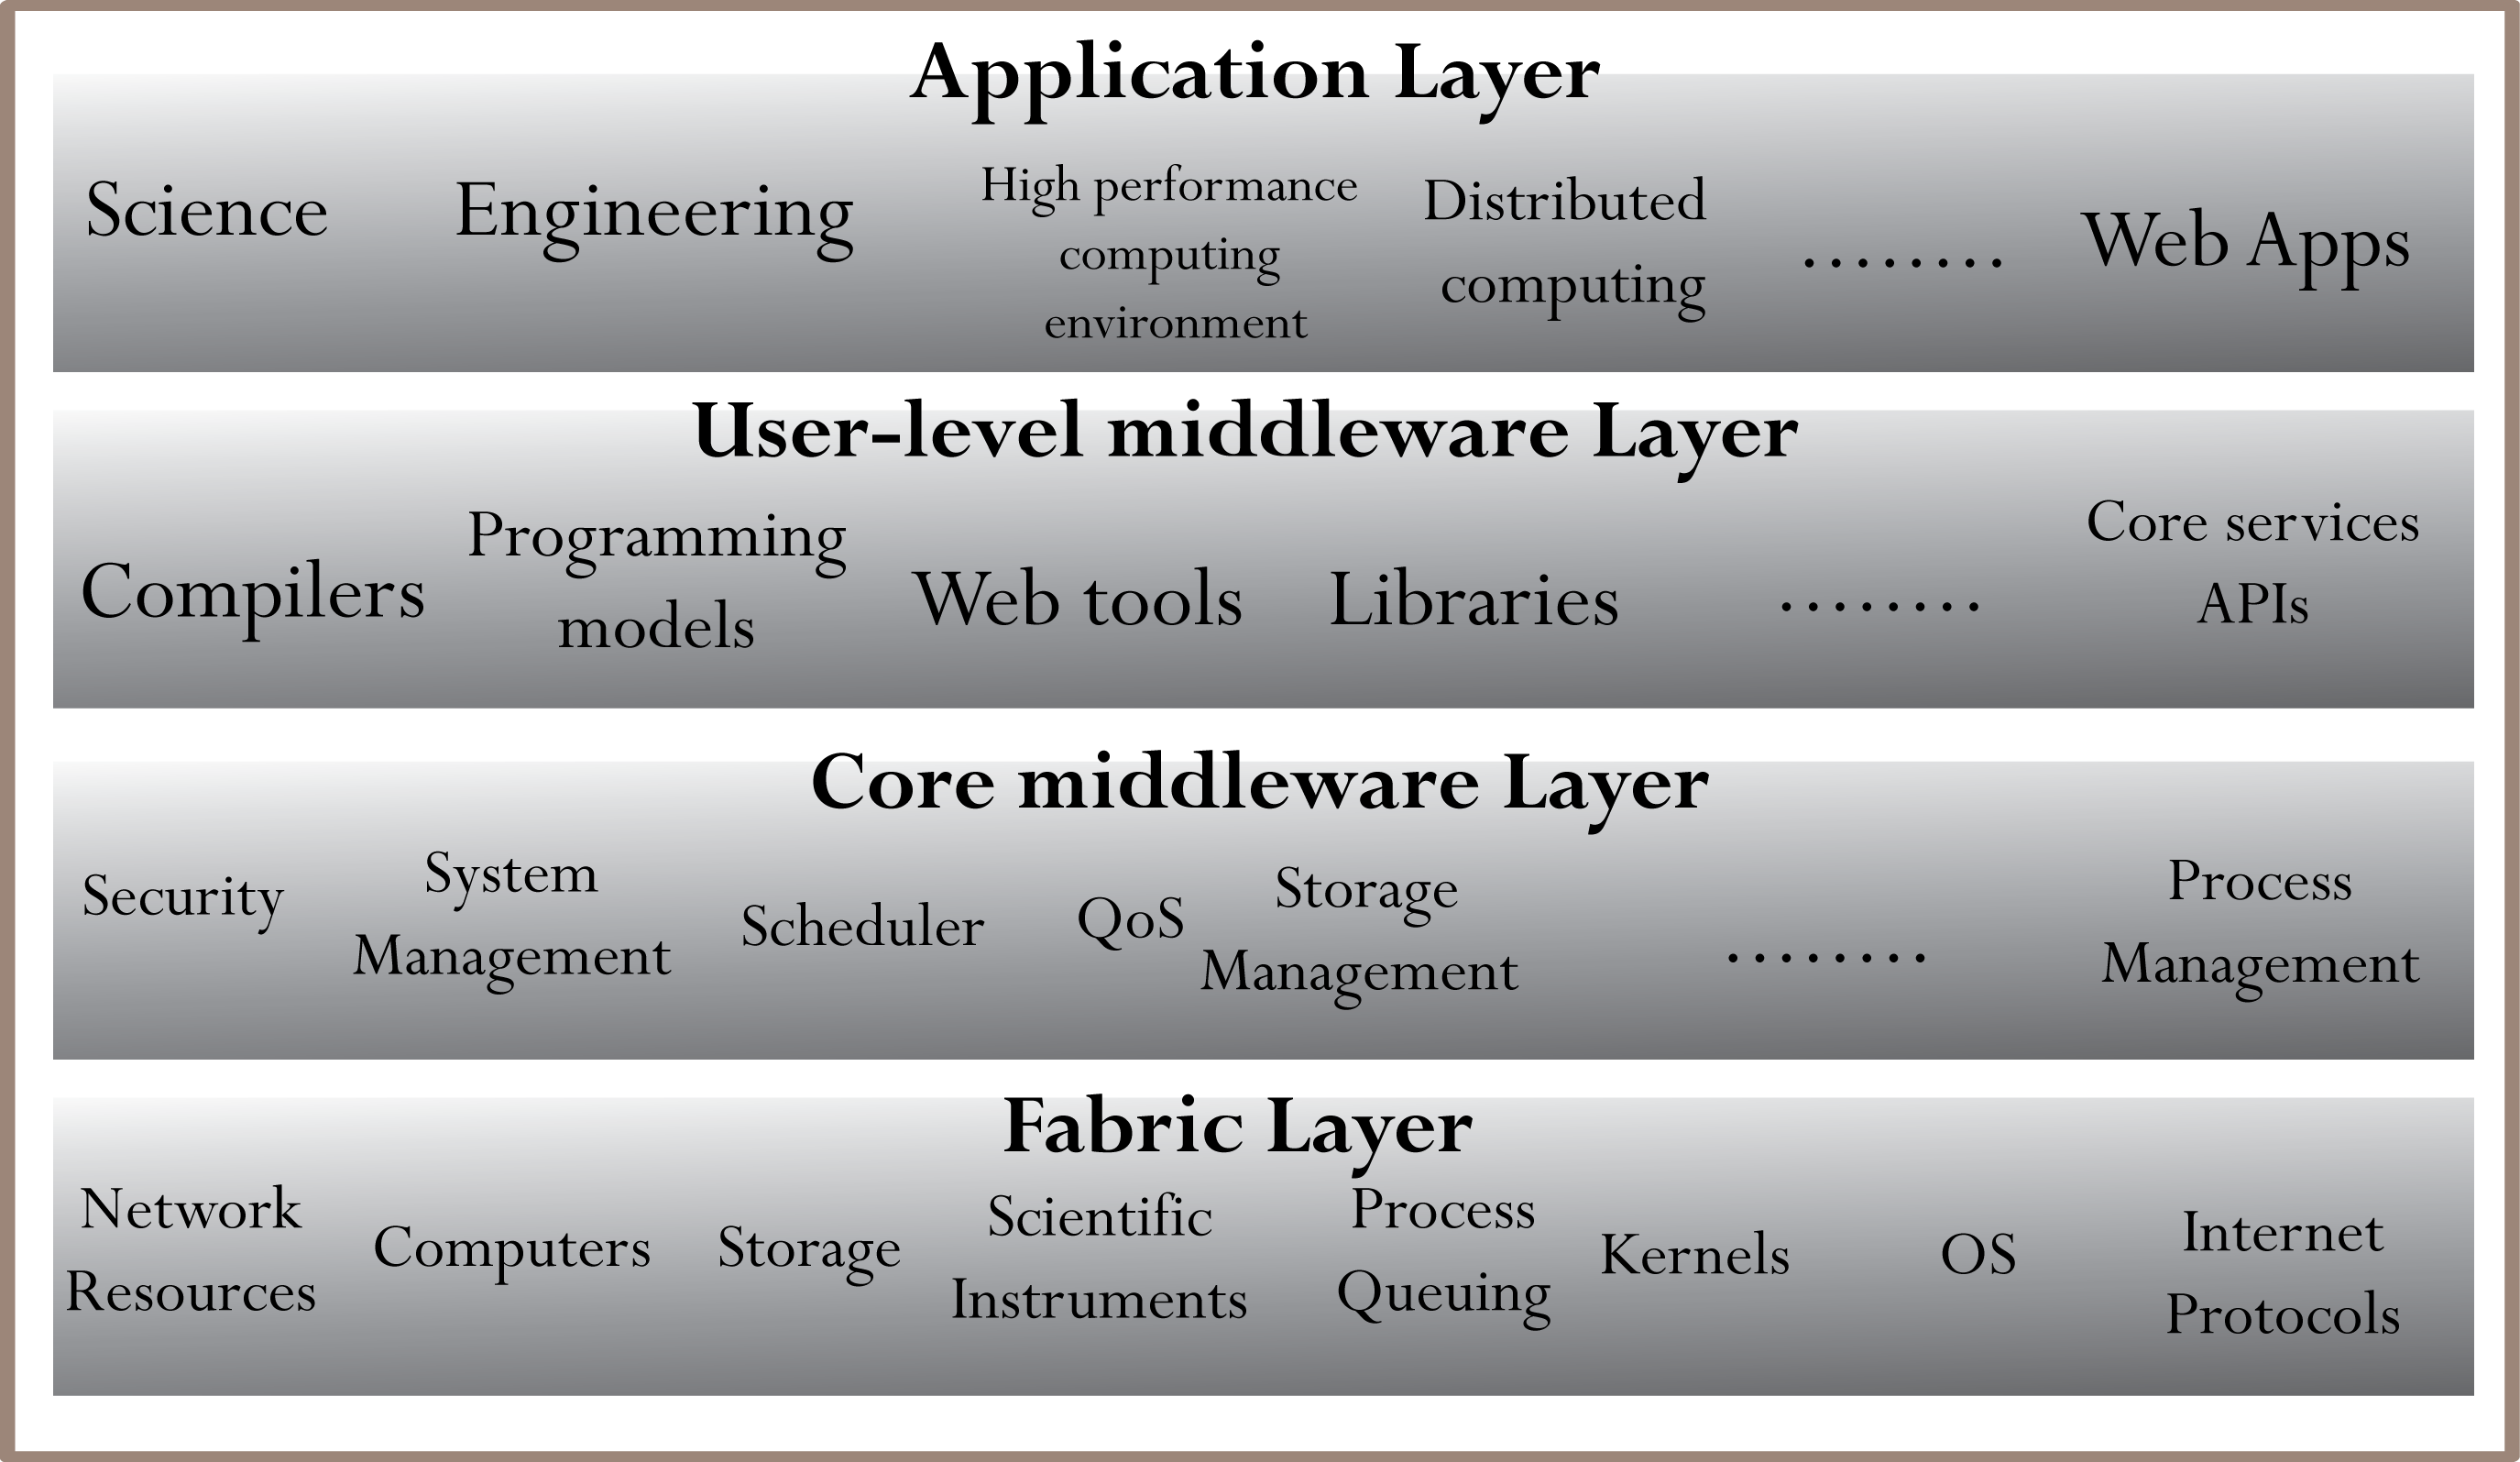
\includegraphics[width=1.0\columnwidth]{architecture}
    \caption{Grid Architecture and components}
	\label{fig:arch}
\end{figure}
\section{Grid Architecture}
Grid architecture \cite{buyya2005gentle} is described in layers, where each layer has some set of functions. Upper layers are application and user centric and lower layers are hardware centric. It consists of four layers i.e., application and portal layer, user-level middleware layer, core middleware layer and fabric layer. Figure~\ref{fig:arch} shows the stack within a grid architecture.
\begin{itemize}
 \item \textbf{Fabric layer:} The lower layer of grid architecture consists of network components, distributed resources, storage devices etc. Computational resources represent multiple architectures such as clusters, supercomputers, servers, ordinary PCs and even PDAs.
 \item \textbf{Core Middleware layer:} The middleware layer is referred to as the ``brains`` behind a computing grid. It provides tools for managing grid elements. It offers services like remote process management, allocation of resources, storage access, resource information registration/discovery, security, and Quality of Service (QoS).
 \item \textbf{User-level Middleware:} This layer helps users to build applications for grid with application development environment and various sets of programming tools. It has access to API's provided by the core middleware layer. 
\item \textbf{Application layer:} This is the layer users interact with. This includes applications in engineering, science, business, finance and more. This also provide development toolkits to support the applications. Grid portals can also offer scalable web-based application services. 
\end{itemize}

\section{Grid job scheduler}
Grid performance can be improved in terms of job processing time by making sure that all the resources available in the grid are utilized optimally using a good job
scheduling algorithm. Job scheduler exists in many conventional distributed environment systems but in grid there are several characteristics that make the scheduling different and more challenging. Some of these characteristics are dynamic structure of the computational grid, high heterogeneity of resources, jobs and interconnection networks, existence of local policies on resources and local schedulers, the large scale of the grid system and security \cite{xhafa2010computational}.\\
The grid scheduler has to follow a series of steps \cite{nabrzyski2004grid} : (1) Collecting information of jobs submitted to the grid, (2) Collecting available resource information, (3) Computation of the mapping of jobs to selected resources, (4) Jobs allocation according to the mapping, and (5) Monitoring of job completion.
There are two types of scheduling :
\begin{itemize}
\item \textbf{Static scheduling:} Jobs are statically assigned to resources before their execution begins. The jobs can not be rescheduled or interrupted once its execution starts.
\item \textbf{Dynamic scheduling:} Re-evaluation is allowed of already taken assignment decisions during job execution is allowed\cite{chtepen2005dynamic} . It can trigger job migration or interruption, based on dynamic information about the status of the system and the workload.
\end{itemize}
The Job scheduling in Grid can be correlated with a classical problem, Flexible Job-shop Scheduling problem(FJSP) \cite{brucker1990job} with dynamic changes of resources and their availability. Besides these grid jobs need to be scheduled as soon as possible after they are enqueued in the job queue, granting the scheduler only a few minutes of time to find the scheduling strategy. FJSP consists of routing subproblem and the scheduling subproblem \cite{wang2012enhanced}. Routing problem is to assign each job with a resource among a set of resources and scheduling problem is to obtain a feasible and satisfactory sequence of jobs within the resources.\\
Computationally, FJSP is as hard as JSP which is an NP Hard problem\cite{garey1979computers} . So finding near optimal solution in polynomial time is our aim. The problem becomes even more interesting when multiple objectives are there to be taken care of.  Nearly all job scheduling algorithms work on single objective like makespan (classical FJSP minimize makespan only).\\
Finding near optimal solution for FJSP problem with more than one objective in a time efficient way is a difficult task. Grid environment being dynamic in nature, reallocation of jobs is quite evident in it. \\
Our approach of solving the above problem using Non-dominated sorting evolutionary algorithm for minimization of multiple objectives, is well enough to find near optimal scheduling strategy in time. The running time complexity of algorithm is $O(GMN^2)$ where $G$ is the number of generations or iterations, $M$ is the number of objectives and $N$ is the population size of the chromosomes or scheduling strategies to run the algorithm.\\

\section{Motivation}
Grid aims at aggregating widely distributed resources and providing low cost computing resources to users. Resources can be computers, storage space, network resources connected through internet or private network with a middleware providing management capability. An Essential part of a Grid system is an efficient scheduling system i.e. resource sharing problem in dynamic and multi-institutional organizations \cite{foster2001anatomy}. Grid scheduling algorithms are inspected with different perspectives, such as static vs. dynamic, application models, QoS constraints, objective functions. Maximum utilization of grid resources is the most cogitated objective in scheduling literatures. However other factors like maintaining QoS constraints, cost effectiveness, energy efficient scheduling were either discussed separately or not acknowledged. Fair amount of importance should be given to user satisfaction, time and cost deadline of jobs. In 2007, Gartner estimated that the Information and Communication Technology industry is liable for 2\% of the global $CO_2$ emission annually, which is equal to that from the aviation industry \cite{pettey2007gartner}. A study done at the Lawrence Berkeley National Laboratory shows that the cooling efficiency (the ratio of computing power to the cooling power) of data centers varies drastically from a low value of 0.6 to a high value of 3.5 \cite{greenberg2006best}. \\
Above mentioned facets clearly show an urgency for a multi-objective grid scheduler, dealing them on their gravity of importance.
\section{Contribution of this thesis}
We present a multi-objective Job scheduler based on an evolutionary algorithm. The aim of this work is to give grid administrators a better scheduler, which will give better grip on the trade off among cost, utilization, energy efficiency and QoS. The scheduler can cope up with the dynamic behavior of resources, resource constraints and predecessor job constraints. A job grouping mechanism is proffered for fine grained jobs. \\
Pareto front approach is taken in multi-objective optimization. Non-dominating sorting mechanism with avant-garde crossover and mutation operator enables the scheduler to explore the search space minutely.\\
Objective functions can be classified into two categories: application-centric and resource-centric. Negotiation and trade off between two types of objectives is necessary. Our generalized multi-objective scheduler provides options to add and remove objective functions.
\section{Organization of the Thesis}
The organization of the rest of the thesis and a brief outline of the chapters
is as follows.
In chapter 2, some related works on job scheduling in grids and their merits and demerits have been discussed.
In chapter 3, Multi-objective Evolution based Dynamic Job Scheduler in Grid has been presented. Here problem definition, job-grouping strategy, problem formulation, MOJS module and algorithms are described.
In Chapter 4, implementation details and experimental results are given.
Chapter 5 sums up the work with conclusion and future work.
	\chapter{Related Work}
Job shop scheduling problem is at least 70 years old. Considerable effort to solve it and find computational complexity has been found to be in 1960 \cite{manne1960job}. This has been proven to be an NP-complete problem in 1979 \cite{jis1979computers}. Many researcher have used heuristic based solving approach to address the problem. Local Search \cite{ritchie2003fast}, Tabu search \cite{abraham2000nature}, simulated Annealing \cite{yarkhan2002experiments} \cite{abraham2000nature} are single heuristic based approach. \\
In Tabu search, one solution $s$ moves to another solution $s'$ located in the neighborhood with a slight modification possible from $s$. Tabu search overcomes the local optimality with a steepest descent/mildest ascent approach. However performance of TS largely depends on the parameters and heuristic used in formulating the problem. For multi-objective scheduling TS might not be sufficient. 

In simulated annealing technique, each solution is mutated and if the mutant spawned exceeds threshold it is rejected, and if less than or equal to the energy of the parent, the difference of threshold and energy of mutant is added to Energy Bank(EB). The  threshold is changed when EB reaches a certain value and population moved to new generation. Simulated annealing mutation/reheating is directly proportional to the energy accumulated in EB. Simulated annealing in Multiobjective domain e.g. AMOSA \cite{bandyopadhyay2008simulated} requires many parameters and domination factor to find near optimal solutions, which are hard to established in grid scheduling.

There are also some hybrid approaches like Tabu search with Ant colony Optimization \cite{ritchie2003static} \cite{ritchie2004hybrid}, GA's with Simulated annealing \cite{zheng2006task}.Other predictive model approaches for the problem are Particle Swarm optimization \cite{liu2010scheduling}  \cite{abraham2006scheduling}, Fuzzy based scheduling \cite{kumar2004fuzzy}. AI based scheduling algorithms like Max-min (Task with more computation time has higher priority), Min-min (Task with less computation time has higher priority), Suffrage (Task with higher sufferage value is given higher priority, its value is determined as the difference of computational time between best and second best resources on which job can be allocated)\cite{ibarra1977heuristic}. All the above work have focused on single objective i.e. minimizing the makespan, which in turn maximizes the utilization of resources. Resource constraint was also not taken into consideration.

Job grouping based scheduling algorithm is used for fine-grained jobs \& light-weight jobs which increase the resource utilization \cite{muthuvelu2005dynamic}  \cite{ang2009bandwidth} . The later have considered communication and bandwidth capabilities. However they have not taken care of predecessor job completion constraint and dynamic behavior of resources in grid.

Genetic algorithms are a stochastic search method introduced in the 1970s in the United States by John Holland [Holland 76] and in Germany by Ingo Rechenberg [Rechenberg 73]. It is based on Darwin's natural selection principle of evolution of biological species. GA operate on a population of solution and apply heuristics such as selection, crossover, and mutation to find better solutions \cite{wall1996genetic}. 

EDSA is a GA’s searching technique in which the crossover and mutation rates are changed dynamically depending on the variances of the fitness values in each generation \cite{yu2008evolution} . The scheduling consider minimization of makespan. 
MOEA  has addressed the need for multi-objective minimization on computational grid, their work was limited to one type of resource, two objectives i.e. makespan \& flowtime, and lacks predecessor job constraint \cite{grosan2007multiobjective}.

In our work based on multi-objective evolutionary algorithm we have converted resource scheduling problem in grid into \emph{resource-constrained project scheduling problem}. We have incorporated dynamic scheduling mechanism, advanced crossover and mutation operator \& minimizing five objectives with pareto front technique. The GA structure of Non-dominating Sorting Genetic Algorithm II proposed by K.Deb \emph{et al.} have helped us in creating the MOJS module \cite{deb2002fast}.

GA based scheduler can act as a real time scheduler due to increase in computational capability of processors in last five years.  We have proposed a job grouping strategy for fine-grained jobs, so that it can deliver job schedule to dispatcher on time. \\
A comparable work with matching constraints could not be found in literature, only few publications deal with multi-objective scheduling \cite{grosan2007multiobjective} but their platform is different from ours. So in result section we experimented our scheduler and produced result on the performance based on various parameters.\\

        \chapter{Multi-objective Evolution based Dynamic Job Scheduler in Grid}

\section{Problem Definition}
Grid is a distributed decentralized heterogeneous computational system, later it has also incorporated network storage system. User applications run on Grid varies from lightweight to extensive computational/storage application with various constraints. Job Scheduler is responsible to select best suitable machines in this grid for each job. In large grid this should be done automatically. The scheduling system generates job schedules for each machine in the grid by considering predefined static constraints of jobs and machines and dynamic behavior of grid. Grid environment is highly dynamic, resources can join and leave grid any time.\\
We define the problem in three sections as follows: 
\subsection{Flexible Job Shop Scheduling}
The typical job-shop problem is formulated as a work order that consists of set of $n$ jobs, each of which contains $m$ tasks. Each task has predecessors and requires a certain type of resource, i.e. to be processed by any machine from a given set \cite{wall1996genetic}. Often many resources of a specific type are available, for example five milling machines and two lathes. Many tasks can be assigned to any one of the available resources, but the resource must be of the suitable type. Similarly in the computing environment some computational jobs have certain requirement specifications and resource types to maintain their quality of service. Typical objectives for scheduling include minimizing the makespan for the work order. Here we are also considering energy consumption, time limit constraint, cost constraint and maximize utilization of resources as objectives.
\subsection{Dynamic Scheduler}
Dynamic scheduler considers dynamic environment of grid where resources can change its configuration and availability. In dynamic scheduling re-evaluation is allowed for already taken assignment decisions during job execution \cite{chtepen}. It can trigger job migration or interruption based on dynamic information about the status of the system and the workload. When a resource leaves grid system the Grid Information Service (GIS) can trigger the scheduler to reschedule the queued jobs among the available resources. However care should be taken on scheduling the jobs that are dependent on the rescheduled jobs. Similarly addition of new resources will trigger reshuffling of the jobs for proper utilization of resources though less complexities are involved in this case. Section ~\ref{dynamicscheduling} addresses this problem.
\subsection{Gridlet}
Grid job is often referred to as Gridlet. Jobs can be fine as well as coarse grained. In grid computing, MI is the unit of job size. MI is million instructions or processing requirements of a user job \cite{liao2009research}. If the MI of a job is less than a fixed threshold $M$, it is a fine-grained job. Similar approach i.e. Megabytes(MB) parameter is used for storage intensive jobs. For fine-grained jobs, a job-grouping strategy is suggested for faster execution of scheduler in section ~\ref{jobgr}.
\begin{figure}[ht]
    \centering
    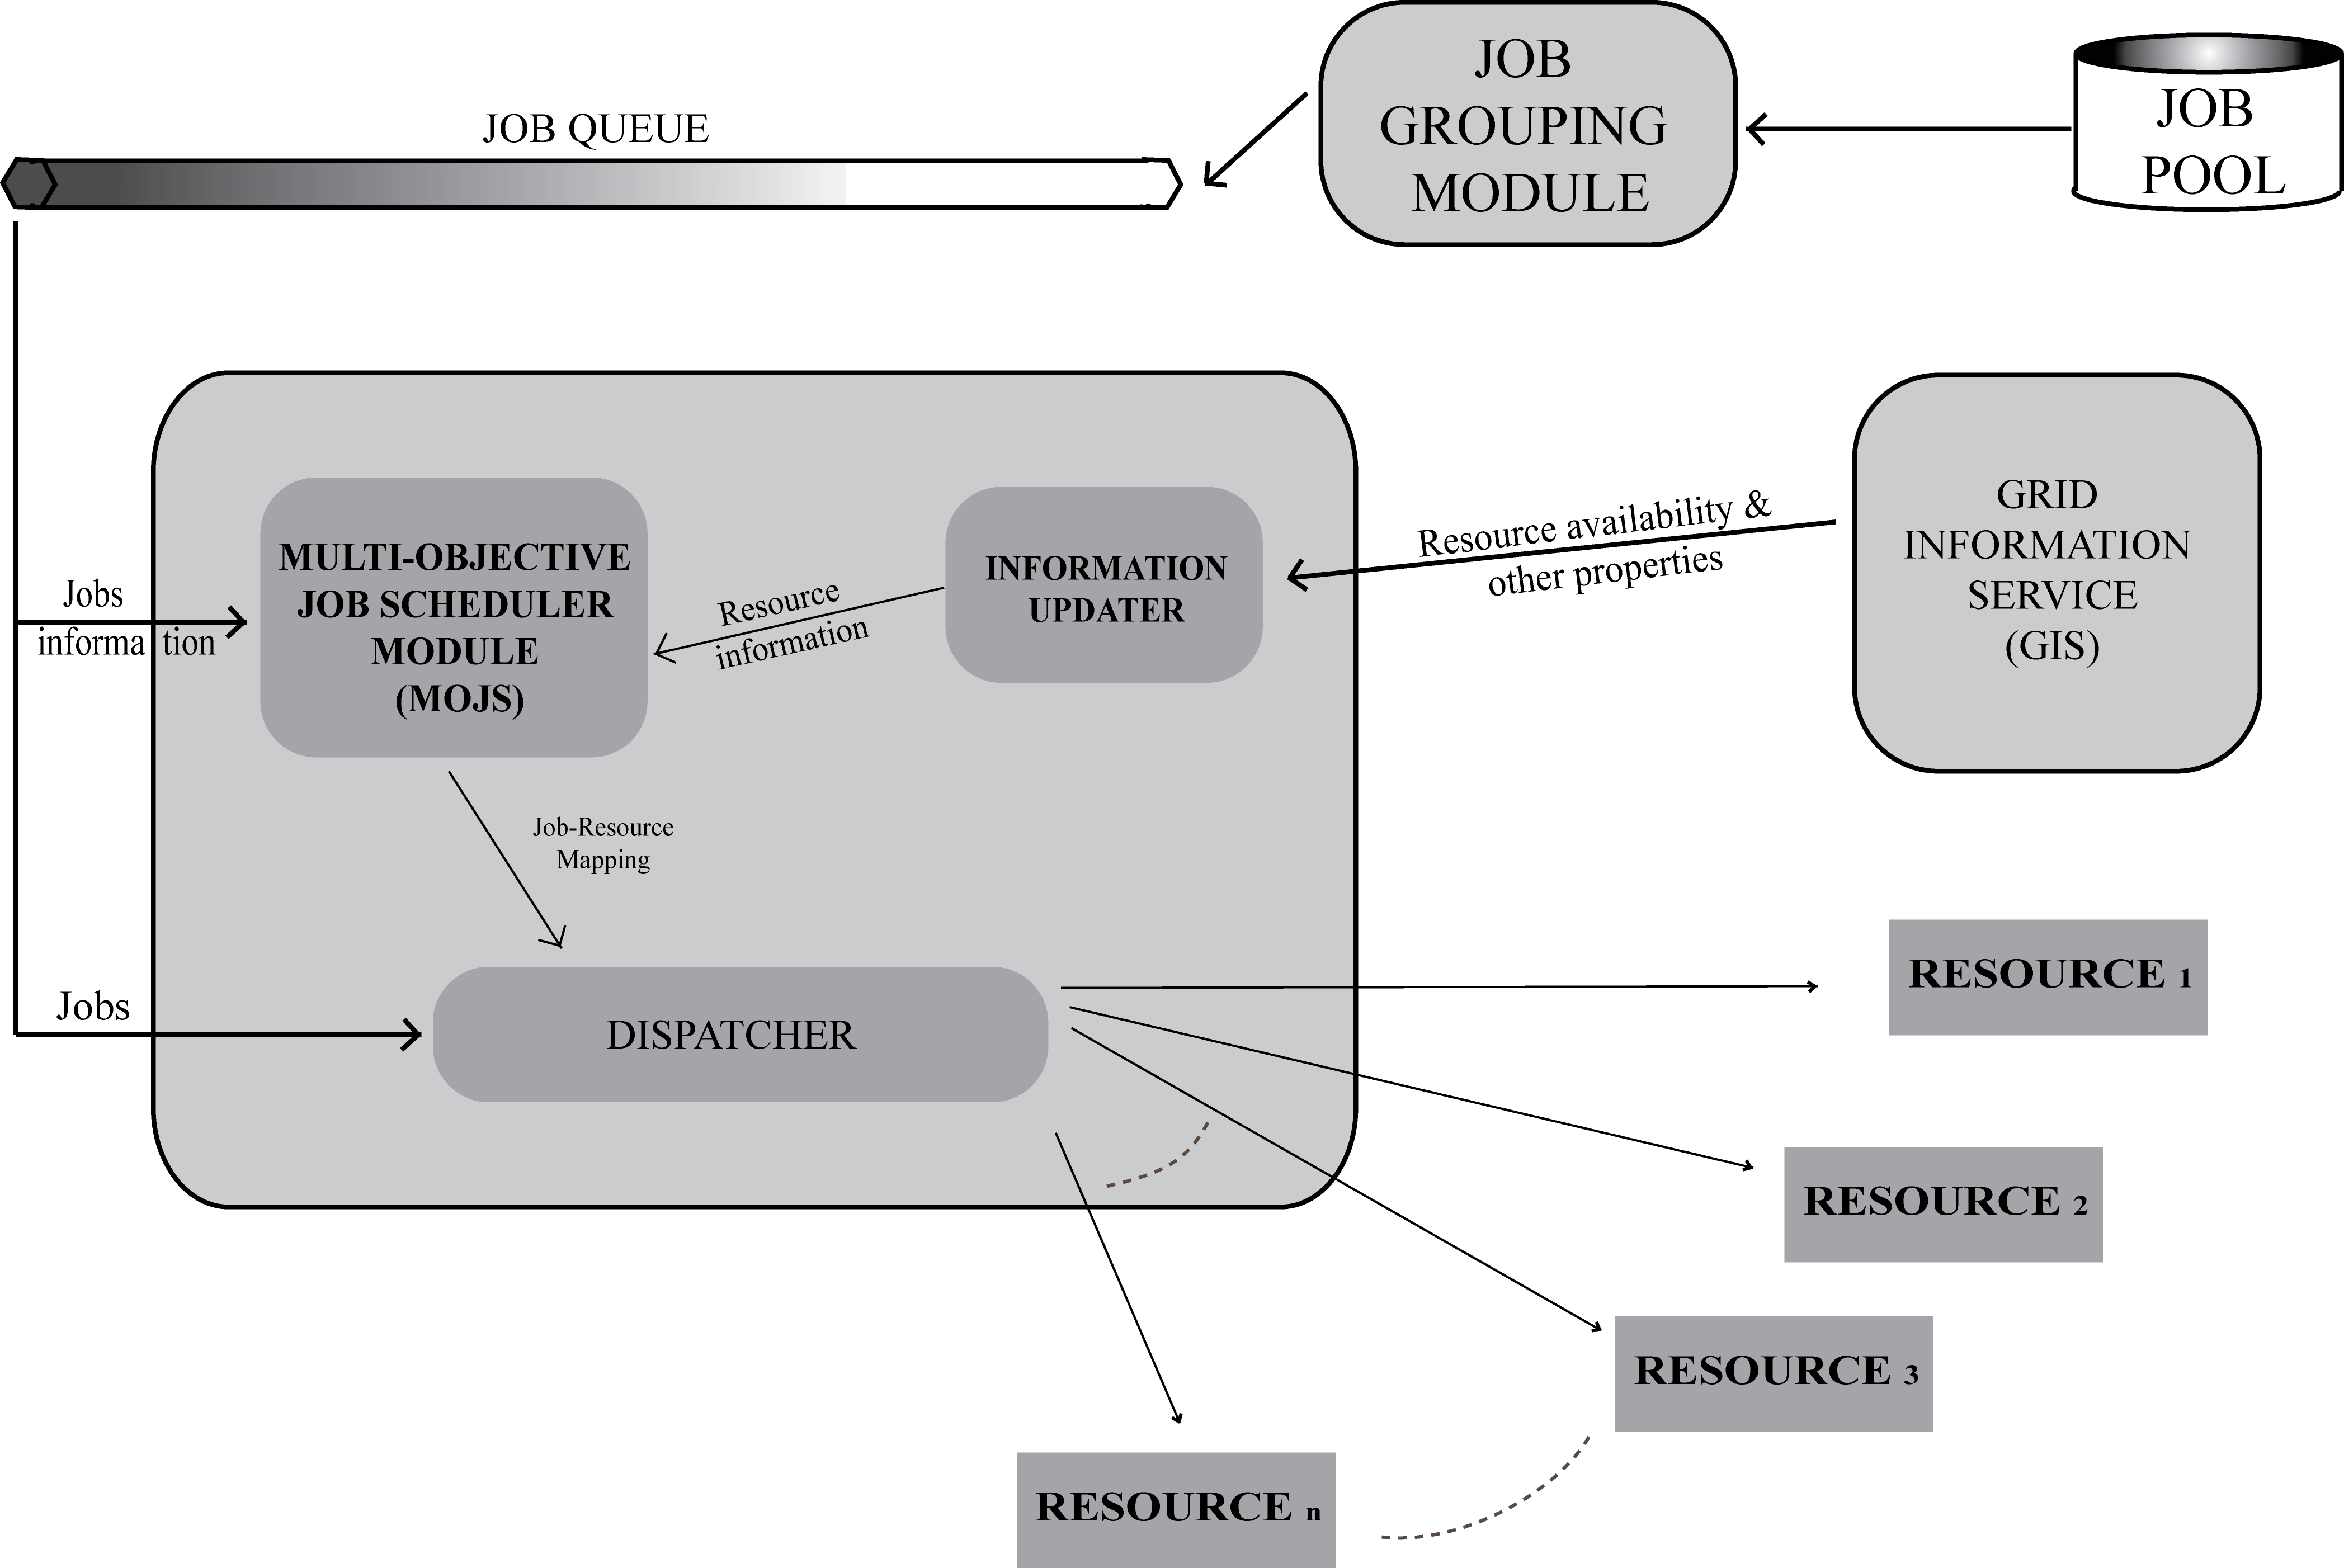
\includegraphics[width=1.0\columnwidth]{scheduler}
    \caption{Scheduling Model}
	\label{fig:Scheduling Model}
\end{figure}

\section{Job Scheduling Model}
The four basic building blocks of grid model are as follows 
\begin{itemize} 
 \item Users 
 \item Job scheduler 
 \item Grid Information System (GIS) 
 \item Resources
\end{itemize}
 The user submits a list of jobs to the job pool where it gets a unique identification number i.e. Job ID. If necessary job-grouping of very fine-grained jobs is accomplished by meta-scheduler before the scheduler process these jobs. The scheduler obtains information of resources from Grid Information Service (GIS). GIS provides information like resource availability, processing capability, energy consumption and cost details. Based on the information, a scheduling strategy i.e. mapping of jobs with execution start time and resources is created and send to dispatcher. The dispatcher dispatch jobs to their corresponding resources on time and collects the results of completed jobs from the resources.

\section{Formulation of problem}
\label{formulation}
Here the problem is formulated with the notations described in scheduling literature \cite{brucker2004scheduling}, \cite{brucker2006scheduling}, \cite{jakob2008fast}. Given are a set $M = \{M_1, M_2, M_3, ... M_m\}$ of resources, a set $J = \{J_1, J_2, J_3, ... J_j\}$ of application jobs, and a set $O$ of grid jobs. The n Grid Jobs of application job $J_i$ are denoted by $O_{i1},..., O_{in}$, a set $W= \{W_1,W_2,\ldots,W_m\}$ denotes normalized energy dissipation factor of resources. Table ~\ref{notation1} gives a concise definition of the notations have been used.\\
\begin{table}[!ht]
\caption{Notation Symbol and their definitions}
\centering
    \begin{tabular}{|c|l|}
    \hline \hline
    Notation & Definition  \\ \hline
    $M_i$ & Resource with ID $i$ \\ \hline
    $J_i$ & Application job with ID $i$ \\ \hline
    $O_{ij}$ & $j$th Grid Job or task of Application job $J_i$ \\ \hline
    $W_i$ & Energy dissipation factor of Resource $M_i$, \\
	  & normalized with the max value from set $W$ \\ \hline
    $t(O_{ij},R_{ij})$ & Processing time of $O_{ij}$ mapped to resource $R_{ij}$ \\ \hline
    $c(O_{ij},R_{ij})$ & Cost of $O_{ij}$ mapped to resource $R_{ij}$ \\ \hline
    $s(O_{ij})$ & Start time of job $O_{ij}$ \\ \hline
    $e(O_{ij})$ & End time of job $O_{ij}$ \\ \hline
    $d_{ij}$ & Time limit for completion of $O_{ij}$ \\ \hline
    $c'_{ij}$ & cost limit for  $O_{ij}$ \\ \hline
    $tsum(M_i)$ & Running time or Uptime of $M_i$ \\ \hline
    \end{tabular}
\label{notation1}
\end{table}
\textbf{The following functions are used:}
\begin{itemize}
  \item A precedence function 
  \subitem $p:O$x$O \rightarrow \{ TRUE,FALSE\}$ for the grid jobs.
  \item An assignment function $\mu:O \rightarrow P(P(M))$ from grid jobs to resource sets. $P(M)$ is the power set of $M$. $\mu_{ij}$ is the set  of all possible combinations of resources from $M$, which together are able to perform the grid job $O_{ij}$
  \item Resource mapping $R: O \rightarrow P(P(M)) $, $R_{ij}$ represent mapping of job $O_{ij}$ on a machine $M$, $R_{ij} \in \mu_{ij}$
  \item Function $t:O$x$P(M) \rightarrow \mathbb{R}$, which gives for every grid job $O_{ij}$ the time needed for processing on a resource set $R_{ij} \in \mu_{ij}$
  \item Cost function $c: O$x$P(M) \rightarrow \mathbb{R}$, $c(O_{ij},R_{ij})$ is the cost of job $O_{ij}$ mapped on resource $R_{ij}$.
  \item Function $l:M_i  \rightarrow O_{jk}$ which gives the last grid job executed on resource $M_i$
  \item Function $s:O_{ij} \rightarrow \mathbb{R}$, $s(O_{ij})$ is the start time of grid job $O_{ij}$.
  \item Function $e:O_{ij} \rightarrow \mathbb{R}$, $e(O_{ij}) = s(O_{ij}) + t(O_{ij},R_{ij})$ is the end time of grid job $O_{ij}$ which is mapped on resource $R_{ij}$.
  \item Function $tsum : M_i \rightarrow \mathbb{R}$ which gives the resource $M_i$ running time or Uptime.
\end{itemize}
Optimization is done by choosing suitable start times $s(O_{ij}) \in \mathbb{R}$ and resource allocations $R_{ij} \in \mu_{ij}$. A solution is valid, if the following two \textbf{restrictions} are met:
\begin{enumerate}
  \item All grid jobs are planned and resources are allocated exclusively:
  \subitem $ \forall O_{ij} : \exists s(O_{ij}) \in \mathbb{R}, R_{ij} \in \mu_{ij} : \forall M_j \in R_{ij} $:
  \subitem $M_j$ is in $[s(O_{ij});s(O{ij})+t(O_{ij}),R_{ij}]$ exclusively allocated by $O_{ij}$
  \item Precedence relations are adhered to: 
  \subitem $\forall i, j \neq k : p(O_{ij},O_{ik}) \Rightarrow s(O_{ik}) \geq s(O_{ij}) +t(O_{ij}, R_{ij})$
\end{enumerate}
Exceeding the time limit and budget cost will affect QoS of grid jobs. A penalty factor is imposed when jobs violates following \textbf{constraints}.
\begin{enumerate}
  \item All grid jobs $O_{ij}$ have time limit $d_{ij}$ which must be adhered to:
  \subitem $ \forall O_{ij} : d_{ij} \geq s(O_{ij}) + t(O_{ij},R_{ij}) $:
  \item All grid jobs $O_{ij}$ have a cost limit  $c'_{ij}$ which must be adhered to: 
  \subitem $\forall O_{ij} : c'_{ij} \geq c(O_{ij},R_{ij}) $
  
\end{enumerate}
\textbf{This work focuses on achieving near-optimal scheduling strategy on following objective functions}:
\begin{enumerate}
  \item Minimizing makespan, $e(O_{ij})$ is the end time of grid job $O_{ij}$
  \subitem $ f_1 =makespan = max\{e(l(M_1)),e(l(M_2)),\ldots,e(l(M_m)) \}$
\begin{framed}
Makespan is the time at which all the resources becomes free.
\end{framed}
  \item Maximizing utilization of resources i.e. minimizing $f_2$
  \subitem $ f_2 = non-utilization = \frac{1}{m} \sum_{j=1}^{m}  \{e(l(M_j)) - tsum (M_j)\}$
\begin{framed}
$f_2$ is the average time period during which the the resources are idle.
\end{framed}
  \item Minimizing time limit penalty (minimizing number of jobs completing after due date)

$$
f_3 = \frac{1}{j*n}  \sum_{\forall i,j} \varphi _1 (e(O_{ij}) - d_{ij}) 
$$
where $\varphi _1(x)$ is a non-negative continuous exponential non-decreasing function, if $x > 0$ else $0$.

\begin{framed}
The grid jobs failed to complete within time limit contribute to the \par penalty function $f_3$. Minimizing time limit penalty is our aim.
\end{framed}
  \item Minimizing cost penalty 
$$
f_4 = \frac{1}{j*n}  \sum_{\forall i,j} \varphi _2 \{c(O_{ij},R_{ij}) - c'_{ij}\} 
$$
where $\varphi _2(x)$ is a non-negative continuous linear non-decreasing function, if $x > 0$ else $0$.

\begin{framed}
The grid jobs failed to meet the cost limit constraint contribute to the \par penalty function $f_4$. Minimizing cost limit penalty is our aim.
\end{framed}
  \item Minimizing Overall Energy consumption
  \subitem $f_5 = \sum_{i=1}^{m} tsum(M_i) * W_i$
\begin{framed}
$f_5$ gives energy consumption of all the resources.
\end{framed}
\end{enumerate}

\section{MOJS Module}
On submission of jobs and grid resource infromation to Multi-Objective Job Scheduler (MOJS) module, it outputs a near optimal scheduling strategy. Some of the important building blocks of scheduler are discussed below.
\subsection{Multi-objective optimization}
Generalized multi-objective optimization problem can be described as:\\
Minimize $y = f(x) = (f_1(x),f_2(x),\ldots,f_k(x))$\\
where $x \in \mathbb{V}, y \in \mathbb{R}^k$\\
where, $x$ is decision vector in search space $\mathbb{V}$, $y$ is the objective vector with $k > 1$ objectives.
\subsection{Chromosome model}
A scheduling strategy or mapping of jobs on resources satisfying the constraints is represented by  chromosome. A chromosome stores parameters as follows 
\begin {itemize}
\item Resource id corresponding to each job
\item Start time of every job
\item End time of every job
\item Predecessor job ID of each job 
\item Five objective function values 
\item Rank of chromosome, Rank is defined in section ~\ref{nds} 
\item Crowding distance, defined in section ~\ref{cds} 
\end{itemize}
Start time for execution of jobs is calculated according to heuristic rules (i) Schedule grid job as early as its precedent job is completed (ii) Schedule grid jobs according to shortest due date.
\subsection{Non-Dominated Sorting}
\label{nds}
A chromosome $a$ is said to be dominated by chromosome $b$ iff $\forall i \in \{1,2,\ldots,k\}: f_i(a) \leq f_i(b)$ and $\exists i \in \{1,2,\ldots,k\}: f_i(a) < f_i(b)$.
A chromosome $a$ is said to be Non-dominated if there does not exist any chromosome $b\in \mathbb{V}$ search space that dominates $a$. A set of such non-dominated chromosome in objective space is called pareto optimal front. After removing the pareto optimal front, a second pareto optimal front can be obtained. We assign a rank to each of the chromosome according to their occurrence in the pareto front. Then the algorithm sorts the population according to their rank and crowding distance (discussed in section~\ref{cds}) for selecting population for next generation. After a certain number of generations any chromosome from the first pareto front satisfying the soft constraints  can be chosen as the near optimal solution, or a weighted sum of the objectives can be used for finding suitable solution.
\subsection{Diversity preservation}
It is desired that the evolutionary algorithm maintains a good spread of solutions in the population, so that sustainable diversity in the population remains and solutions are not restricted to local optimization.
\subsubsection{Crowding distance}
\label{cds}
Crowding distance ($dist_x$) of a particular chromosome $x$ in population measures the density of chromosomes surrounding it. \\
After non-dominated sorting is completed, each chromosome's crowding distance is calculated as the sum of normalized distance between its adjacent neighbors corresponding to each objective. Crowding distance for first and last individual is infinite.\\

$dist_x = \sum _{j=1}^{k}\frac{f_j(x_{left})-f_j(x_{right})}{f_j^{max} -f_j^{min}}$
where $f_j$ is $j$th objective function, and number of objectives is $k$.
\subsubsection{Crowded comparison operator}
Each chromosome in the population will have two attributes
\begin{enumerate}
\item non-domination rank $r_x$
\item crowding distance $dist_x$
\end{enumerate}
\begin{framed}
A partial order $\prec$ between chromosomes are defined as:\\
$ a \prec b $ if $r_a \prec r_b$\\
or $(r_a = r_b)$ and $(dist_a \succ dist_b)$
\end{framed}
This means that we prefer a chromosome from less crowded region in search space in same front.
\subsection{NSGA II}
Non-dominated Sorting Genetic Algorithm II \cite{deb2002fast} is used as a basic framework for our Job scheduler module. In NSGA II, initially a random parent population $P_0$ is created. Using the above relation partial order population is sorted. For the first generation binary tournament selection, recombination, and mutation operators are used to create an offspring population $Q_0$ of same size as $P_0$ say $N$.\\
Now we describe the $t$th generation. A combined population $R_t = P_t \cup Q_t$ is formed of size $2N$. Then $R_t$ is sorted according to non-domination. Now best non-dominated set i.e. first pareto front $F_1$ is chosen for new population. If size of $F_1$ is less than $N$ then solutions from $F_2$ are chosen next, followed by $F_3$ and so on. Now a new population $P_{t+1}$ of size N is chosen  after crowding distance sorting.  This population is now used for selection, crossover, mutation to generate new offspring population $Q_{t+1}$ of size $N$ , and $R_{t+1}$ is formed by union of $P_{t+1}$ and $Q_{t+1}$. A schematic explanation of procedure is given in Figure ~\ref{NSGA2}.
\begin{figure}[!h]
    \centering
    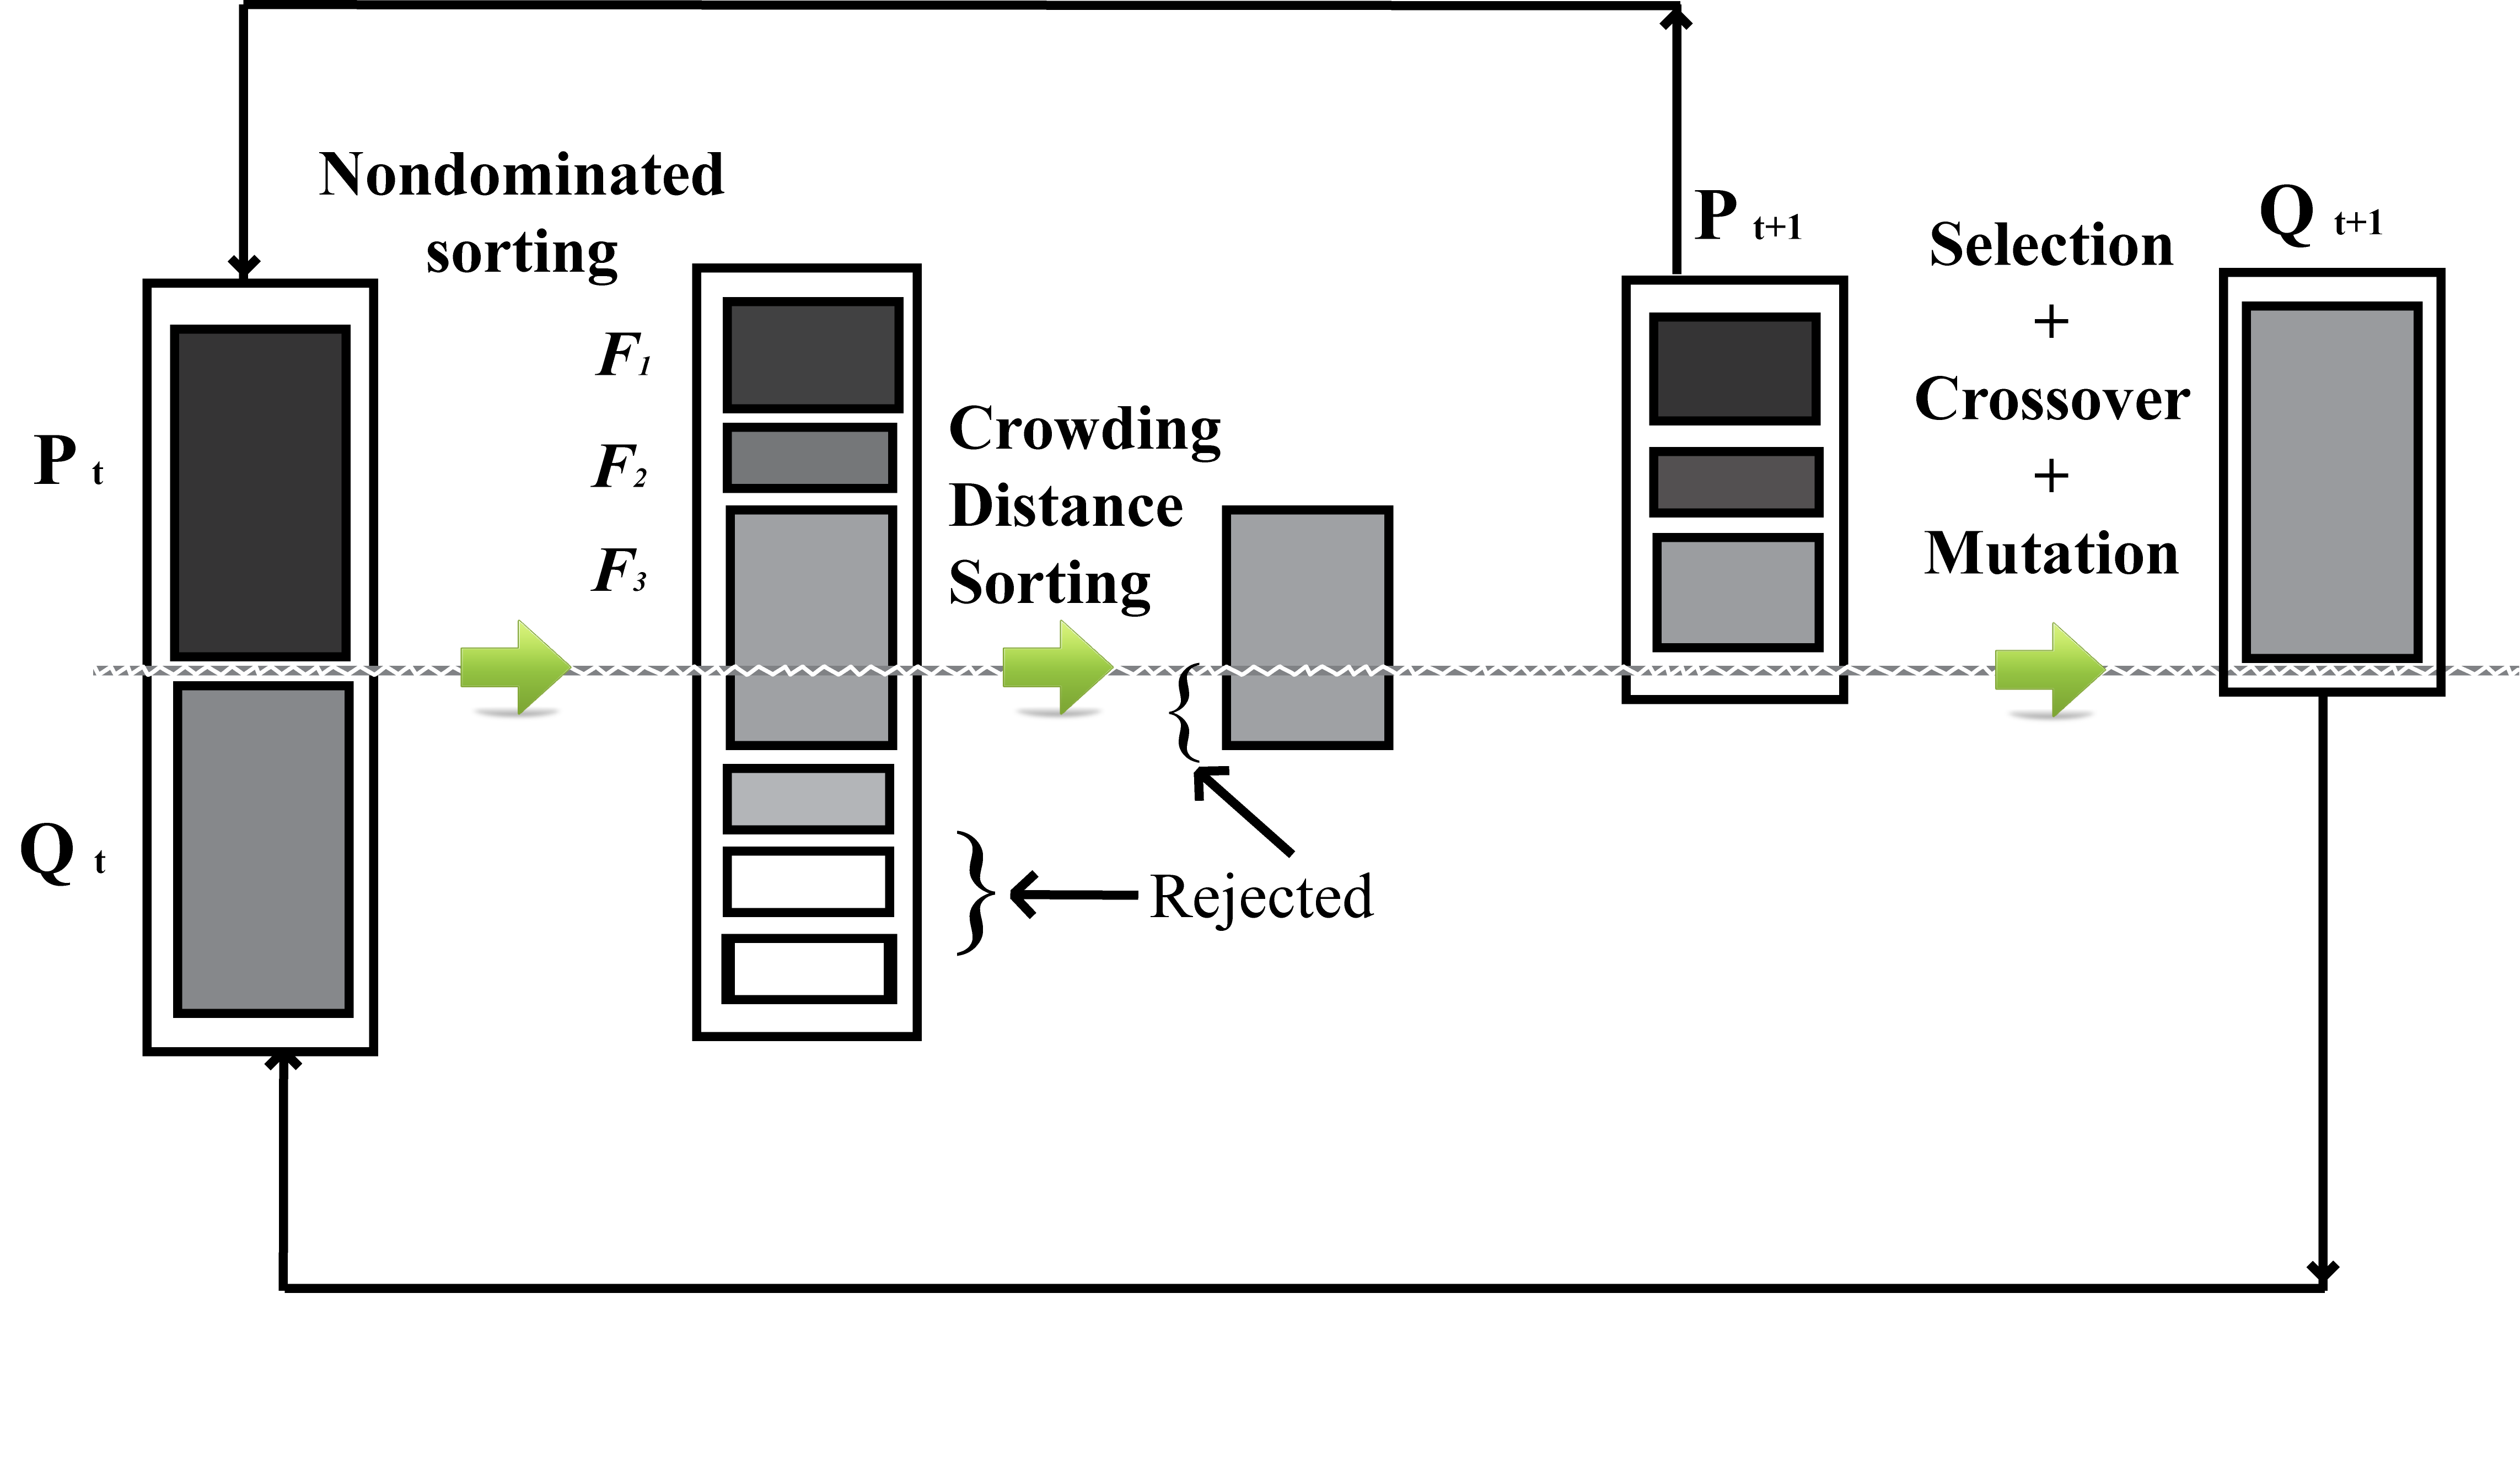
\includegraphics[width=1.0\columnwidth]{NSGA2}
    \caption{NSGA II procedure \cite{deb2002fast}}
	\label{NSGA2}
\end{figure}
\subsection{Crossover, Mutation and Elitism}
\subsubsection{Crossover}
The crossover operators are the most important part of any evolutionary-like algorithm. In each generation a mating pool of chromosomes is created through a tournament of selection among chromosomes. Two chromosomes are selected from mating pool interchanging their genes to obtain new individuals. The aim is to obtain new individual/chromosome with better fitness function and that will help in exploring new regions in search space not explored yet. $P_c$ is the probability with which crossover operator is applied.
Crossover operators depends on the chromosome representation.\\
\textbf{\emph{One point crossover: }} Given two parent chromosomes, this operator first randomly chooses a position between 1 and $NUM\_JOBS$. The point act as cutting point. Then the two first parts of the parents are interchanged yielding two new descendants. Schematic representation is given in Figure ~\ref{1pointxover}.\\
\begin{figure}[!h]
    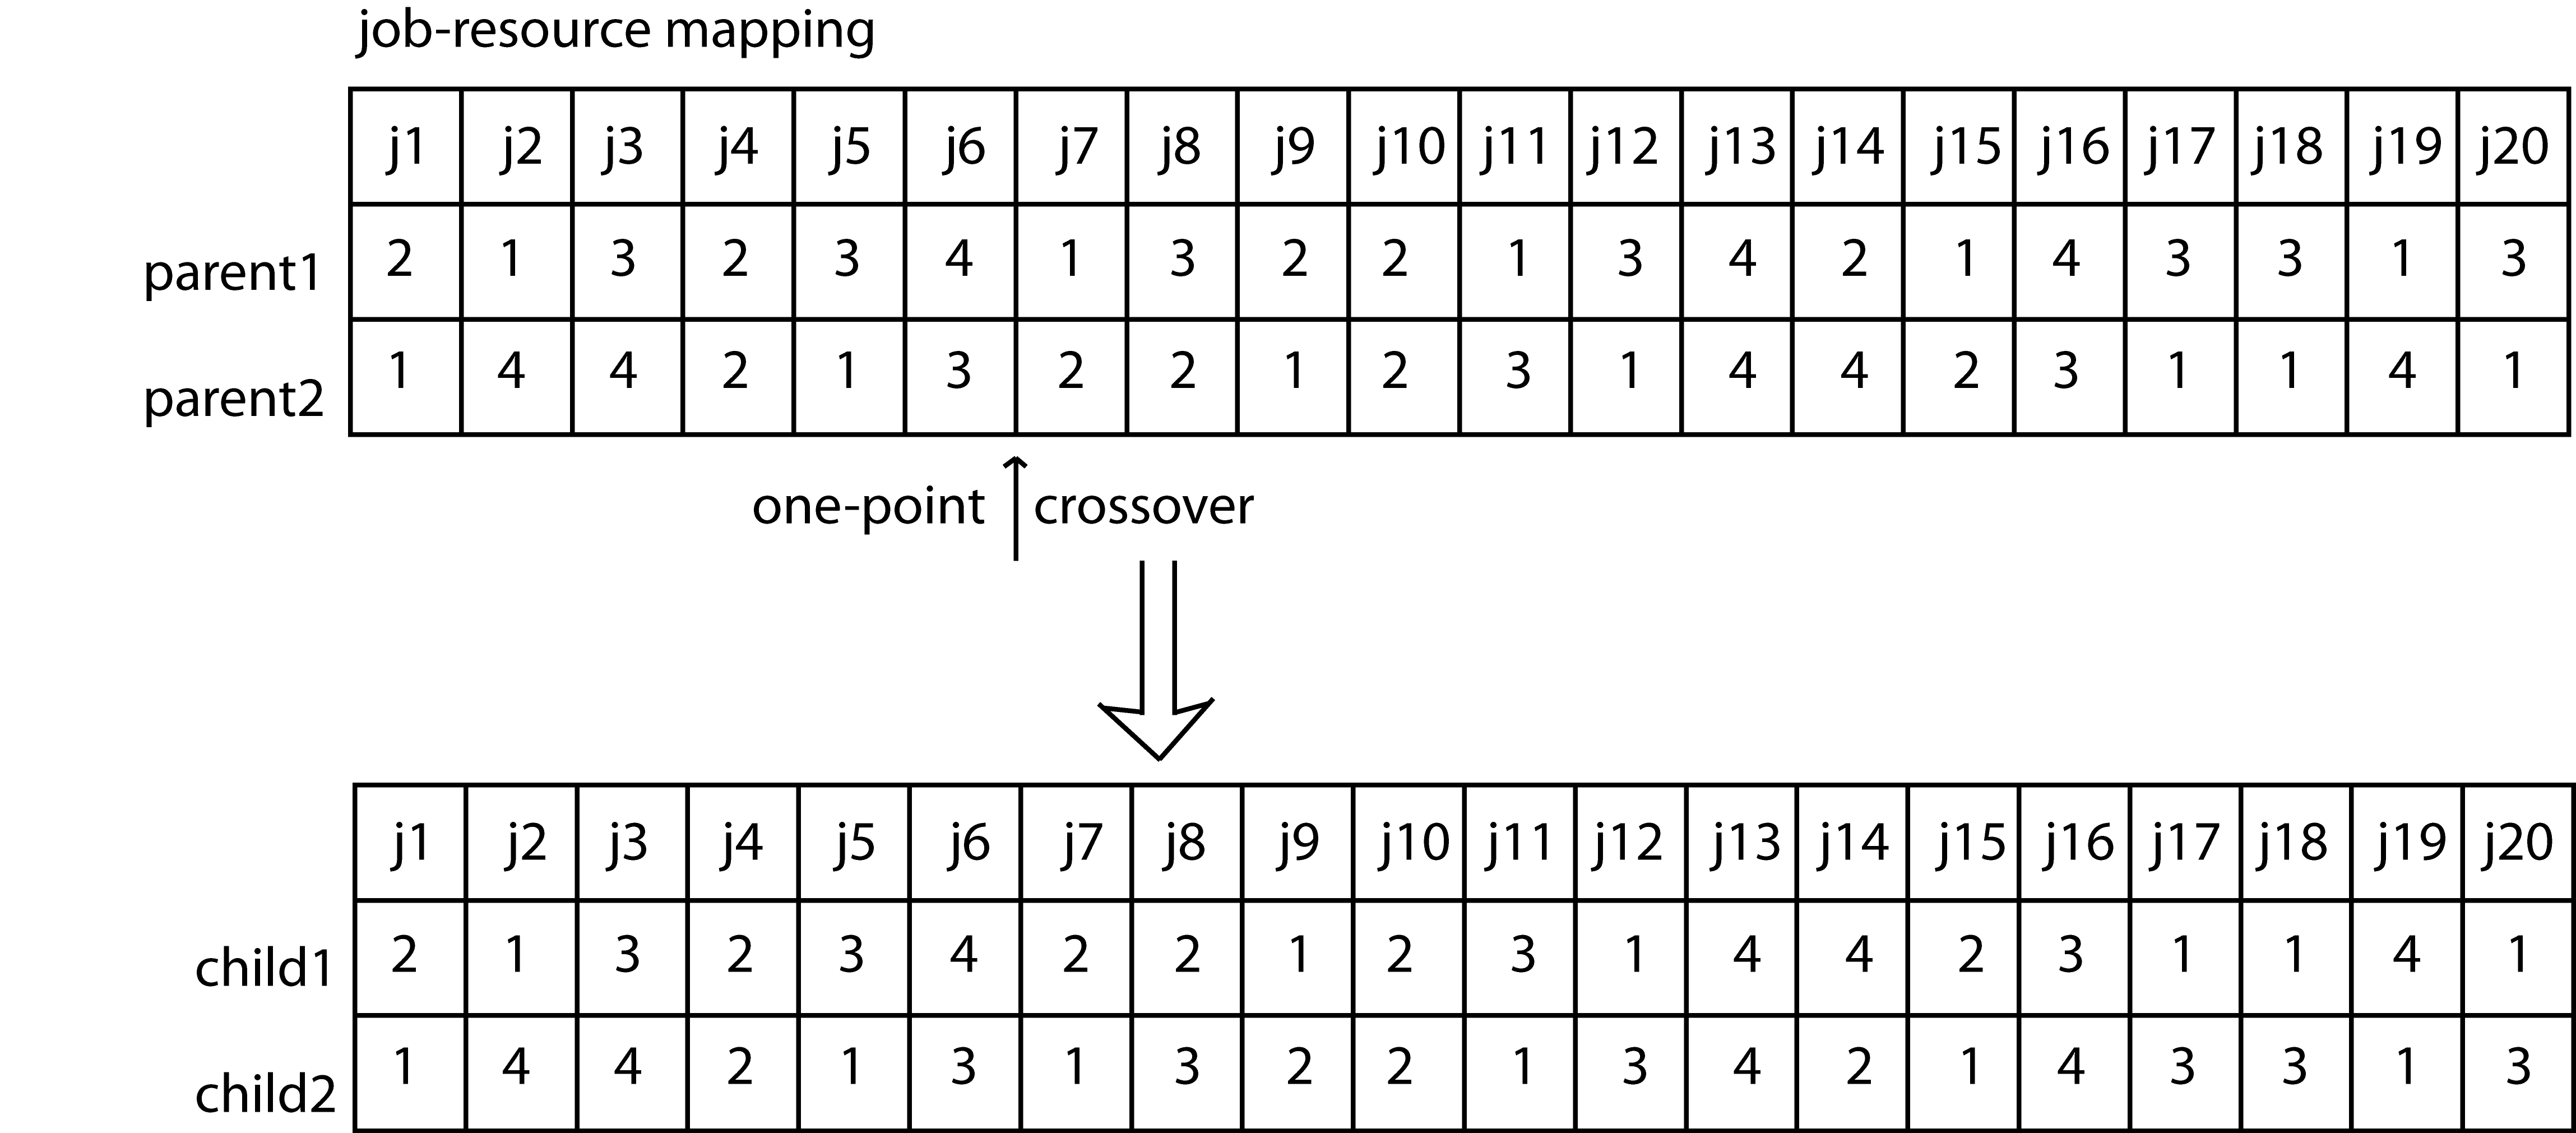
\includegraphics[width=1.0\columnwidth]{crossover1}
    \caption{One point crossover}
	\label{1pointxover}
\end{figure}
\begin{figure}[!h]
    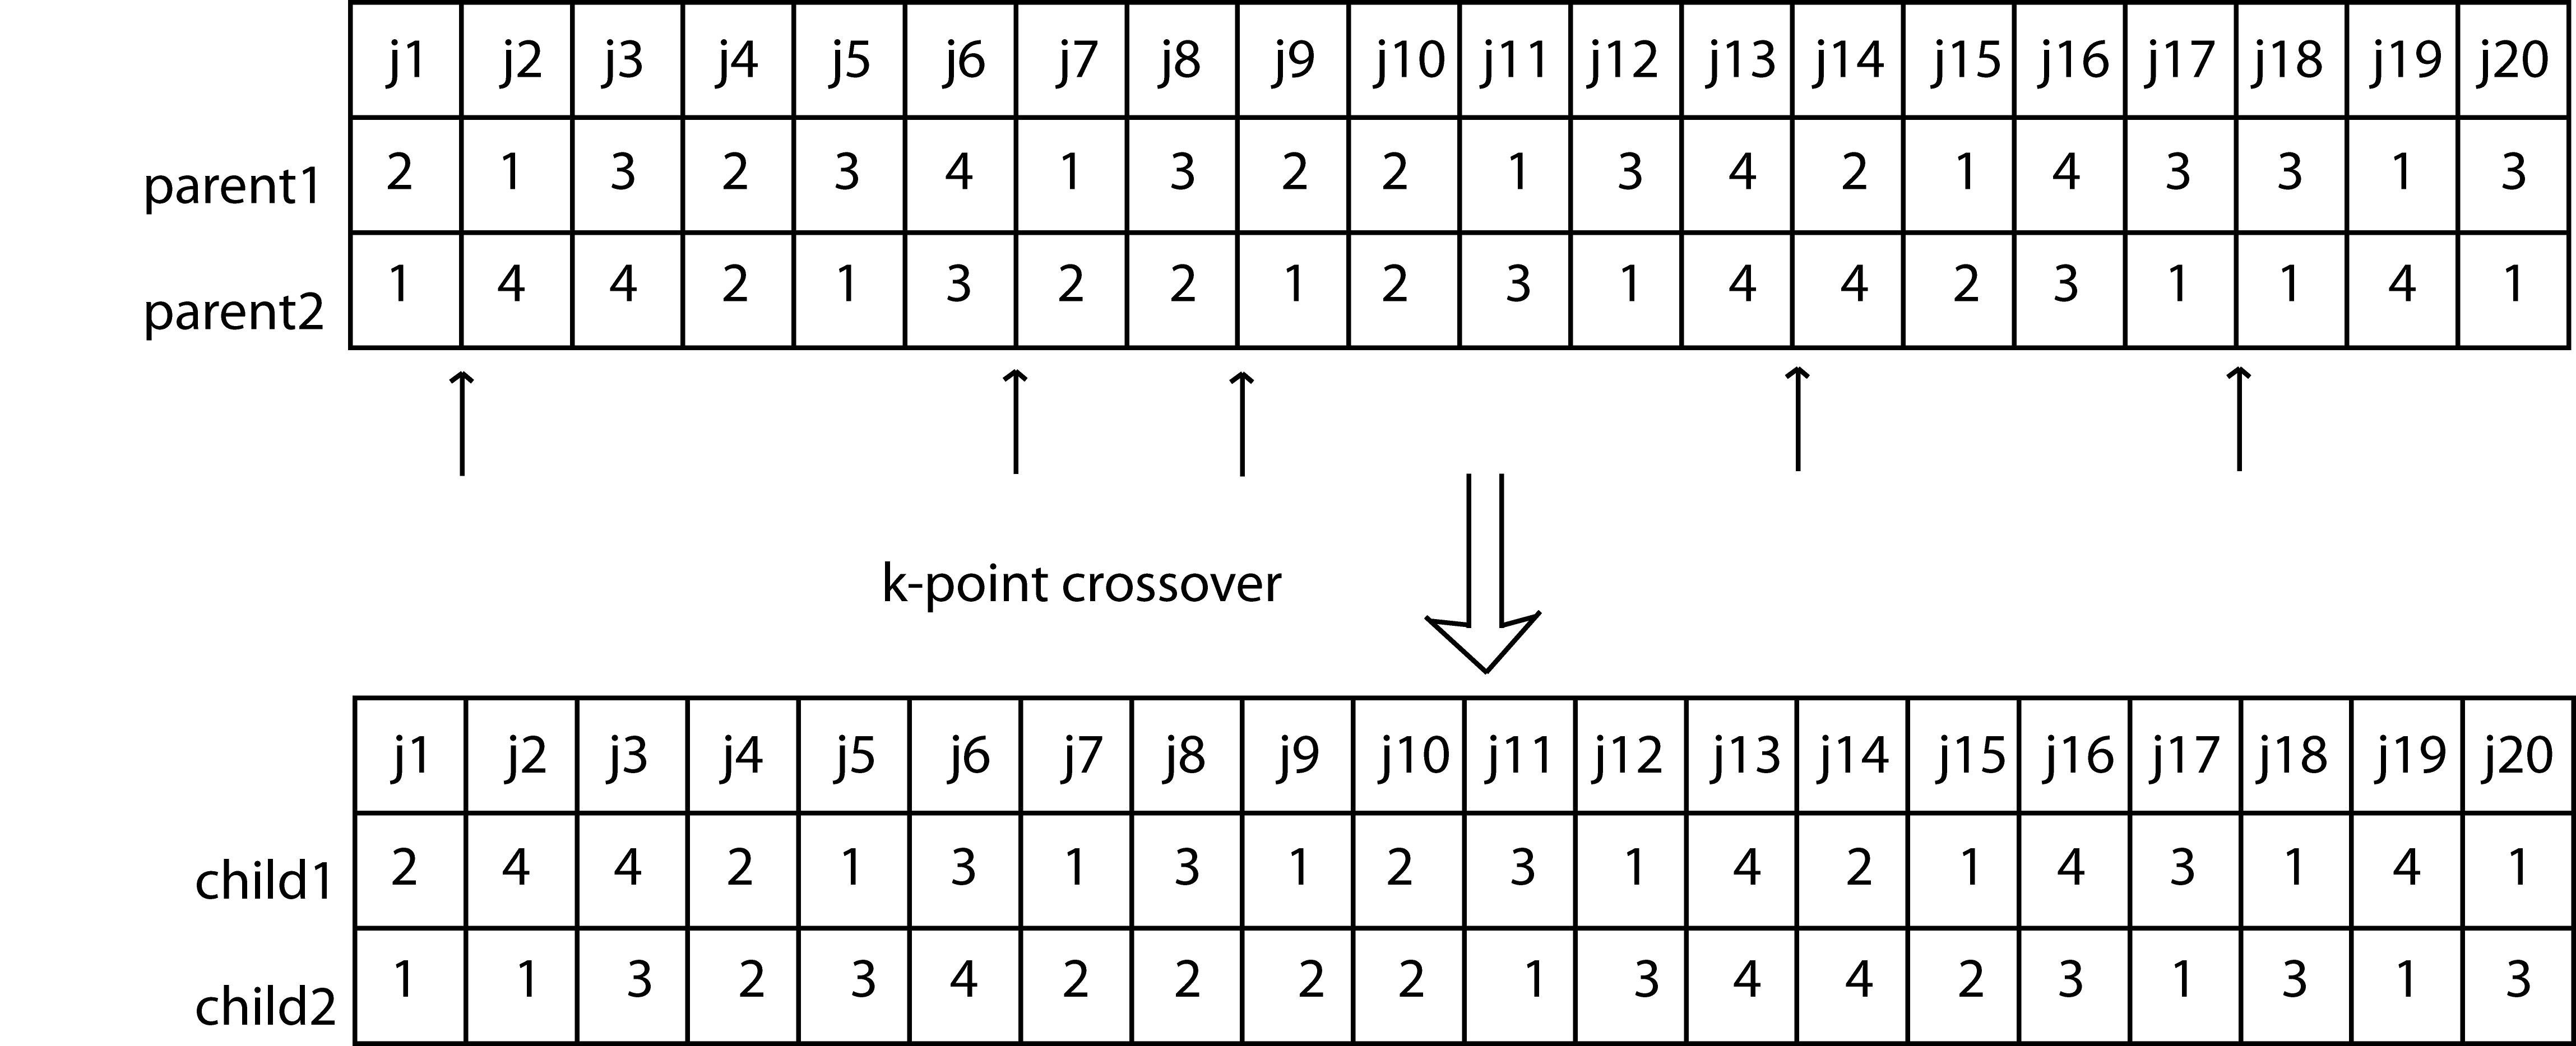
\includegraphics[width=1.0\columnwidth]{crossover2}
    \caption{k-point crossover}
	\label{kpointxover}
\end{figure}
\textbf{\emph{k-point crossover: }} This operator is a generalization of one-point crossover. Two or more cutting points i.e. $k \geq 2$ are randomly chosen and segments are interchanged alternately yielding two new descendants. However it should be noticed that large value of $k$ tends to explore more thoroughly the solution space but it is likely that it will destroy parents structure. An example is given in Figure ~\ref{kpointxover}.\\
\textbf{\emph{ Mask Crossover: }} A mask array of 0/1's is created randomly of size $NUM\_JOBS$ i.e. $mask = m_1,m_2,m_3,\ldots,m_{NUM\_JOBS}$ where $m_i = 0/1$. Figure ~\ref{mcrossover} explains this operator.
$$
\forall i, chromosome_{new_1}[i] = \left\{ \begin{array}{rl}
 chromosome_{parent_1}[i] &\mbox{ if $m_i = 0$} \\
 chromosome_{parent_2}[i] &\mbox{ otherwise}
       \end{array} \right.
$$
$$
\forall i, chromosome_{new_2}[i] = \left\{ \begin{array}{rl}
 chromosome_{parent_1}[i] &\mbox{ if $m_i = 1$} \\
 chromosome_{parent_2}[i] &\mbox{ otherwise}
       \end{array} \right.
$$
\begin{figure}[h]
    \centering
    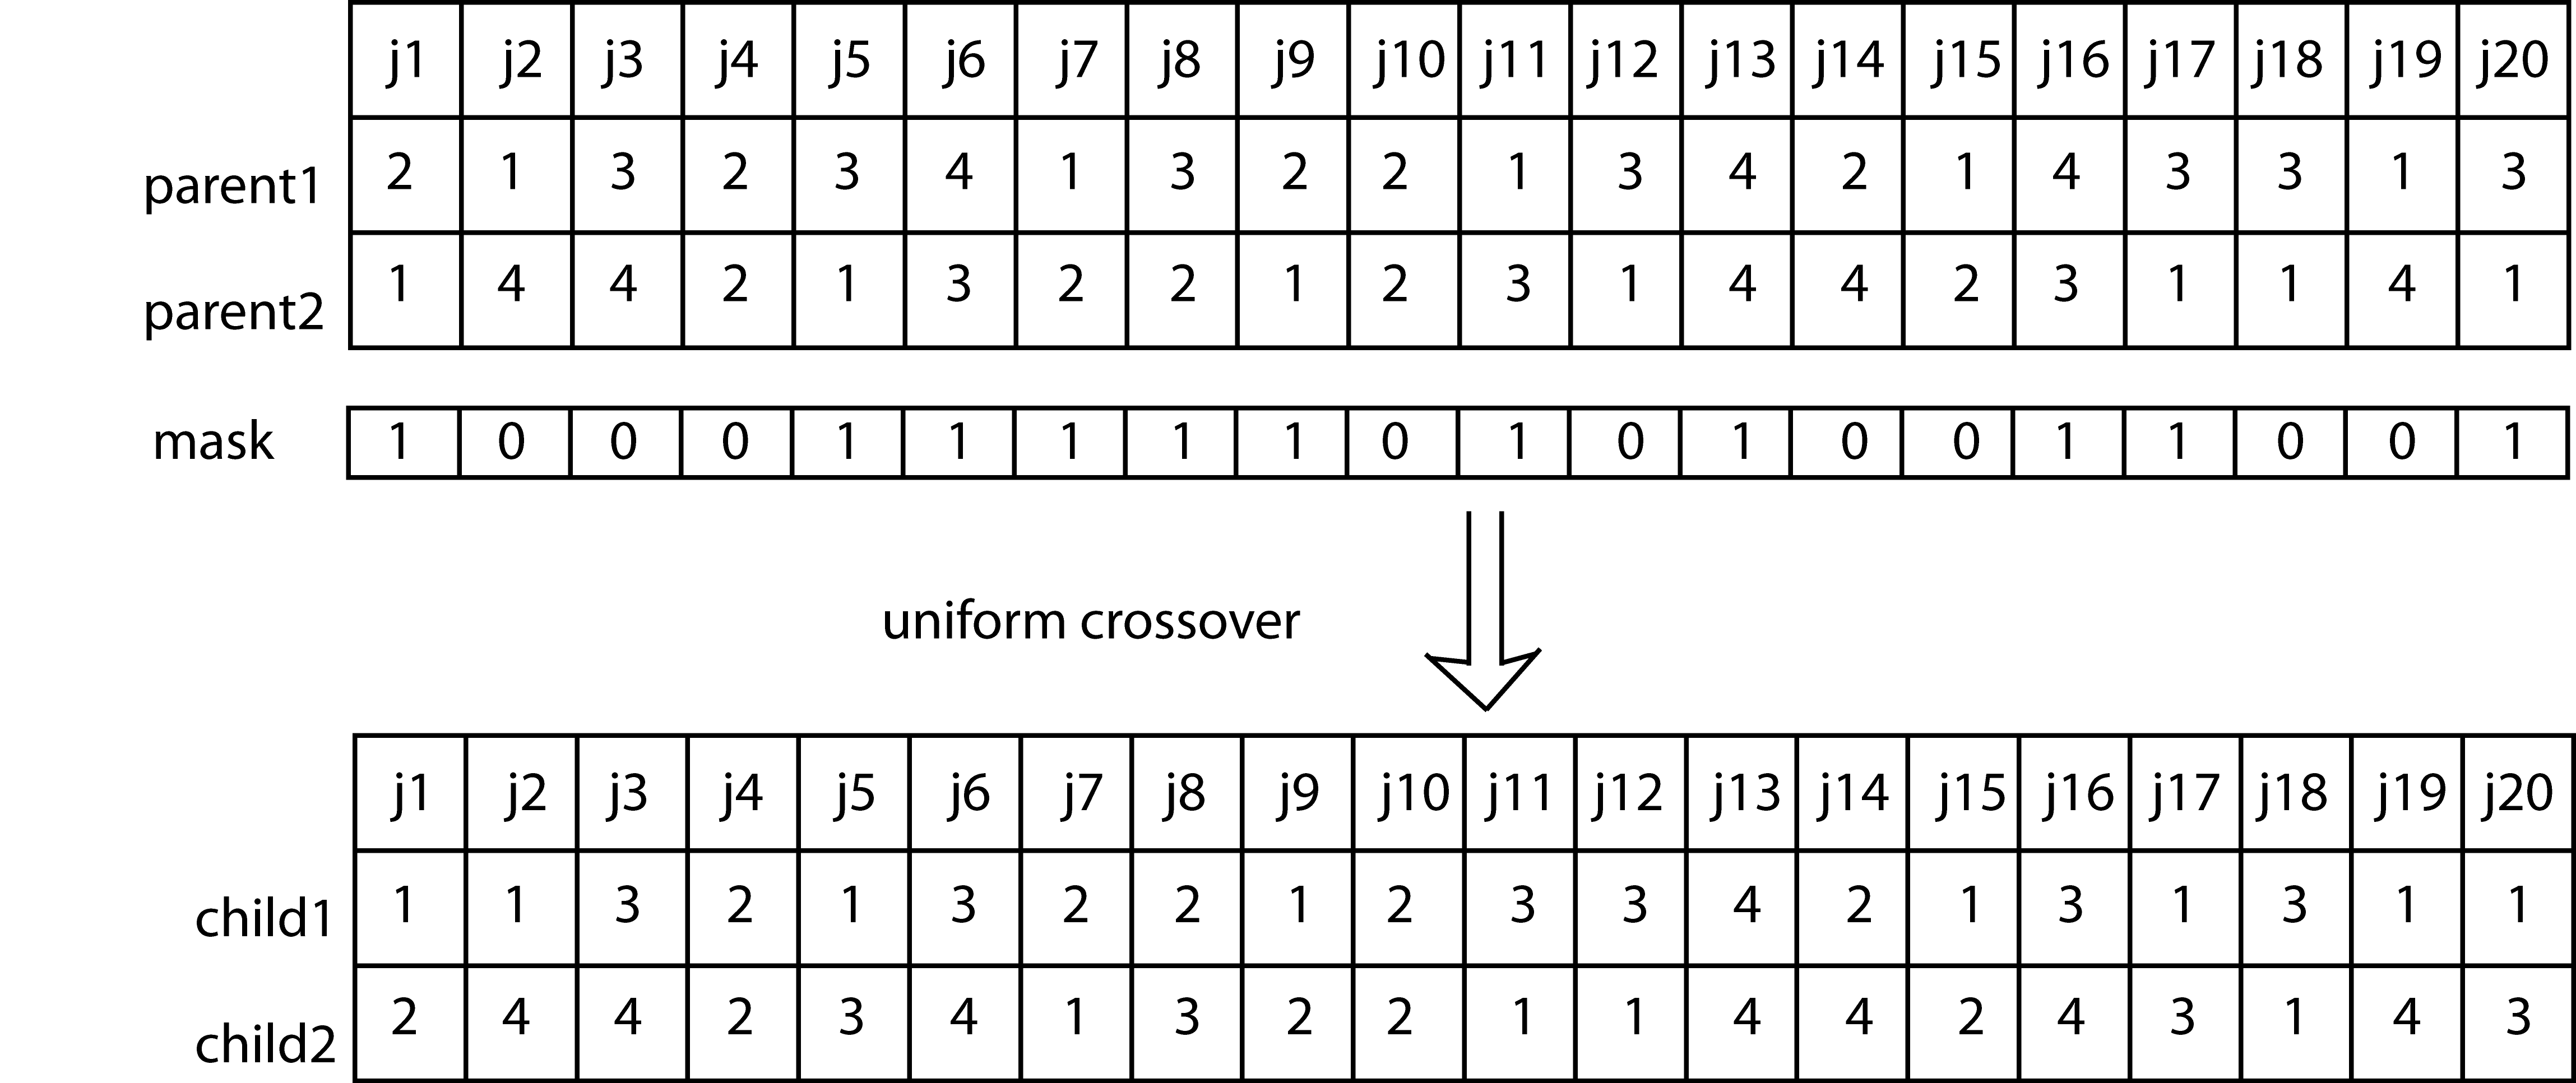
\includegraphics[width=1.0\columnwidth]{crossover3}
    \caption{Mask crossover}
	\label{mcrossover}
\end{figure}
\textbf{\emph{Fitness based Crossover: }} In this operator fitness or any other external function can be used. Our approach yield two descendants. The crossover is computed as follows. Working methodolgy can be inferred from Figure ~\ref{fitcrossover}.\\
$$
\forall i, chromosome_{new_1}[i] = \left\{ \begin{array}{rl}
 chromosome_{parent_1}[i] &\mbox{with probability $p = \frac{g_1[i]}{g_1[i] +g_2[i]}$} \\
 chromosome_{parent_2}[i] &\mbox{with probability $1-p$}
       \end{array} \right.
$$
$$
\forall i, chromosome_{new_2}[i] = \left\{ \begin{array}{rl}
 chromosome_{parent_1}[i] &\mbox{with probability $p = \frac{h_1[i]}{h_1[i] +h_2[i]}$} \\
 chromosome_{parent_2}[i] &\mbox{with probability $1-p$}
       \end{array} \right.
$$
\begin{figure}[t]
    \centering
    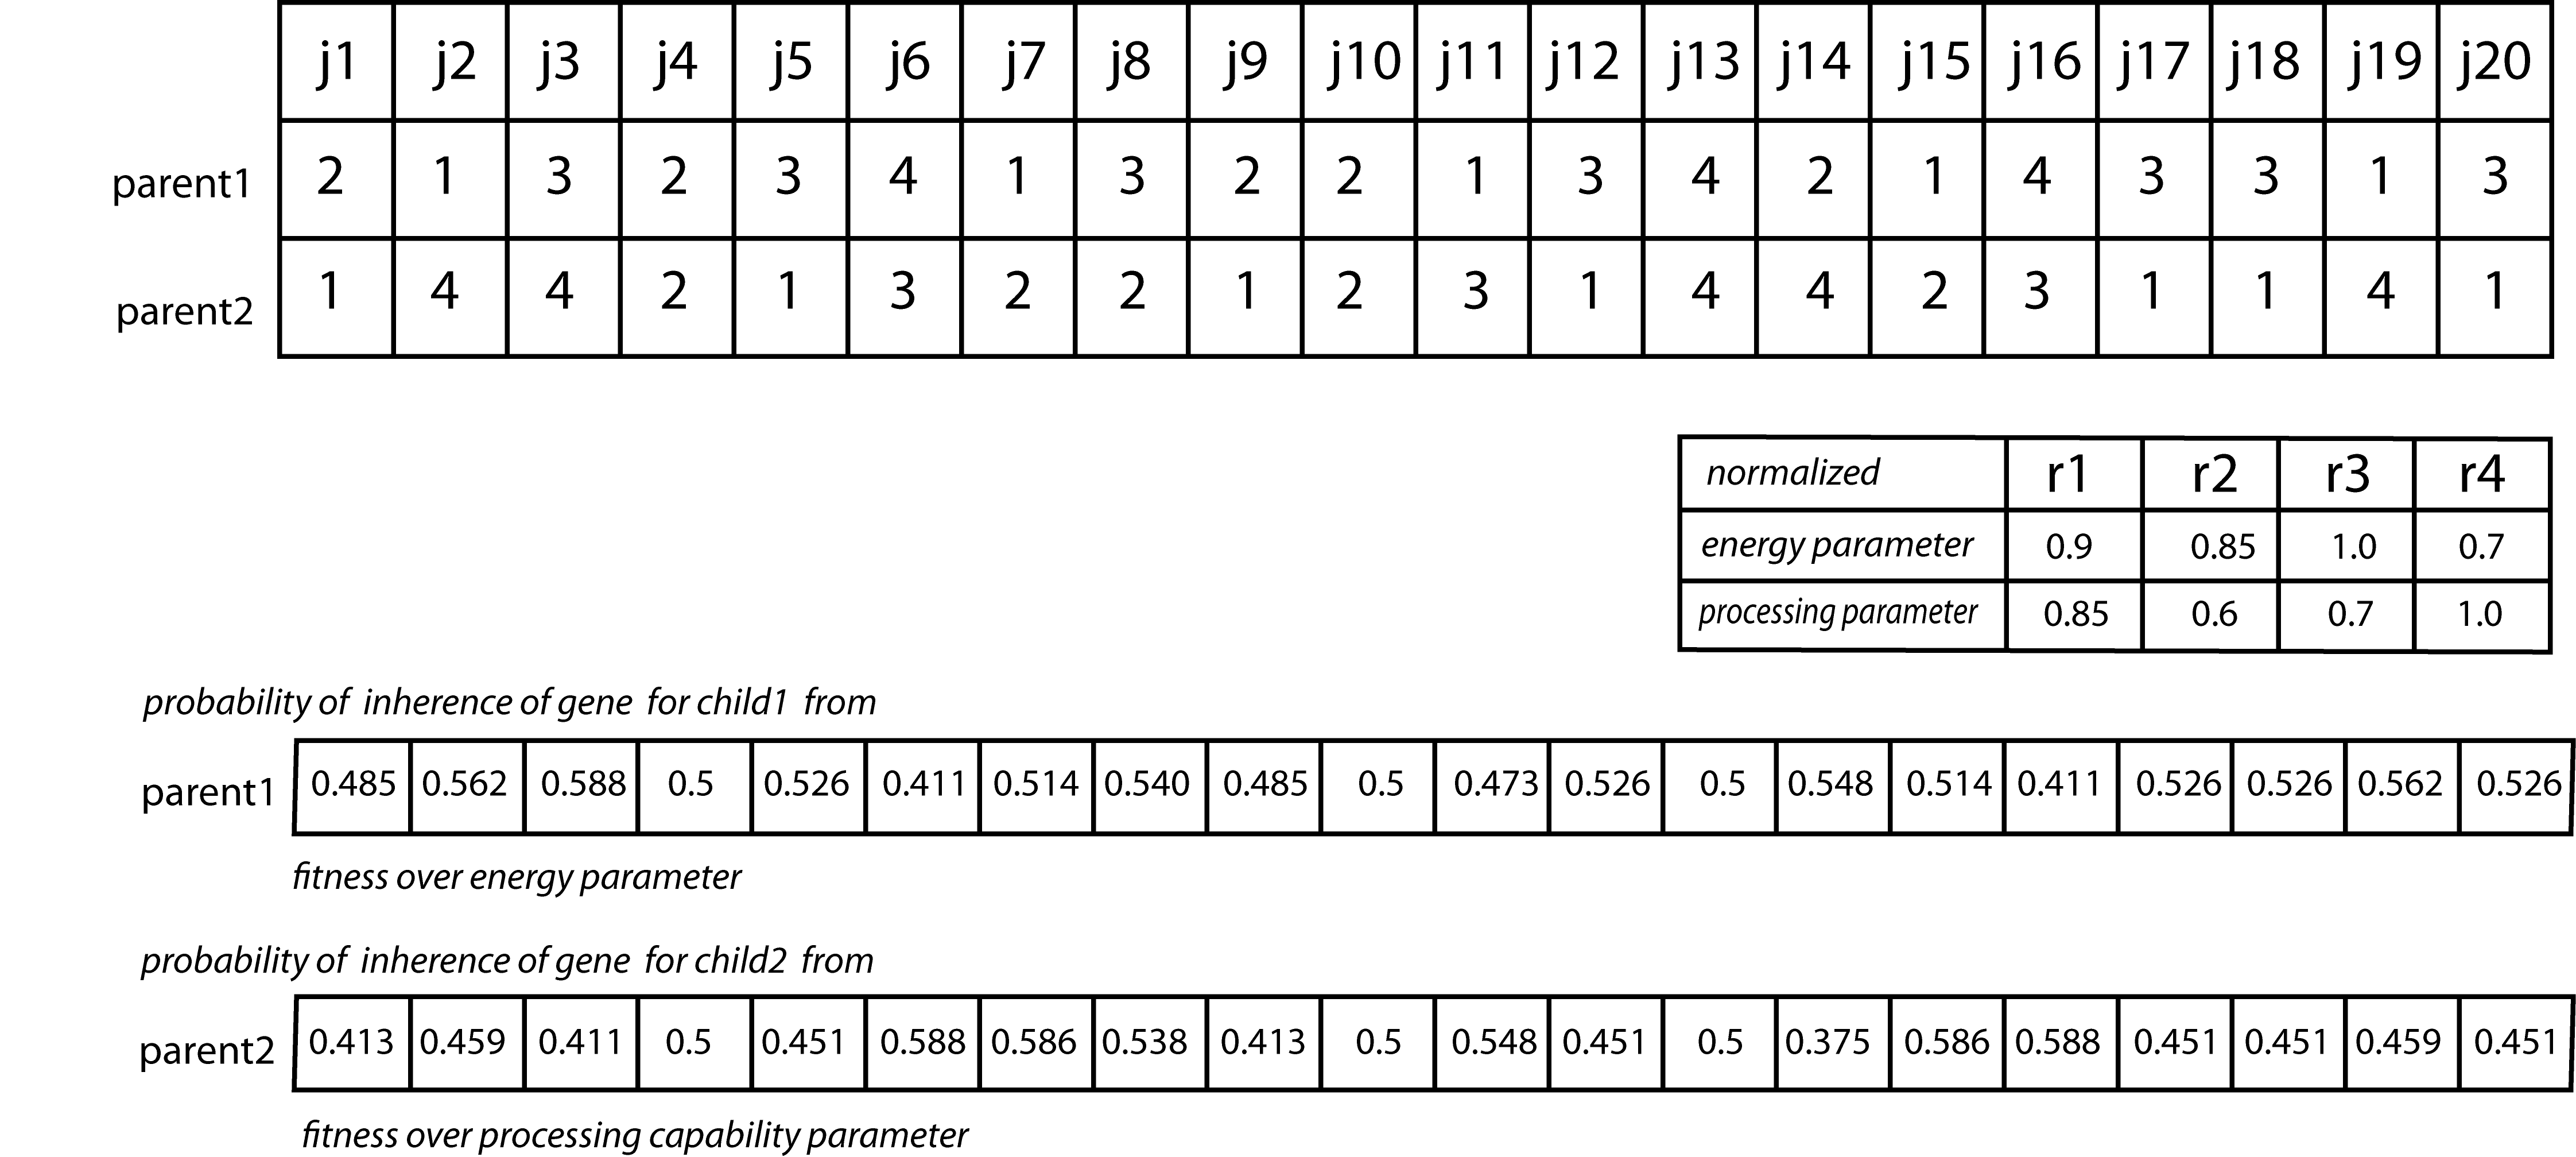
\includegraphics[width=1.0\columnwidth]{crossover5}
    \caption{Fitness based crossover}
	\label{fitcrossover}
\end{figure}
Each resource in grid has processing capability and energy efficiency parameter. They almost counteract each other and need a tradeoff between them to find optimal schedule.\\
Here  $g_1[i], g_2[i]$ are energy efficiency parameter of $chromosome_{parent_1}[i]$ and $chromosome_{parent_2}[i]$ respectively.
Similarly $h_1[i], h_2[i]$ are processing capability parameter of $chromosome_{parent_1}[i]$ and $chromosome_{parent_2}[i]$ respectively.
\subsubsection{Mutation}
$P_m$ is the probability with which mutation operator is applied. Mutation operators used as follows.\\
\textbf{\emph{ Move:}} This operator randomly assigns a resource to the job. Care is taken that resource type is same i.e. resource belongs to same set.\\
\textbf{\emph{ Swap:}} This operator randomly chooses two jobs and swap their assigned resources if they belong to same set.\\
\textbf{\emph{ Rebalancing: }} This operator takes into account number of jobs assigned to each resource. This operator chooses most overloaded resource and randomly pick a job assigned to it. Then the job is moved to a resource which is less overloaded.\\
\begin{figure}[ht]
    \centering
    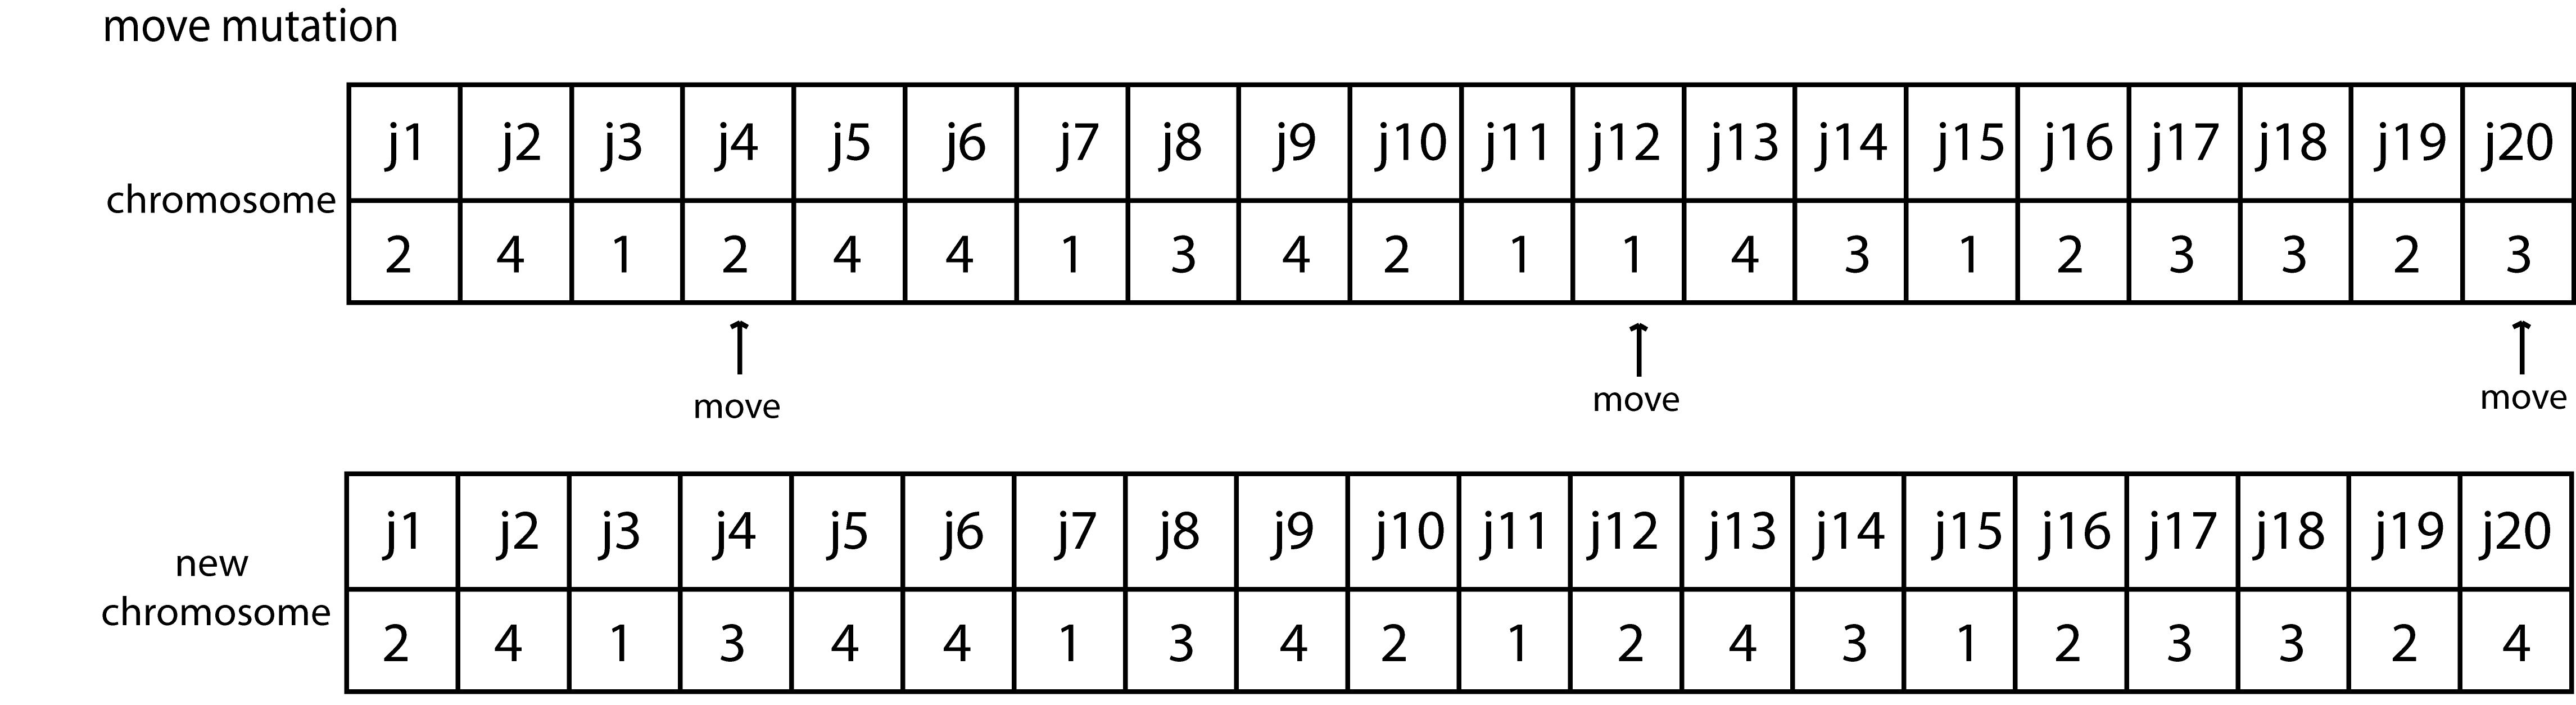
\includegraphics[width=1.0\columnwidth]{mutation1}
    \caption{Mutation- move}
	\label{movemuta}
\end{figure}
\begin{figure}[h]
    \centering
    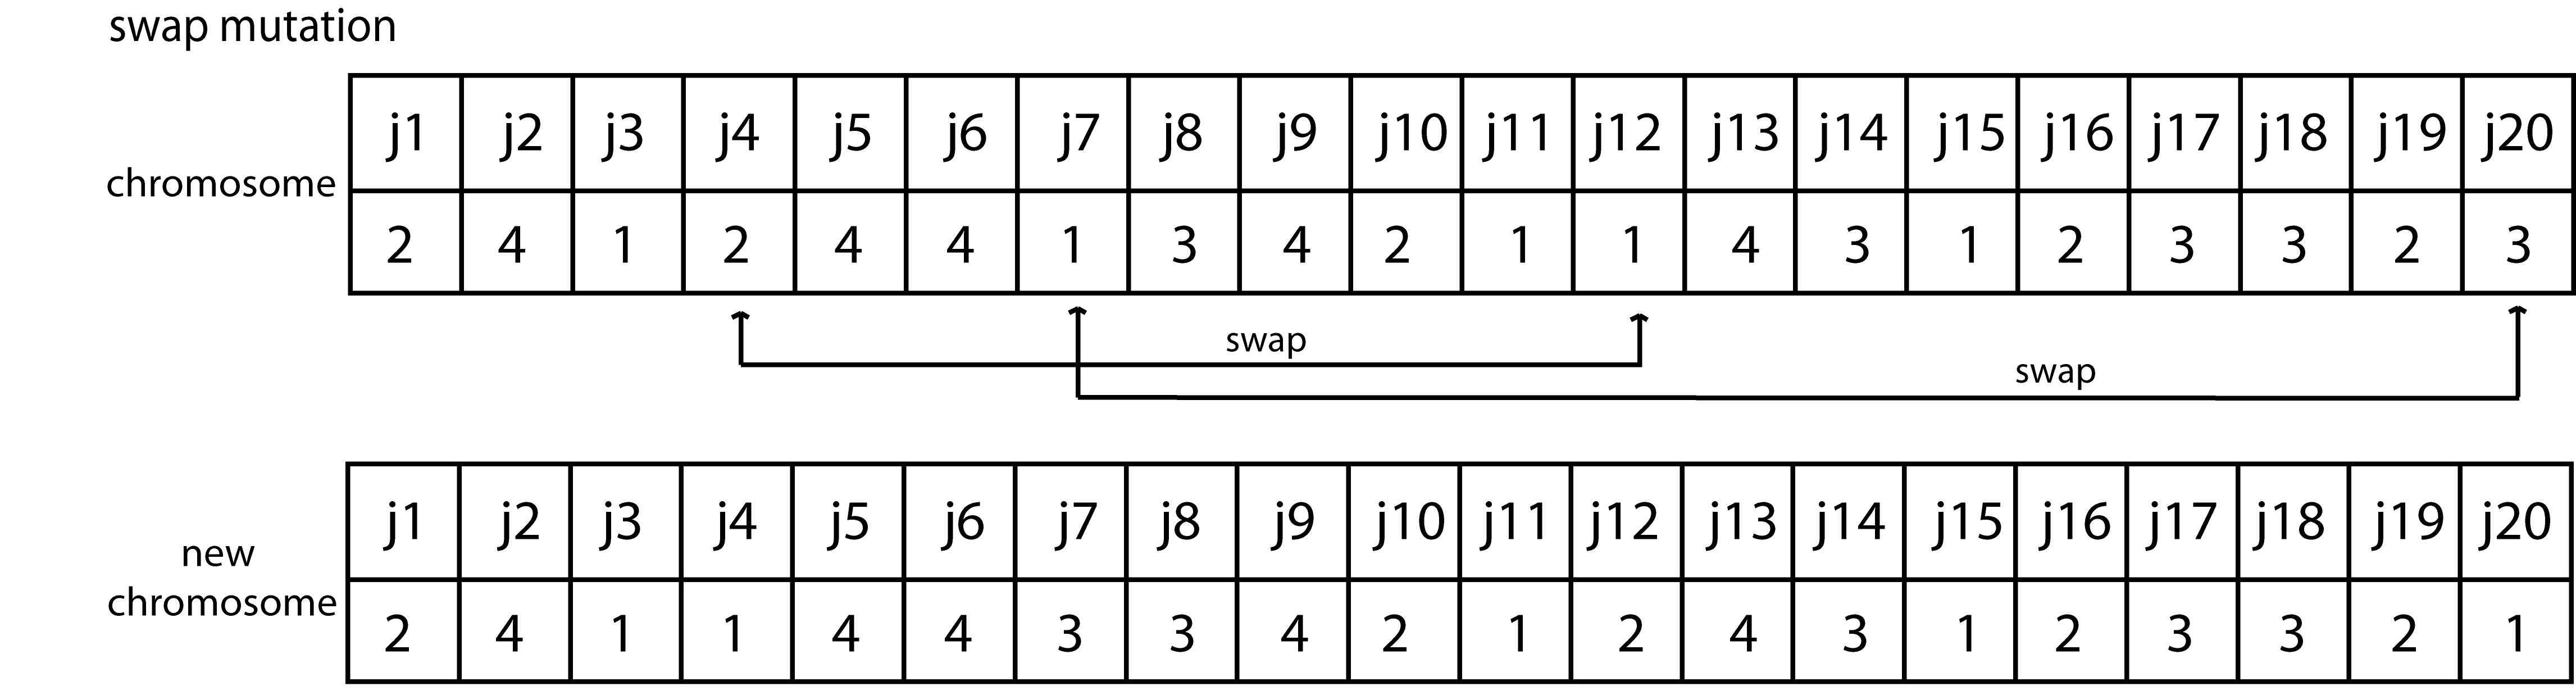
\includegraphics[width=1.0\columnwidth]{mutation2}
    \caption{Mutation- swap}
	\label{swapmuta}
\end{figure}
\subsubsection{Elitism}
In the process of crossover and mutation it is possible that some good chromosomes might be lost. Elitism is a mechanism to preserve these chromosomes. A small percentage of the fittest population i.e. first pareto front in multi-objective search space is forwarded to be the part of new population for next iteration.
\section{Dynamic scheduling}
\label{dynamicscheduling}
Application jobs queued in grid are fed to the MOJS module in batch. The output is the elitist pareto front of chromosomes comprises near optimal schedules. Soft constraints and weighted sum approach is applied on multiple objectives to finalize a chromosome as scheduling strategy. Some jobs are queued on their respective resource while others are again fed to MOJS module. The number of jobs queued depend on the fitness of the chromosome and time available for the scheduler to re-run and find a better schedule. Progress is ensured by setting a minimum number of jobs to be queued on a single run of module. \\
As this is a real time scheduling problem and resources are dynamic in nature it can participate and leave the system any time, it is of higher importance to make the scheduling dynamic in nature. By dynamic we mean re-allocation of already scheduled jobs which were not completed. So change in the resource pool can trigger running of scheduler which can either reschedule the jobs whose resources have left the grid or can request processing of new jobs on addition of one or more resources or both of them. Jobs whose predecessors is present in the set of rescheduled jobs are also rescheduled. \\
There is very little scope for this paper to solve the issue where a job suffers starvation and penalty due to failure of resource. To handle this issue accounting of Mean Time to Failure (MTTF) with log mining can help.
\section{Job Grouping for Fine-grained Jobs}
\label{jobgr}
Fine grained jobs are grouped to form a single job. Following are the constraints considered while job grouping.
\begin{itemize}
 \item Jobs grouped as single job should be of same type i.e. either computational jobs or storage intensive jobs. 
 \item Prevail same job precedence rule after job grouping.
\end{itemize}
Workflow and precedence of jobs is represented through Directed Acyclic Graph (DAG), where nodes are jobs and directed edge represents precedence. \\
A directed edge from $a$ to $b$ is drawn, when $b$ awaits for the completion of job $a$ and $a$ is said to be the predecessor of $b$ and $b$ is the successor of $a$. Nodes having common edge are defined as adjacent nodes. We define $a,b$ to have same job type if their resource type requirement is same.\\
Before we present our heuristic algorithm for job-grouping, we define few terms as follows:
\subsection{Entry job}
A job without any predecessor but has atleast one successor is called entry job. If there are multiple entry jobs for a DAG component then we add a zero size job/node and new directed edges are drawn from zero size job to entry jobs. Hence we have a single entry job denoted as $j_{entry}$.
\subsection{Exit job}
A job without any successor but has atleast one predecessor is called exit job. If there are multiple exit jobs for a DAG component then we add a zero size job/node and new directed edges are drawn from  exit jobs to zero size job. Hence we have a single exit job denoted as $j_{exit}$.
\subsection{Job size}
Size of a computational job is measured in Million Instructions(MI) and storage jobs in Megabytes(MB). It is denoted as $job\_size(j)_{computational}$ or $job\_size(j)_{storage}$. 

\begin{framed}
{\small
\emph{Note:}
\begin{itemize}
\item A computational job has $job\_size(j)_{storage} =0$ MB
\item A storage job has $job\_size(j)_{computational}=0$ MI
\end{itemize}
}
\end{framed}

\begin{algorithm}[ht]
\caption{job grouping}
\begin{algorithmic}
\REQUIRE { Job pool with DAG representation }
\STATE {Compute $crit_{up}(j)_{<type>}$ for each job $j$   according to the equation ~\ref{eq:up1} }
\STATE {Compute $crit_{down}(j)_{<type>}$ for each job $j$ according to the equation ~\ref{eq:down1} }
\STATE { Compute $crit_{<type>}$ for each job $j$  according to the equation ~\ref{eq:cr} }
\WHILE { Job $a \in $ job pool exists, where $a$ is unprocessed fine-grained job }
  \STATE { $flag \leftarrow 0$ }
  \WHILE { $a$ is fine-grained job \AND $flag = 0$ }
    \FOR {each $b \in adjacent\_node(a)$ \AND  same type i.e. computational or storage }
	  \STATE { Temporary merge adjacent node $b$ and $a$ to form $t$}
	  \STATE { Calculate new $crit_{up}(t)_{<type>}$ , $crit_{down}(t)_{<type>}$ and $crit(t)_{<type>}$ }
	  \IF {new $crit(t)_{<type>} \leq crit(j_{entry})_{<type>}$ \AND $crit(t)_{<type>}$ is minimum till now }
	      \STATE { $merge\_node$ $\leftarrow b$ }
	  \ENDIF
    \ENDFOR
    \IF { $merge\_node$ is found }
	\STATE { Permanently merge $merge\_node$ with $a$ to form $a'$ }
	\STATE Change parent and child relation accordingly 
	\IF { $a'$ is not fine-grained job}
	    \STATE { $flag\leftarrow 1$ }
	\ENDIF
    \ELSE 
	    \STATE { $flag\leftarrow 1$ }
    \ENDIF
\ENDWHILE
\ENDWHILE
\end{algorithmic}
\label{jobgrouping}
\end{algorithm}

\subsection{Critical length }
Critical length denoted as $crit(j)$ refers to the longest distance from $j_{entry}$ to $j_{exit}$ passing through the job $j$. There are two types of jobs viz., computational intensive and storage intensive jobs. Hence we consider $crit(j)_{computational}$, $crit(j)_{storage}$ accordingly for calculation in Algorithm~\ref{jobgrouping} depending on the job type.\\
The Upward Critical length of job $j$ is the longest distance from $j$ to the exit job $j_{exit}$. It is denoted as $crit_{up}(j)_{<type>}$ where $_{<type>}$ is computational and storage. Upward critical length is computed with the equation~\ref{eq:up1} starting from $j{exit}$ and moving upward towards $j$.
\begin{equation}\label{eq:up1}
crit_{up}(j)_{<type>} = job\_size(j)_{<type>} + max_{j' \in succ(j)}(crit_{up}(j')_{<type>})
\end{equation}
%\begin{equation}\label{eq:up2}
%crit_{up}(j)_{storage} = job\_size(j)_{storage} + max_{j' \in succ(j)}(crit_{up}(j')_{storage})
% \end{equation}
Similarly, the Downward Critical length of job $j$ is the longest distance from the entry job $j_{entry}$ to $j$. It is denoted as $crit_{down}(j)_{<type>}$ where $_{<type>}$ is computational and storage. Downward critical length is computed with the equation~\ref{eq:down1} starting from $j{entry}$ and moving downward towards $j$.
\begin{equation}\label{eq:down1}
crit_{down}(j)_{<type>} = job\_size(j)_{<type>} + max_{j' \in pred(j)}(crit_{down}(j')_{<type>}) 
\end{equation}
%\begin{equation}\label{eq:down2}
%crit_{down}(j)_{storage} = job\_size(j)_{storage} + max_{j' \in pred(j)}(crit_{down}(j')_{storage}) 
%\end{equation}
\begin{equation}\label{eq:cr}
crit(j)_{<type>} = crit_{up}(j)_{<type>} + crit_{down}(j)_{<type>}
\end{equation}
\begin{framed}
{\small \emph{Note:} $crit(j_{entry})_{<type>}$ is the longest distance from $j_{entry}$ to $j_{exit}$ in the DAG. The path with the longest distance from the $j_{entry}$ to $j_{exit}$ is called \emph{critical path}. Any job whose $crit(j)_{<type>}$ value is equal to $crit(j_{entry})_{<type>}$ is on a critical path is considered as a critical job. The heuristic applied in algorithm~\ref{jobgrouping} is to group fine-grained jobs without increasing the critical path length of the DAG.}
\end{framed}

\section{Algorithm Description}
\begin{algorithm}[!h]
\caption{MOJScheduler}
\label{MOJScheduler}
\begin{algorithmic}
\REQUIRE {Jobs[$NUM\_JOBS$],Resource[$NUM\_RESOURCES$],$n$,$num\_iteration$}
    \STATE {Initialization: Generate initial population $ P_0 $ of  $n$ chromosomes}
    \STATE {Fitness Calculation: }
    \FOR {$i = 1 \to n$} 
	\STATE {Evaluate(chromosome[i] from $P_i$)}
    \ENDFOR
    \FOR {$i = 1 \to num_iteration$}
      \STATE {Selection: Select a subset of even number of chromosomes from $P_i$}
      \STATE {$P_{i_1} = Select(P_i)$}
      \STATE {Crossover: With probability $P_c$ crossover every two chromosome from $P_{i_1}$}
      \STATE {$P_{i_2} = crossover(P_{i_1})$}
      \STATE {Mutation: With probability $P_m$ mutate chromosome from $P_{i_2}$}
      \STATE {$P_{i_3} = mutate(P_{i_2})$}
      \STATE {Fitness Calculation: }
	  \FOR {$i = 1 \to n$} 
	    \STATE {Evaluate(chromosome[i] from $P_{i_3}$)}
	  \ENDFOR
      \STATE {$P_{i_4} = P_i + P_{i_3}$}
      \STATE {Assign non-domination rank to each chromosome, Non-dominating\_Sort($P_{i_4}$)}
      \STATE {calculate\_crowding\_distance($P_{i_4}$)}
      \STATE {Sort based on Crowding distance of each chromosome}
      \STATE {crowding\_distance\_sorting($P_{i_4}$)}
      \STATE {Replacement: Create population for new generation}
      \STATE {Forward 1st $n$ chromosomes from sorted set $P_{i_4}$ to $P_{i+1}$}
     \ENDFOR
  \RETURN{Chromosomes with non-domination rank 1 i.e. First pareto front}
%  \end{pseudocode}
\end{algorithmic}
\end{algorithm}


\begin{algorithm}[ht]
\caption{crossover($P_i$)}
\label{crossover}
\begin{algorithmic}
\REQUIRE {Set of chromosomes $P_i$ with population $2m$,$P_c$}
\STATE Initialize set $Q$
    \FOR {$i = 1 \to m$}
	\STATE {Randomly choose two chromosome $x,y$ from $P_i$}
	\STATE $p= random\_double(0,1)$, $random\_double(x,y)$ generates a number $[x,y]$
	\IF{ $p < p_c$} 
	  \STATE {$c = random\_int(0,2)$, $random\_int(x,y)$ generates an integer $[x,y]$}
	   \IF {$c =0$}
		\STATE { $k \leftarrow random\_int(0,10)$ }
		\STATE { $x_1,y_1 = k\_point\_crossover(x,y)$ }
		\STATE {Add $x_1,y_1$ to $Q$}
	  \ENDIF
	  \IF{$c =1$}
		 \STATE { $x_1,y_1 \leftarrow uniform\_crossover(x,y)$ }
		 \STATE {Add $x_1,y_1$ to $Q$}
	  \ENDIF
	  \IF{$c =2$}
		\STATE { $x_1,y_1 \leftarrow fitness\_based\_crossover(x,y)$ }
		\STATE {Add $x_1,y_1$ to $Q$}
	  \ENDIF
	\ENDIF
    \ENDFOR
  \RETURN{Set $Q$}
%  \end{pseudocode}
\end{algorithmic}
\end{algorithm}


\begin{algorithm}[!ht]
\caption{mutation($P_i$)}
\label{mutation}
\begin{algorithmic}
\REQUIRE {Set of chromosomes $P_i$, $P_m$}
    \FOR {$i = 1 \to $ size($P_i$)}
	\STATE Select $chromosome[i]$
	\STATE $p= random\_double(0,1)$, $random\_double(x,y)$ generates a number $[x,y]$
	\IF{ $p < p_m$} 
	  \STATE {$c = random\_int(0,2)$, $random\_int(x,y)$ generates an integer $[x,y]$}
	   \IF {$c =0$}
	      \STATE {$count = random\_int(1,10)$, change at most 10 genes}
	      \FOR{$i = 1 \to count$ }
		\STATE { $pos = random\_int(0,NUM\_JOBS)$ }
		\STATE { Assign a new resource to gene $pos$ from same resource type}
		\STATE { $move(chromosome[i]$,$pos$) }
	      \ENDFOR
	   \ENDIF
	   \IF {$c =1$}
	      \STATE {$count = random\_int(1,10)$, change at most 10 genes}
	      \FOR{$i = 1 \to count$ }
		\STATE { $pos_1 = random\_int(0,NUM\_JOBS)$ }
		\STATE { $pos_2 = random\_int(0,NUM\_JOBS)$ }
		\STATE { Assign a new resource to gene $pos$ from same resource type}
		\STATE { $swap(chromosome[i]$,$pos_1$,$pos_2)$ }
	      \ENDFOR
	   \ENDIF
	   \IF {$c =2$}
	      \STATE {$count = random\_int(1,10)$, change at most 10 genes}
	      \FOR{$i = 1 \to count$ }
		\STATE { $pos = random\_int(0,NUM\_JOBS)$ }
		\STATE { Assign a new resource to gene $pos$ from same resource type}
		\STATE { $rebalancing(chromosome[i]$,$pos$) }
	      \ENDFOR
	   \ENDIF
	\ENDIF
    \ENDFOR
  \RETURN{Set $P_i$}
%  \end{pseudocode}
\end{algorithmic}
\end{algorithm}


\begin{algorithm}[!ht]
\caption{calculate\_crowding\_distance($P_i$)}
\label{mutation}
\begin{algorithmic}
\REQUIRE {Set of chromosomes $P_i$}
    \STATE $l = size(P_i)$
    \FOR {$i = 1 \to l$}
      \STATE $dist_{chromosome[i]} = 0$
    \ENDFOR
    \FOR {$m = 1 \to num\_obj $, Here number of objective i.e. $num\_obj$ functions is 5 }
    \STATE { sort($P_i$,$m$) }
    \STATE { $dist_{chromosome[1]} \leftarrow \infty $ }
    \STATE { $dist_{chromosome[l]} \leftarrow \infty $, ensuring boundary chromosomes are always there }
      \FOR {$i = 2 \to l-1$}
	\STATE $dist_{chromosome[i]}= dist_{chromosome[i]} + \frac{f_{chromosome[i+1]_m} - f_{chromosome[i-1]_m}}{f_m^{max} -f_m^{min}}$
	\STATE where $f_{chromosome[i]_m}$ is $m$th objective function of $chromosome[i]$ 
	\STATE  $f_m^{max}$ is max value of $m$th objective function \&
	\STATE $f_m^{min}$ is min value of $m$th objective function
      \ENDFOR
    \ENDFOR
  \RETURN{Set $P_i$}
%  \end{pseudocode}
\end{algorithmic}
\end{algorithm}


        \chapter{Implementation  and Results}
We have implemented our proposed scheduler and simulated the grid environment with standard worloads. The dispatcher uses Message Passing Interface(MPI) communication environment to interact with the resources and submit jobs. In this chapter implementation methods and experimentation details of scheduler and its performance based on various parameters have been discussed.
\section{Implementation Details}
We have implemented our work in C++ programming language. The job scheduler module schedule jobs. The resource manager simulates the dynamic behaviour of resources in grid. An initial configuration of the online resources is considered before starting the job scheduling process. The dispatcher send jobs to corresponding resources.\\
Implemented system with job scheduler module has following features.
\begin{figure}[t]
    \centering
    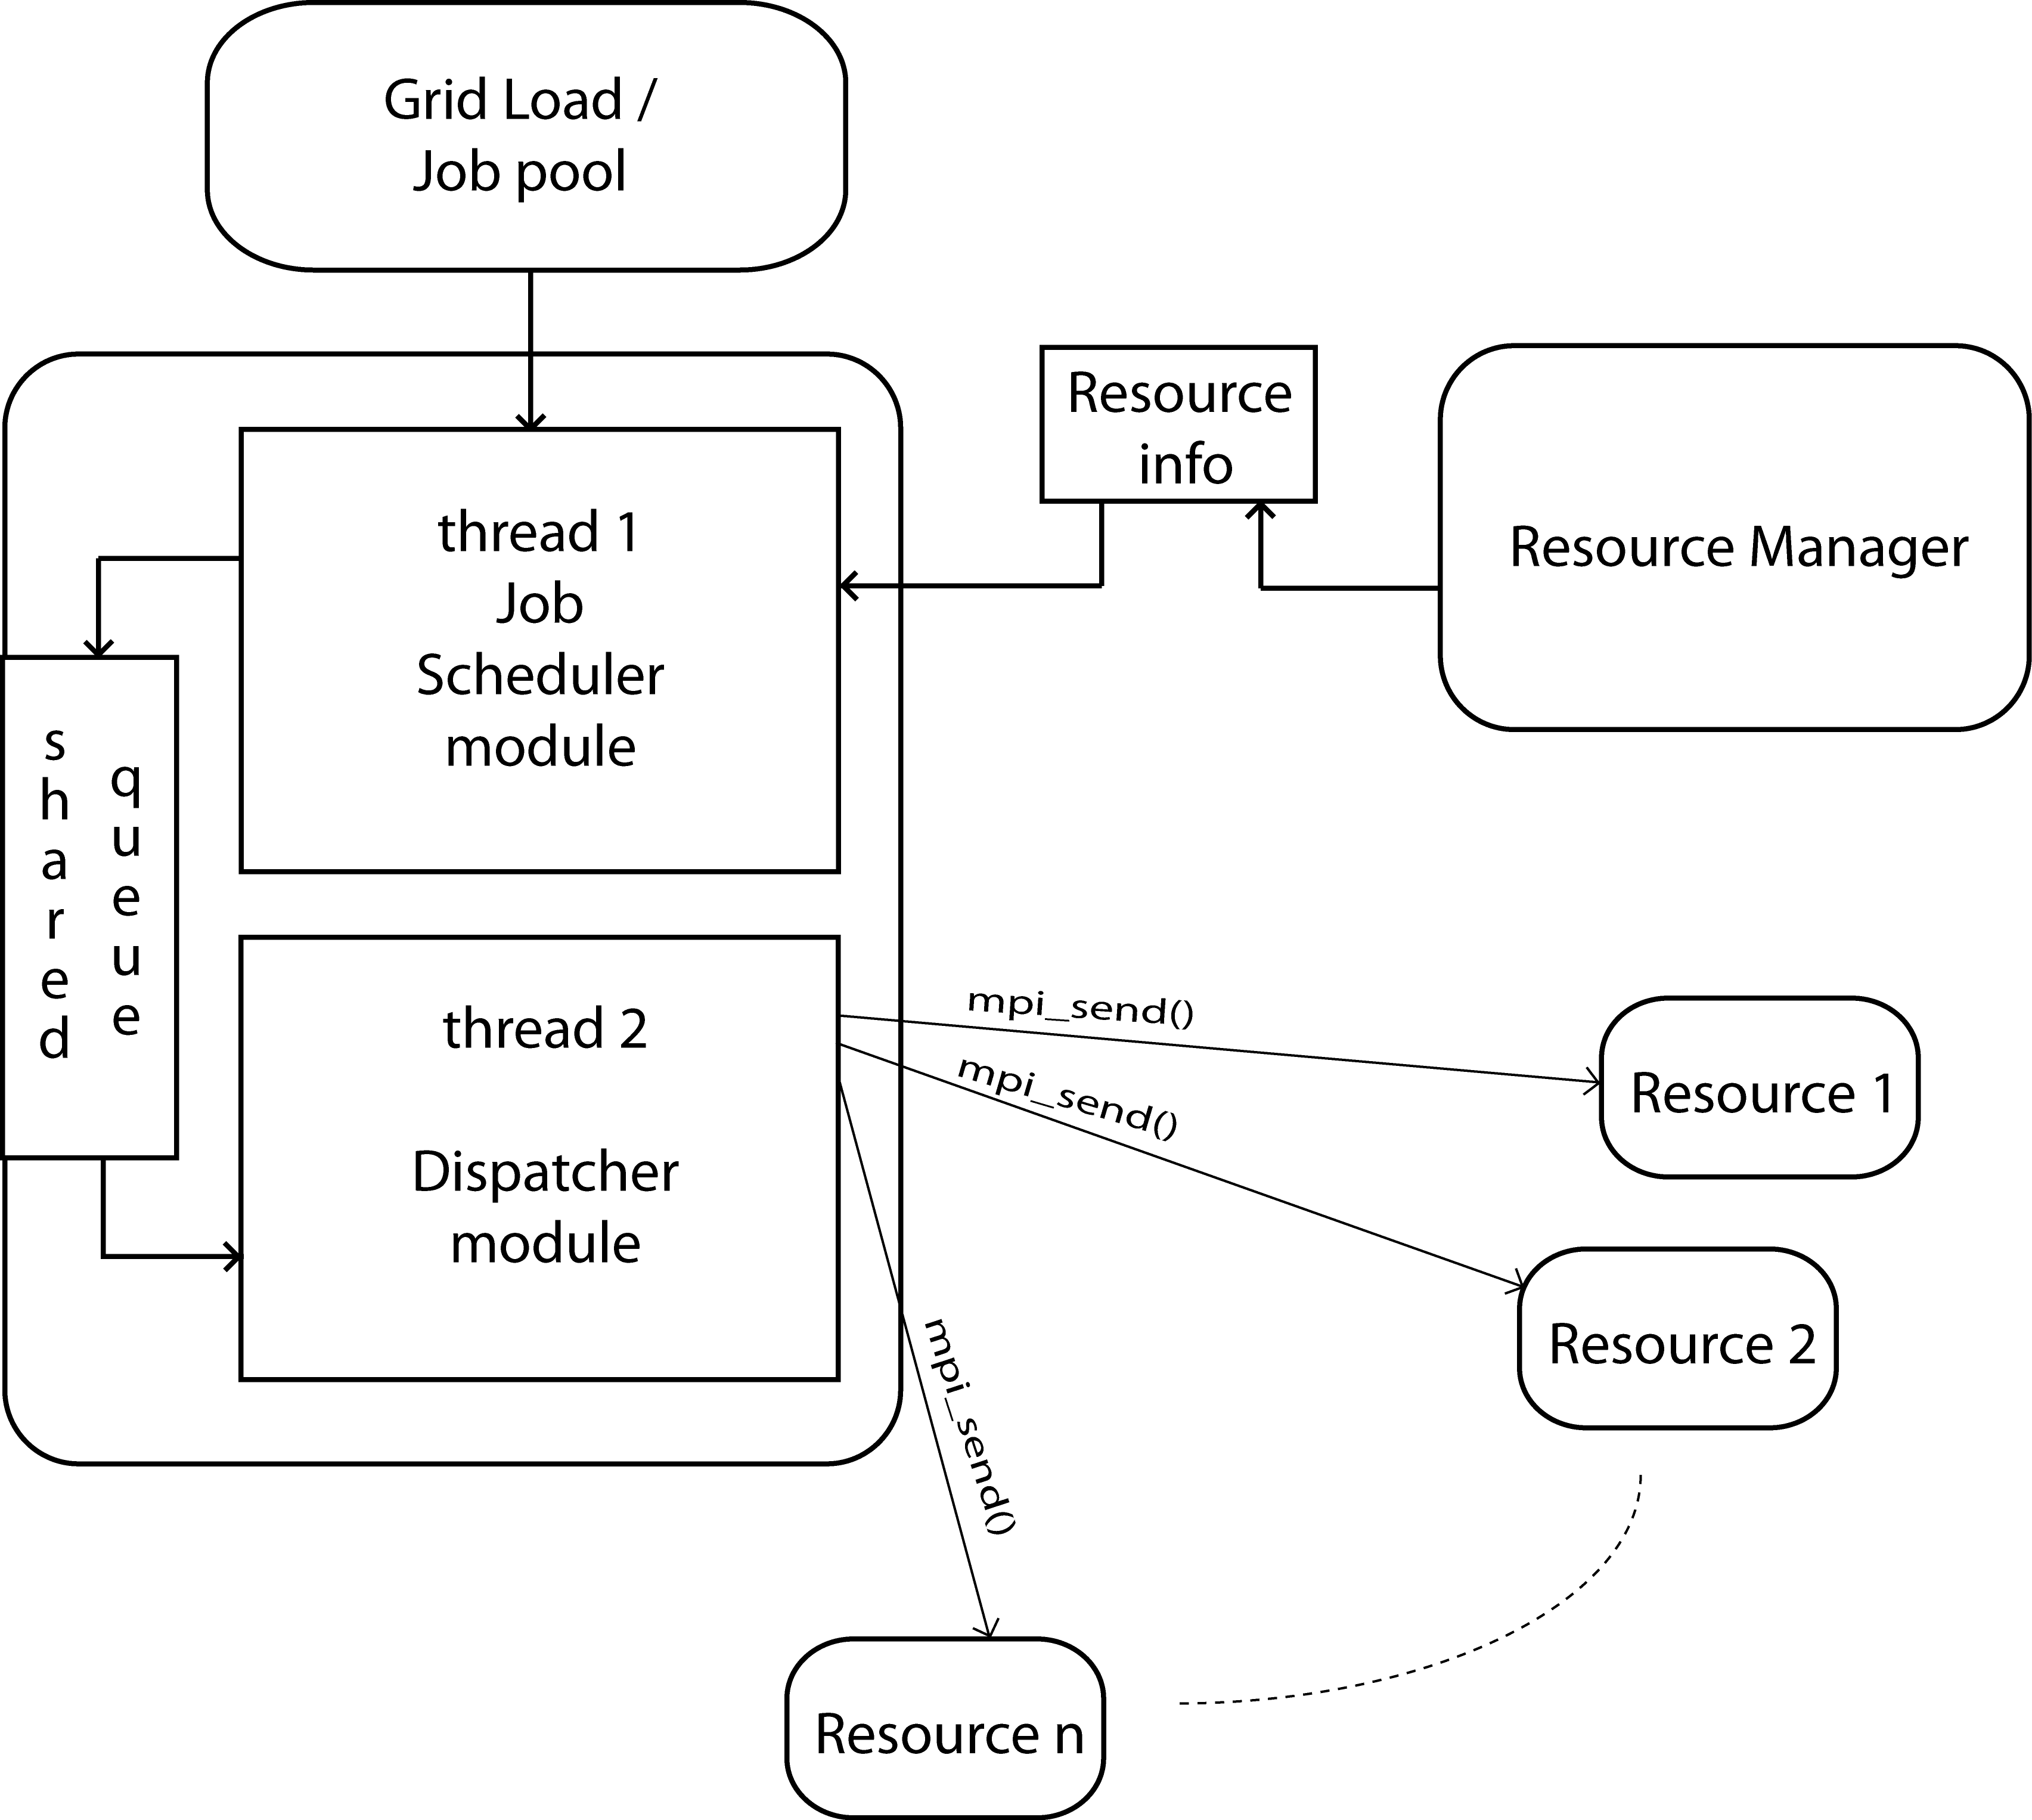
\includegraphics[width=1.0\columnwidth]{implement}
    \caption{Implemented System model}
	\label{fig:Systemmodel}
\end{figure}
\begin{itemize}
 \item Preprocessing of fine-grained jobs for reducing computing complexity of job scheduler.
 \item Flexibility of choosing best scheduling strategy from first pareto front. First pareto front represents non-dominating sets of strategies based on objective parameters.
 \item Normalized weighted sum approach, where weights can be changed dynamically assigned based on the change in grid behaviour.
 \item Configuring resources on the fly. Adding, modifying and deleting resources via resource manager.
 \item Real time job scheduler.
\end{itemize}
\section{System model}
Here we discuss detailed architecture of the implemented system. We have used posix thread to share the scheduling or mapping queues with the dispatcher. The Multi-objective Job Scheduler module run on one thread and dispatcher on another. The scheduler act as a producer and the dispatcher as a consumer. To simulate the grid environment the dispatcher sends job details through MPI to its mapped resource. The resources waiting for the messages on receiving job, run dummy jobs with the parameters passed on to it. Figure~\ref{fig:Systemmodel} is the schematic representation of the implemented system.\\
Dispatcher and scheduler maintains separate queues for separate resources. When  a resource goes down, jobs of that queue is rescheduled on available resources.
\subsection{Job queue}
It have been considered that a job requires a single core of processor for execution. Table~\ref{jobmodel} represents a segment of job queue.
Each grid job has following properties:
\begin{itemize}
 \item $JOB\_ID$ is an unique identifier for a job.
 \item Grid jobs are either CPU intensive or I/O intensive represented as $JOB\_TYPE$ 0/1 respectively.
 \item $PRED\_ID$ is the predecessor job on which the job is dependent. $-1$ represent no dependencies on other job.
 \item $JOB\_SIZE$ of CPU intensive jobs are either represented in MI (Million Instruction). % or Execution time scaled with a fixed MIPS.
 \item $JOB\_SIZE$ of I/O intensive jobs are either represented in MB (Mega Bytes). % or Transfer time scaled with a fixed MBPS.
 \item $TIME\_LIMIT$ is a constraint for job completion, exceeding time limit imposes penalty. Unit of $TIME\_LIMIT$ is seconds.
 \item $JOB\_COST$ is the expected cost to be incurred by the user based on the QoS agreement. Unit of $JOB\_COST$ is currency e.g. USD(\$).
\end{itemize}
\begin{table}[ht]
\caption{User job queue}
    \begin{tabular}{|c|r|c|c|c|c|}
    \hline \hline
    $JOB\_ID$ & $JOB\_SIZE$ & $TIME\_LIMIT$ & $JOB\_COST$ & $PRED\_ID$ & $JOB\_TYPE$ \\ 
     & in MI/MB & in seconds & in \$ &  &  \\ \hline
    $\vdots$ & $\vdots$ & $\vdots$   & $\vdots$ & $\vdots$	     & $\vdots$  \\
    42     & 24,000 MI  & 63.0  & 5.41 & 29                 & 0        \\
    43     & 130,000 MI  & 107.0 & 4.86 & -1                 & 0        \\
    44     & 10,500 MI  & 106.0 & 5.99 & 24                 & 0        \\ 
    47     & 530.0 MB  & 150.0 & 5.04 & 29   	       & 1	\\
    48     & 240,200 MI  & 133.0 & 5.40 & 31   	       & 0        \\
    $\vdots$ & $\vdots$ & $\vdots$   & $\vdots$ & $\vdots$	     & $\vdots$  \\ \hline
    \end{tabular}
\label{jobmodel}
\end{table}
\subsection{Resource model}
Resource manager configures each resource with the following properties. Table~\ref{resconf} shows configuration of some of the resources in grid.
\begin{itemize}
 \item $RESOURCE\_ID$ is an unique identifier for a resource.
 \item Resources are either computing resource or storage resource represented as $RES\_TYPE$ 0/1 respectively.
 \item Computational resource processing capability is measured in MIPS (Million Instruction per second) or IPS(Instruction Per second) per core, and for storage resources it is measured in MB/s. We denote it as $RES\_CAP$ \cite{wiki_CPU}.
 \item Another resource parameter is power dissipation/consumption figure in watts. $RES\_ENERGY$ is also represented in a normalized form \cite{wiki_wattage}.
\end{itemize}
\begin{framed}
{\small
	     Resource power dissipation figure is measured in Watts. Resource with maximum power dissipation figure is found and scaled to 1.0. Similarly other resources power dissipation figures are scaled with maximum power dissipation figure. For example Intel Core i7 920 (Quad core) consumes 130 Watts and Intel Core 2  X6800 (Dual core) consumes 75 Watts, 130 Watts is normalized to 1.0 and 75 Watts to 0.577 \cite{wiki_wattage}.
}
\end{framed}
\begin{itemize}
 \item $RES\_COST$ is the cost of the resource per second.
\end{itemize}
Resources manager module updates available resources information in a file which is being read  by Job scheduler module before each run.
\begin{table}[ht]
\caption{Resource configuration}
    \begin{tabular}{|c|r|c|c|r|}
    \hline \hline
    $RESOURCE\_ID$ & $RES\_COST$ & $RES\_TYPE$ & $RES\_ENERGY$  & $RES\_CAP$ \\ 
     & in \$ &  & \emph{normalized}  & {\small in MIPS/MBPS} \\ \hline \hline
    $\vdots$ & $\vdots$ & $\vdots$   & $\vdots$ & $\vdots$  \\
    4 & 0.13 & 0 & 0.943 & 9,726 MIPS   \\
    5 & 0.14 & 0 & 1.000 & 29,621 MIPS   \\
    6 & 0.13 & 0 & 0.577 & 13,539 MIPS \\
    7 & 0.11 & 1 & 0.894 & 30.0 MBPS     \\
    $\vdots$ & $\vdots$ & $\vdots$   & $\vdots$ & $\vdots$  \\ \hline
    \end{tabular}
\label{resconf}
\end{table}

\subsection{Output of scheduler}
The scheduler yields mapping of jobs and resources with start time and expected execution time of each job. Each resource has its own queue. A queue of jobs mapped to resource id 1 is shown in Table~\ref{tab:out}
\begin{table}[ht]
\caption{Mapping queue for RESOURCE\_ID 1}
 \centering
    \begin{tabular}{|c|c|r|r|}
    \hline \hline
    $JOB\_ID$ & $RES\_ID$ & $START\_TIME$ & $EXEC\_TIME$ \\ 
     &  & in seconds & in seconds \\ \hline \hline
    $\vdots$ & $\vdots$ & $\vdots$   & $\vdots$ \\ 
    95255	& 1	& 952.42	& 138.30 \\ 	
    95259	& 1	& 1090.73	& 78.58 \\ 
    95205	& 1	& 1169.31	& 37.71 \\ 
    95306	& 1	& 1207.03	& 62.86 \\ 
    95301	& 1	& 1269.90	& 59.72 \\ 
    95337	& 1	& 1329.62	& 194.88 \\
    $\vdots$ & $\vdots$ & $\vdots$   & $\vdots$ \\ \hline \hline
    \end{tabular}
\label{tab:out}
\end{table}

\subsection{Randomize function}
In any stochastic algorithm randomize function plays an important role. A very fast random number generator Mersenne Twister of period $2^{19937}-1$ is used in different parts of the code and has a better equidistibution property. It generates integer in the range $0$ to $2^{32}-1$ and real number range $[0,1)$ with a precision of $2^{32}$ \cite{saito2007application}.

\section{Data Sets}
\label{datasets}
Standard grid workload from Grid Workload Archive have been used in this experiments \cite{gridload}. The traces and logs of different grid environments are given in standard gwf format. Gridloads are processed to add a few more parameters like cost of jobs, jobs time limit for completion, predecessor dependencies among jobs and type of jobs. \\
SHARCNET \& DAS-2 are the two traces that have been processed. Traces shows that execution time of jobs ranges from 1 to 20000 time units in DAS-2, and 1 to 100000 time units in SHARCNET. This shows job characteristic varies widely making scheduler task difficult.\\
For analyzing the performance based on various parameters following workloads have been created given in Table ~\ref{tab:gridlet}.

\begin{table}[ht]
\caption{Gridlet configuration}
\centering
    \begin{tabular}{|c|c|c|c|}
    \hline \hline
    Workload\_id & Trace        & Precedence constraint & Resource constraint \\ \hline
    1 	         & DAS-2    & \xmark                 & \xmark   \\
    2 	         & SHARCNET & \xmark                 & \xmark   \\
    3 	         & DAS-2    & \xmark                 & \cmark   \\
    4 	         & SHARCNET & \xmark                 & \cmark   \\
    5	         & DAS-2    & \cmark                 & \xmark   \\
    6	         & SHARCNET & \cmark                 & \xmark   \\
    7	         & DAS-2    & \cmark                 & \cmark   \\
    8 	         & SHARCNET & \cmark                 & \cmark   \\ \hline \hline
    \end{tabular}
\label{tab:gridlet}
\end{table}
\begin{framed}
 Workloads are created on the basis of imposing constraints on traces. Job precedence rule is referred to as precedence constraint and constraint of executing jobs on particular type of resource is referred to as resource constraint. Predecessor jobs have been created with the statistics given in table~\ref{pcons}
\end{framed}
\begin{table}[h]
\caption{Precedence Constraints}
\centering
    \begin{tabular}{|c|c|}
    \hline \hline
    Percentage of Jobs & 50\%  \\ \hline \hline
    Range & [JOB\_ID -100 , JOB\_ID -1] \\ \hline
    Mean  & [JOB\_ID -50] \\ \hline
    Variance & 20 \\ \hline \hline
    \end{tabular}
\label{pcons}
\end{table}

\section{Results}
In order to evaluate the performance of our scheduler we have performed set of experiments on the workloads mentioned in section~\ref{datasets}. The scheduler can schedule 200 jobs in 21 seconds. For more optimized results chromosome population and iteration in our algorithm can be increased. 
\subsection{Experiment on independent jobs}
Experiment results given in Figure ~\ref{fig:10res},~\ref{fig:15res},~\ref{fig:20res},~\ref{fig:25res} on workload 1 and 2 shows minimization of makespan and proper utilization of resources on independent jobs. 
Result shows that irrespective of the large variation of granularity in grid jobs we have achieved 99\%+ utilization performance in almost every resource. Result shows the scalability of our scheduler, we have tested the scheduler with 5000, 10000, 15000, 20000, 25000 jobs; and on 10, 15, 20, 25 resources. This shows that scheduler can process large amount of gridlets and resources without compensating on the Makespan and utilization of resources. The scheduler have yield near optimal mapping strategy optimizing on the time limit limit penalty and cost penalty referred in section ~\ref{formulation}.
\begin{figure}[!ht]
    \centering
    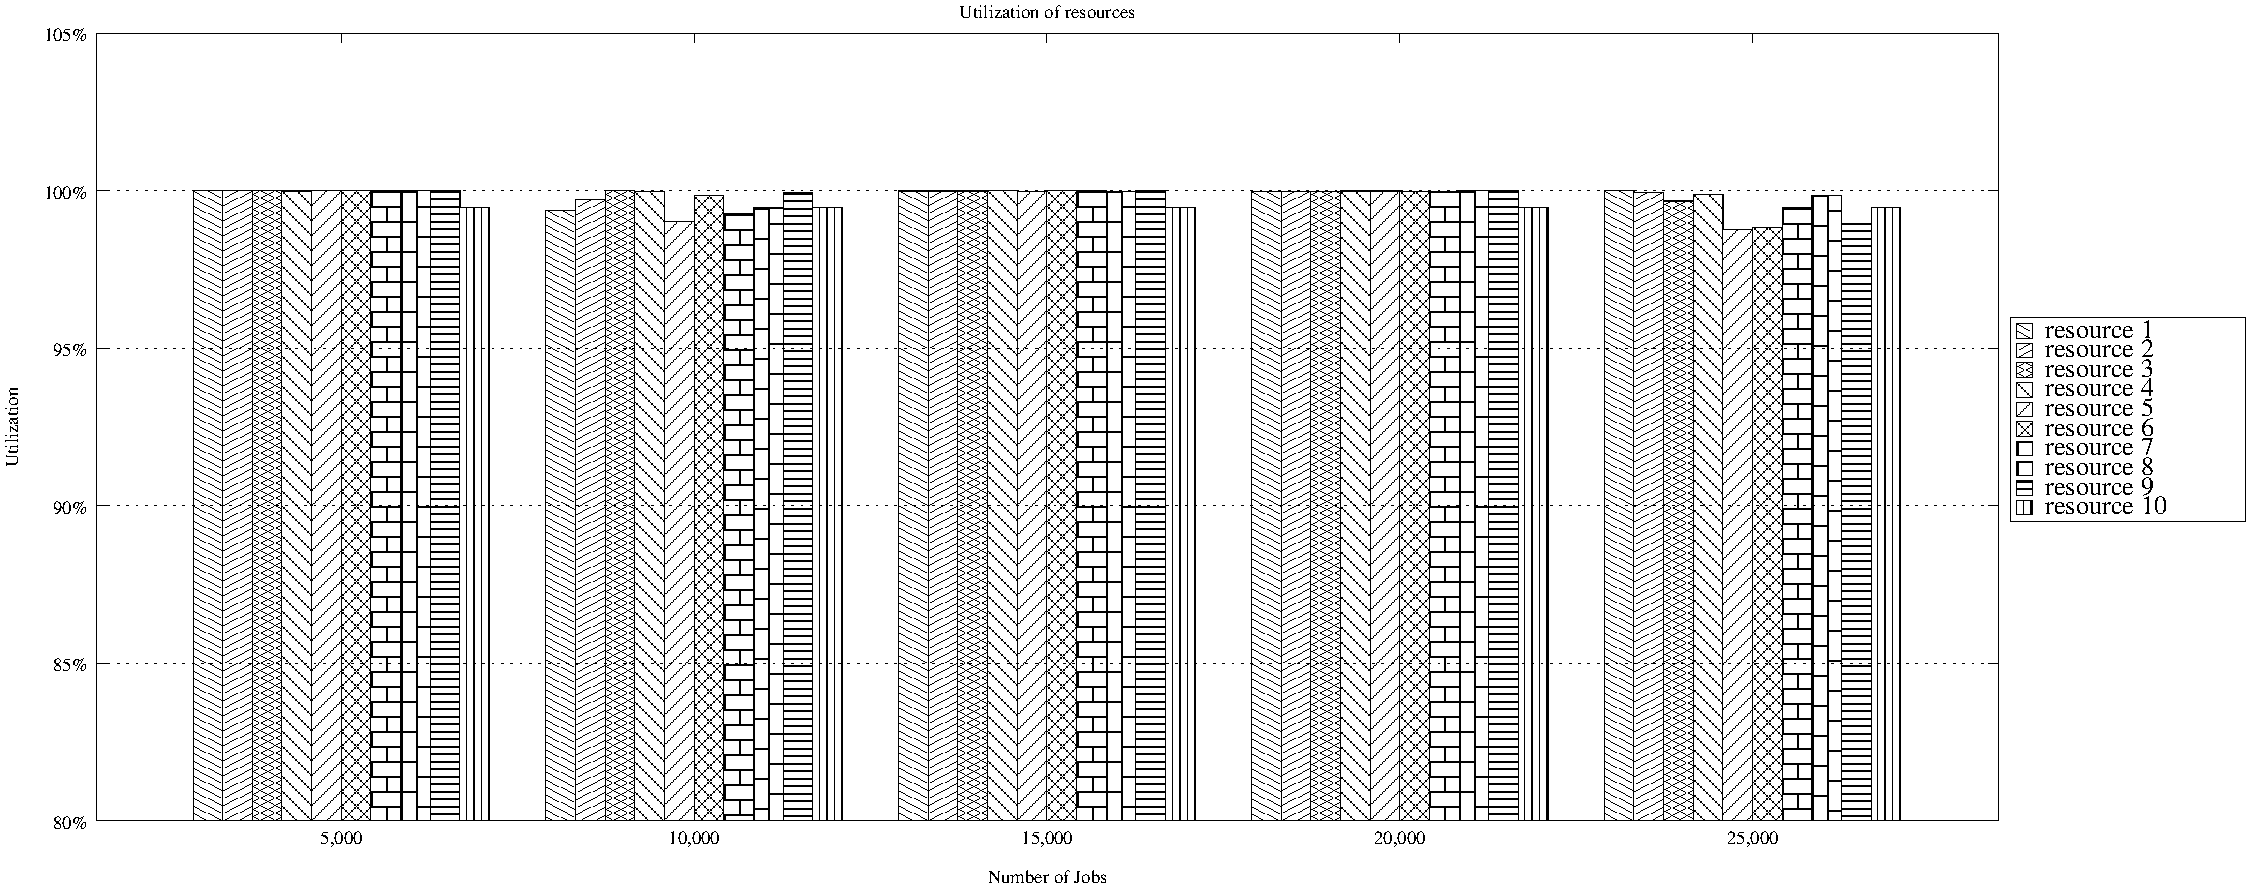
\includegraphics[width=1.5\textwidth,keepaspectratio,angle=90]{10res_SHARCNET}
    \caption{Evaluation of makespan and utilization on 10 resources on workload 2}
    \label{fig:10res}
\end{figure}
\begin{figure}[!ht]
    \centering
%    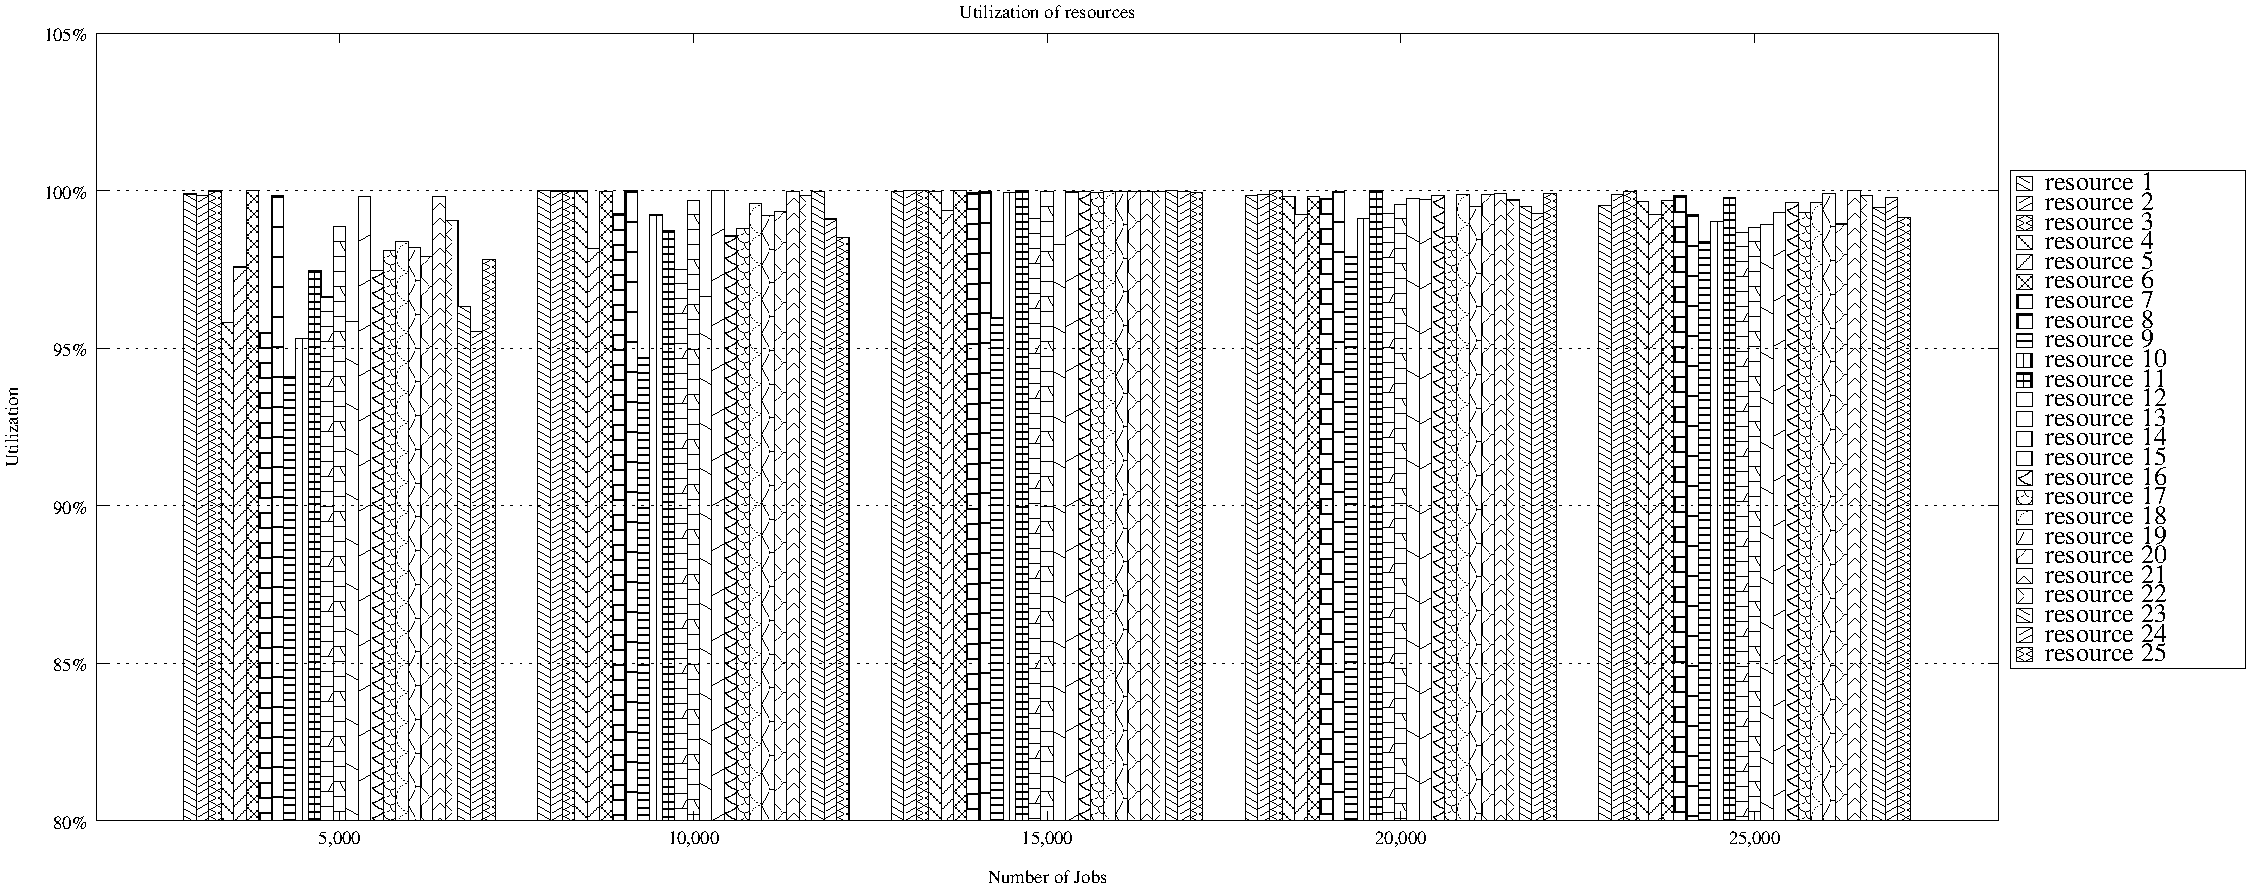
\includegraphics[width=1.1\columnwidth]{25res_SHARCNET}
%    \subfigure[\small ]{
    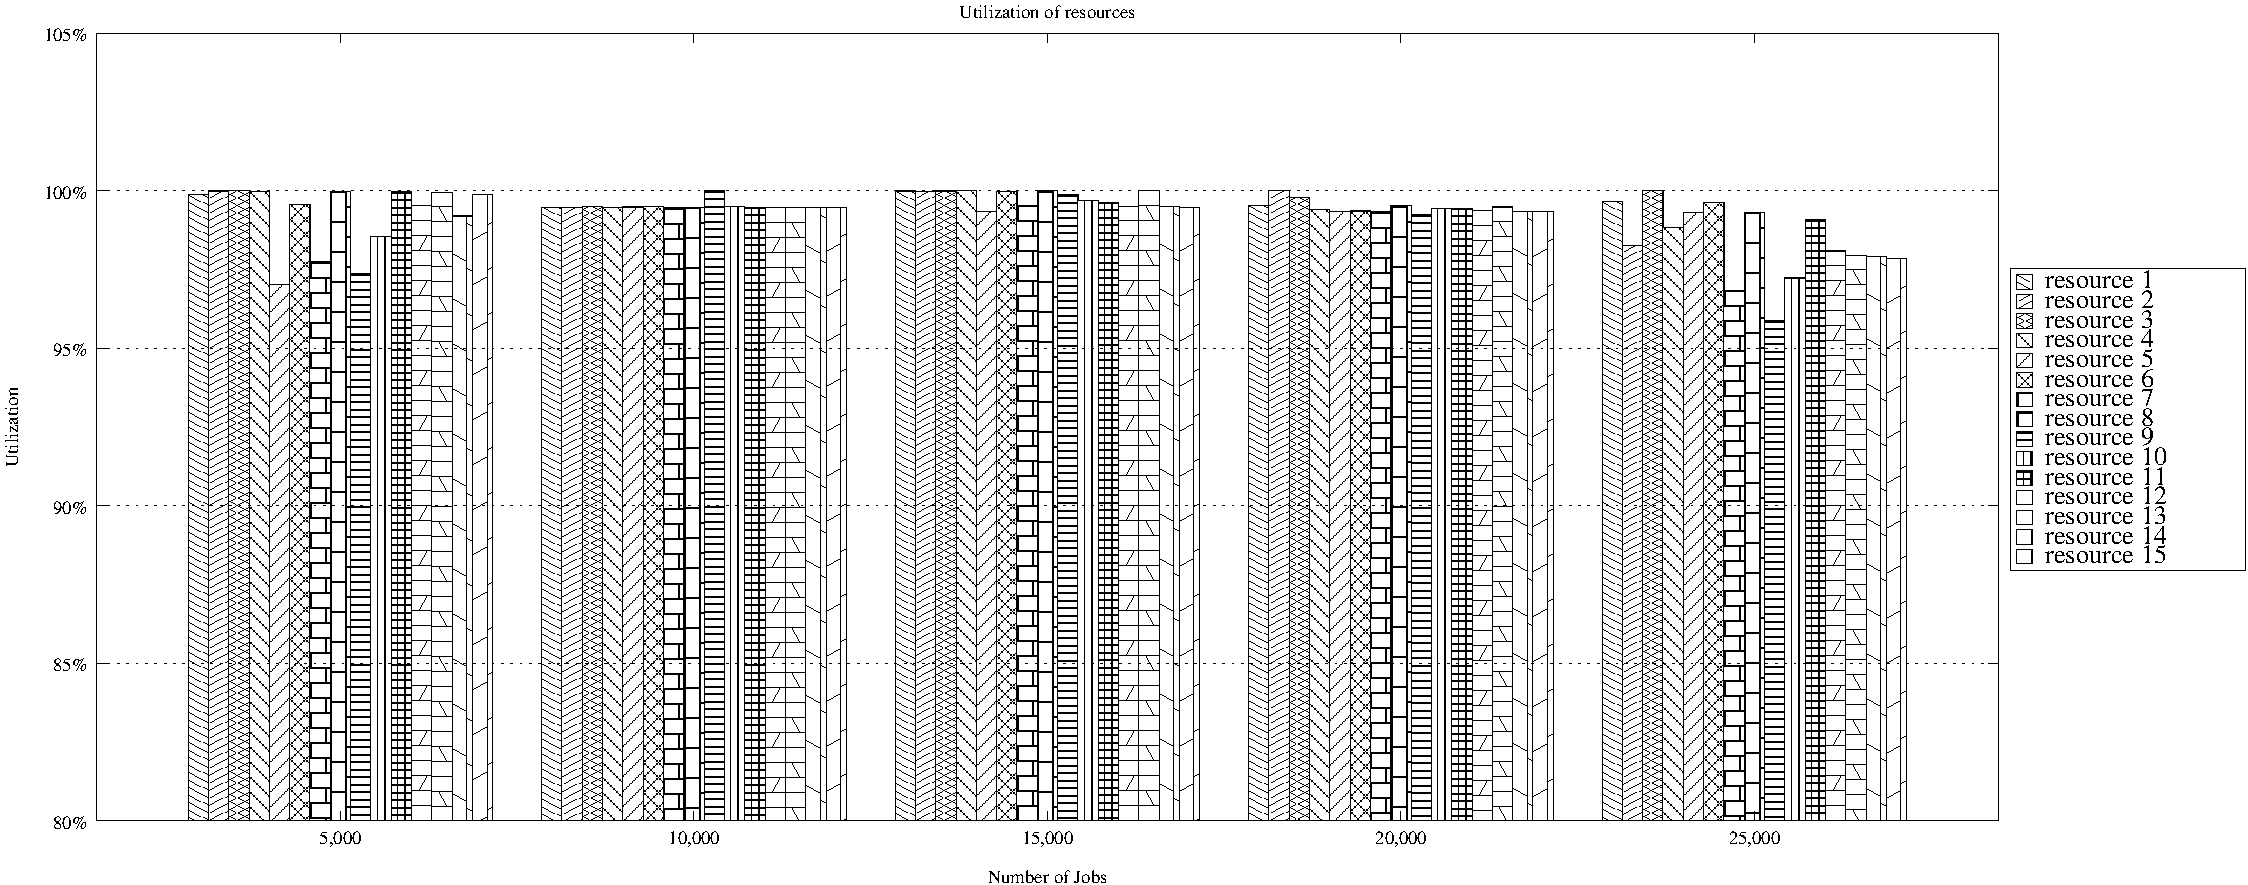
\includegraphics[width=1.5\textwidth,keepaspectratio,angle=90]{15res_SHARCNET}
    \caption{Evaluation of makespan and utilization on 15 resources on workload 1}
    \label{fig:15res}
\end{figure}
\begin{figure}[!ht]
    \centering
    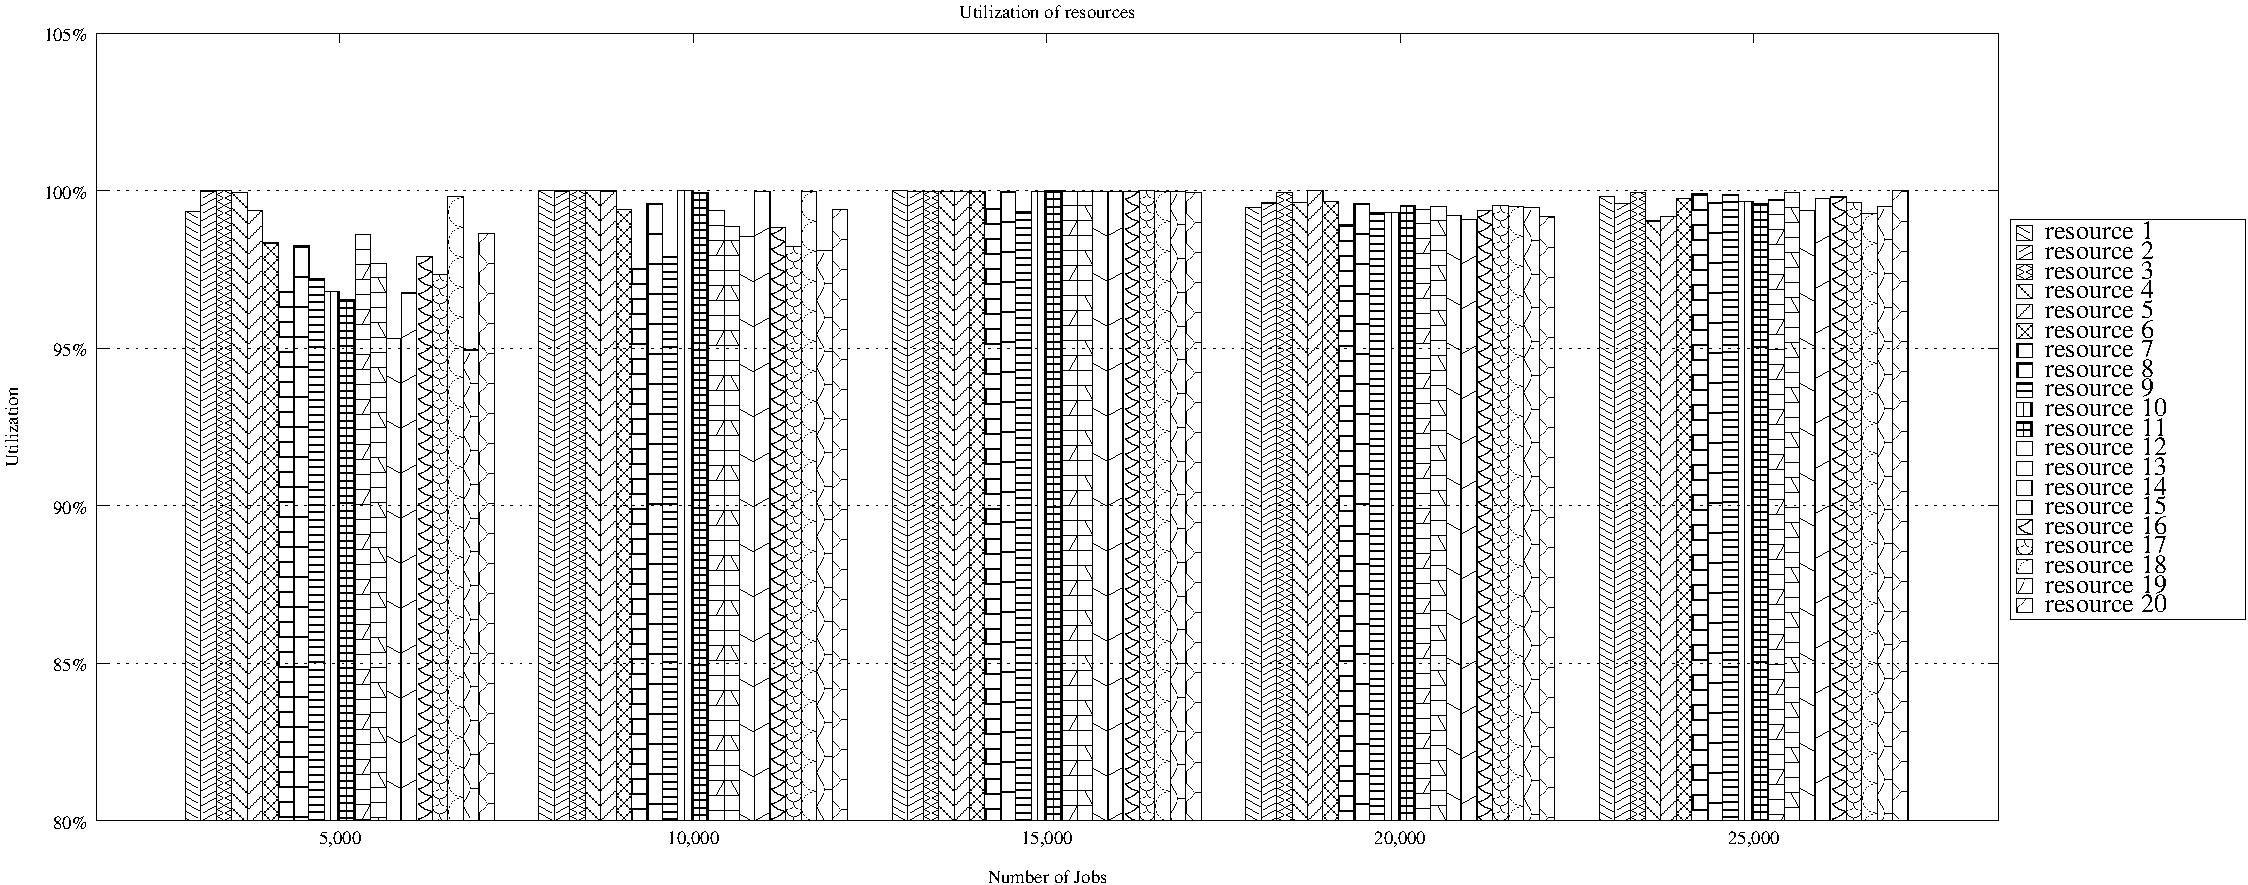
\includegraphics[width=1.5\textwidth,keepaspectratio,angle=90]{20res_SHARCNET}
    \caption{Evaluation of makespan and utilization on 20 resources on workload 1}
    \label{fig:20res}
\end{figure}
\begin{figure}[!ht]
     \centering
    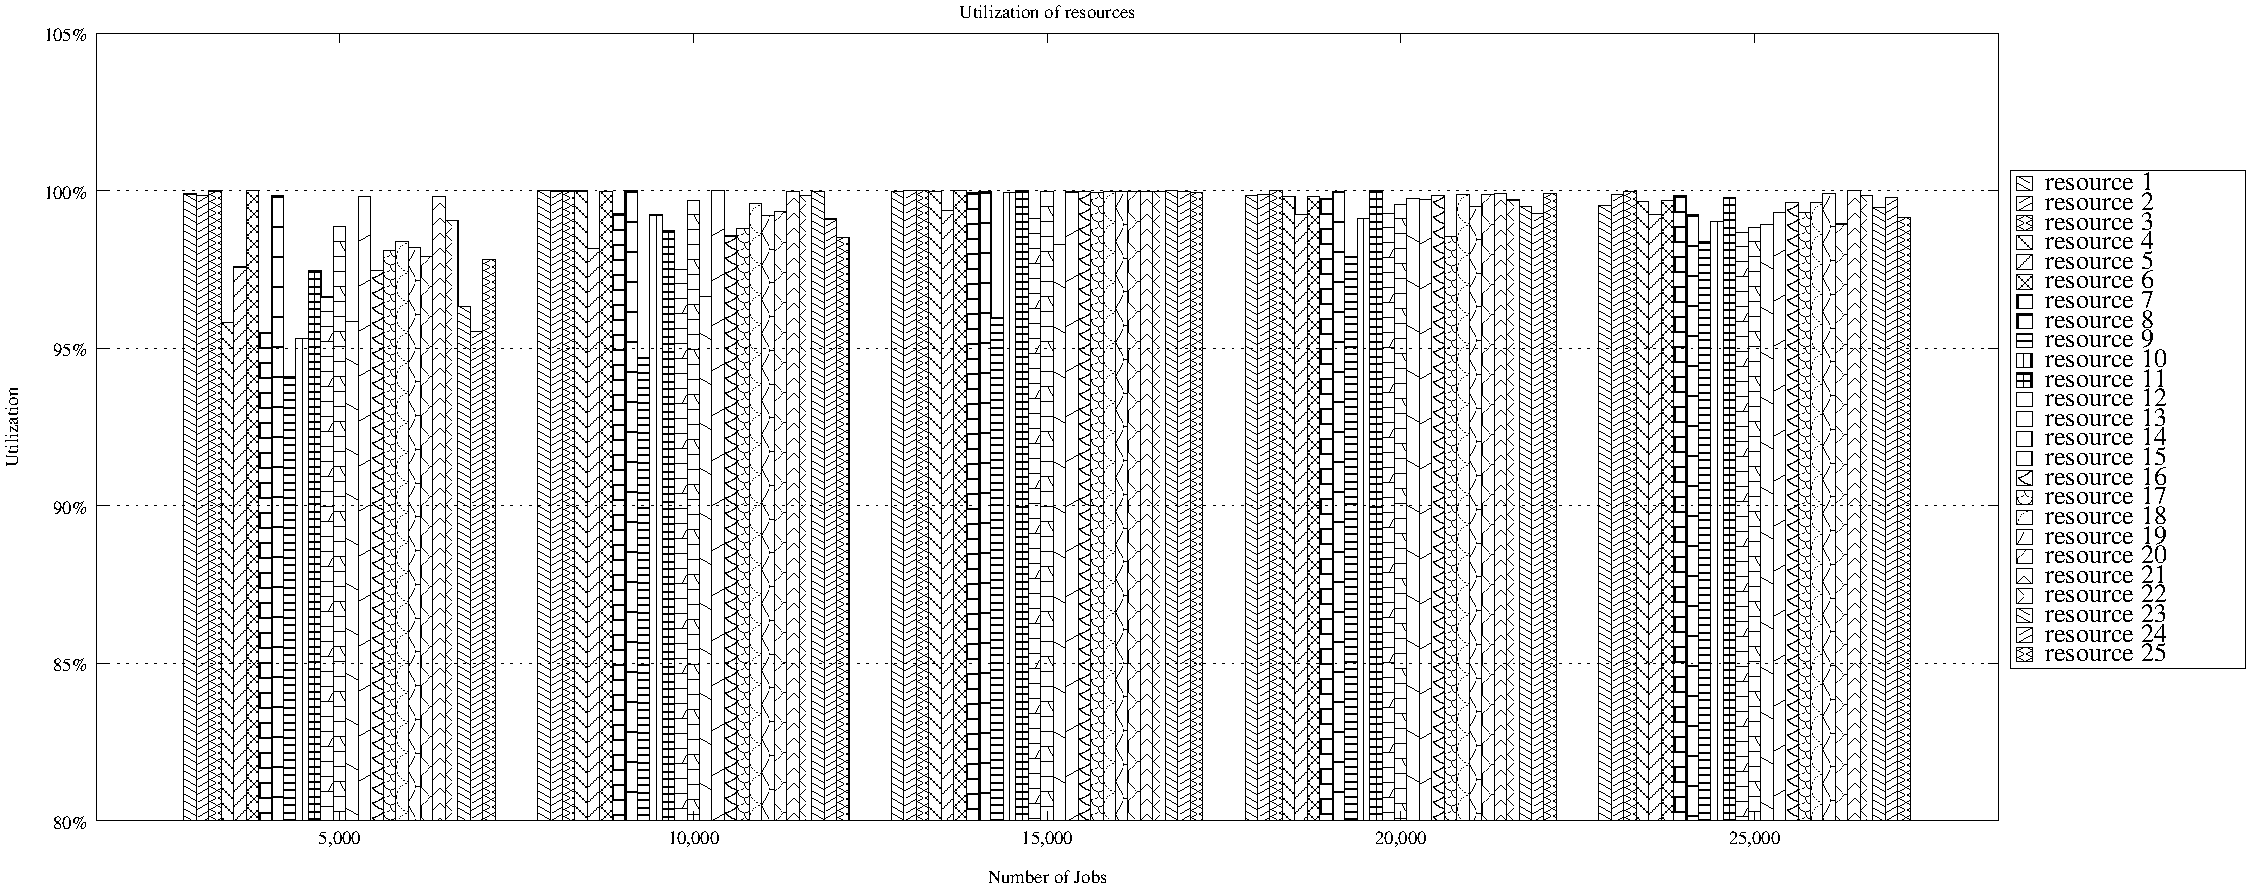
\includegraphics[width=1.5\textwidth,keepaspectratio,angle=90]{25res_SHARCNET}
    \caption{Evaluation of makespan and utilization on 25 resources on workload 2}
    \label{fig:25res}
\end{figure}
\subsection{Trade off between energy consumption and performance}
\label{case2}
\begin{figure}[h]
\centering
  \subfigure[\small Workload 2 (SHARCNET)]{
    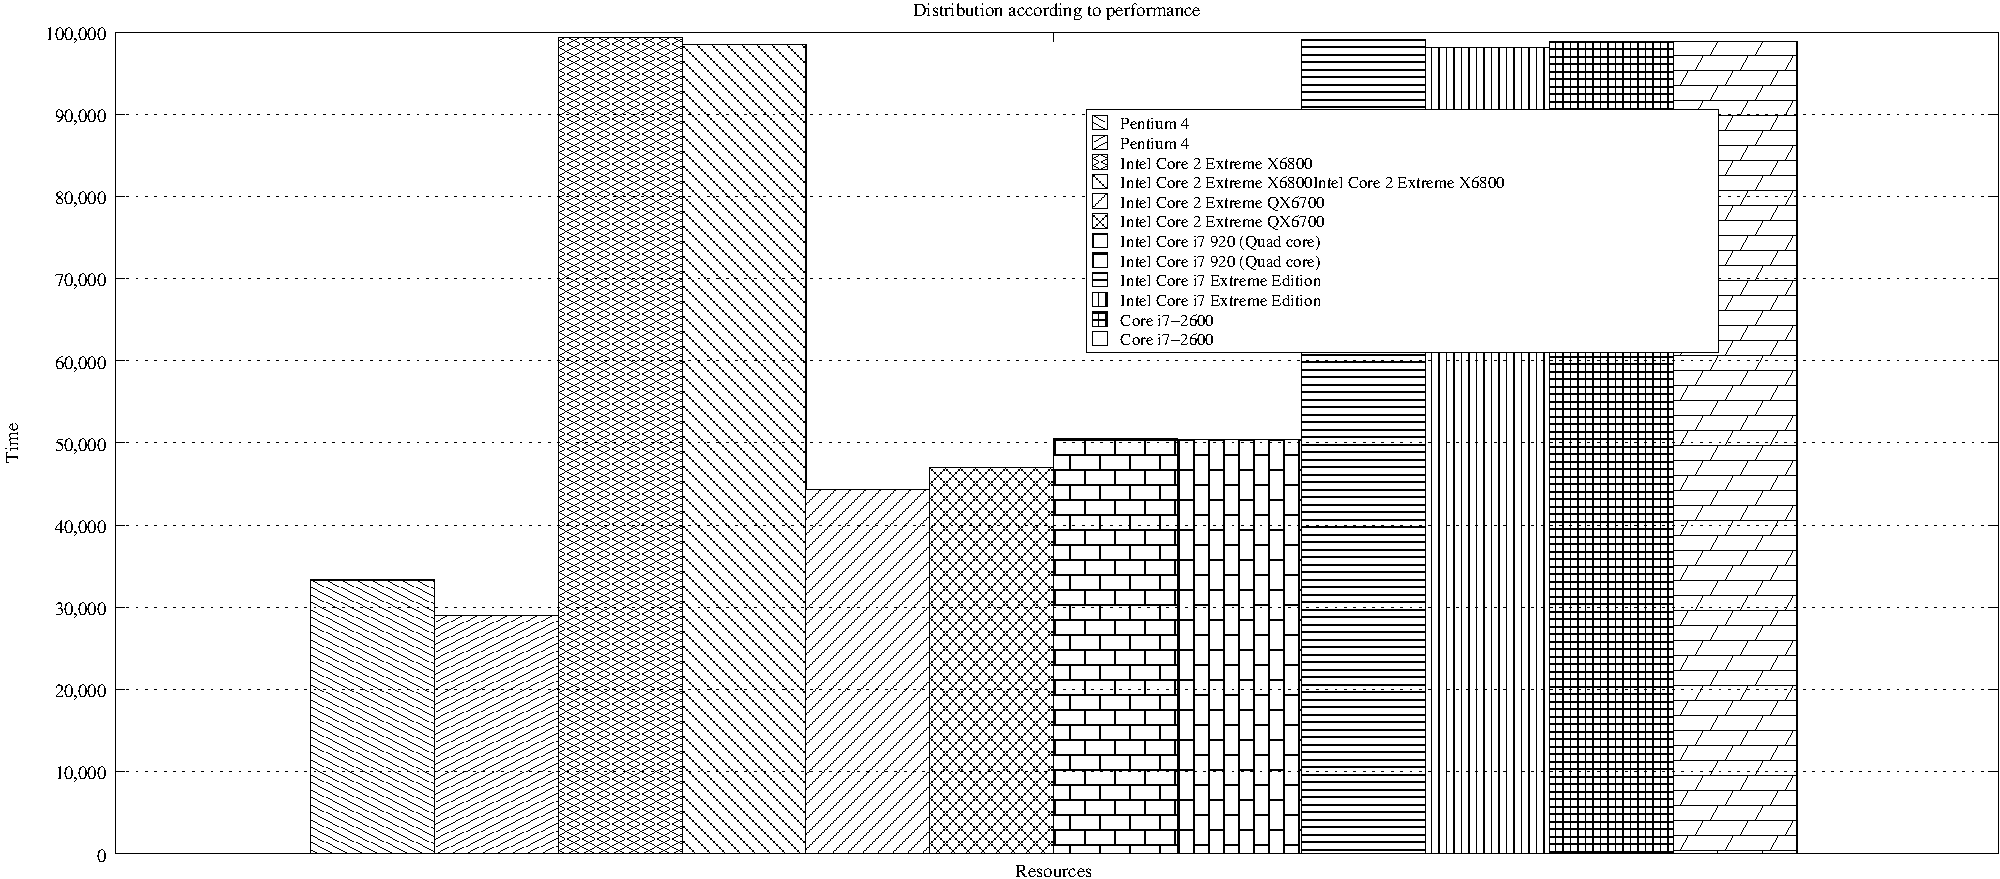
\includegraphics[width=1.0\columnwidth]{case2SHARCNET}
    \label{perform}
    }
    \subfigure[\small Workload 1 (DAS-2)]{
    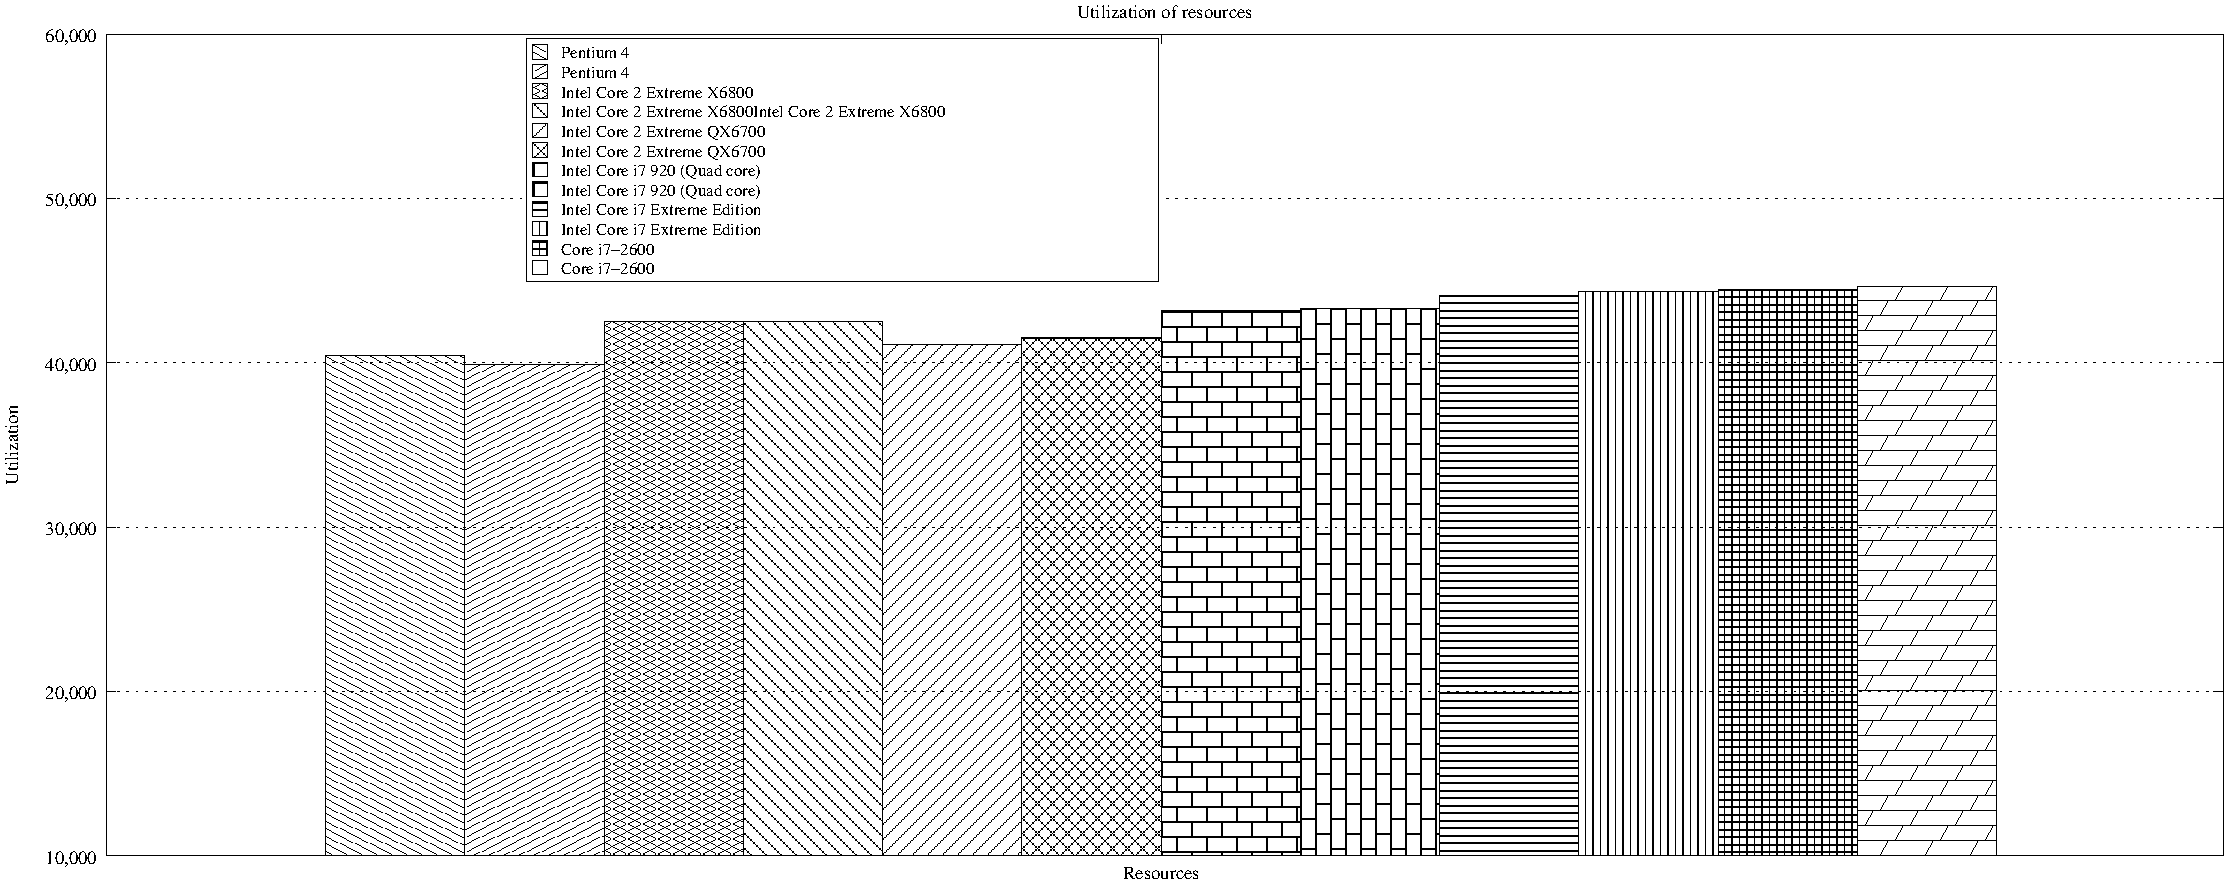
\includegraphics[width=1.0\columnwidth]{case2DAS}
    \label{perform1}
    }
\caption{ Evaluation of Ultilization on workload 1  and 2}
\end{figure}
Now energy parameter and performance parameter is considered while scheduling. It is worthy to note that if job is scheduled on high performance resource less time will be required for job completion and time limit constraint can be satisfied. Again, a job will try to be mapped on a  energy efficient resource minimizing overall power consumption. \\
Usually resources with high performing capability are less energy efficient. Jobs having large time limit can afford to be scheduled on low performance resource with low power consumption figures without being penalized for exceeding time limit. However high priority jobs needs high performance resource to process jobs within time limit.\\
The results given in Figure~\ref{perform} have been obtained by assigning equal weights on performance and energy efficiency objective on pareto front~\ref{pareto}.
Resource configuration for this experiment is given in Table~\ref{tab:res}.
\begin{table}[ht]
\caption{Resource configuration for experiment on workload 1 and 2 }
\centering
    \begin{tabular}{|l|l|c|c|c|}
    \hline \hline
    Machine & Frequency & Watts & MIPS/core & Resource\_id \\ \hline
Pentium 4 Extreme Edition 	&	3.2 GHz 	&	92.1	& 	9,726	 & 1,2 \\ \hline
Intel Core 2  X6800 (Dual core) 	&	2.93 GHz	&	75	&	13,539	& 3,4 \\ \hline
Intel Core 2  QX6700 (Quad core) 	&	2.66 GHz 	&	95	&	12,290 & 5,6	 \\ \hline
Intel Core i7 920 (Quad core) 	&	2.667 GHz 	&	130	&	20,575	 & 7,8 \\ \hline
Intel Core i7 3960X (Hex core) 	&	3.3 GHz	&	130	&	29,621	& 9,10  \\ \hline
Core i7-2600 	&	3.4 GHz	&	95	&	32,075	 & 11, 12 \\ \hline
\end{tabular}
\label{tab:res}
\end{table}
Experiment result for workload 2 is shown in Figure~\ref{perform}. Pentium 4 being poor in performance and energy dissipation factor as compared to other resources, have less uptime or running time. Now comparing resources Core 2 X6800 with Core 2 QX6700, they have almost same MIPS specification but Core 2 X6800 consumes less power. Figure~\ref{perform} shows that scheduler have allocated more jobs in Core 2 X6800 which is reasonable. Same logic can be applied for resources Core i7 920 and Core i73960X. They have same energy dissipation factor but Core i7 3960X performance is better. As a consequence scheduler have scheduled more jobs on Core i7 3960X. Best resource of the lot is Core i7-2600. The scheduler have uniformly distributed jobs among Core 2 X6800, Core i7 3960X and Core i7-2600 to have a minimum makespan.\\
Since workload 2 has large variation in the granularity of jobs the graph shows a worst case analysis in their utilization. In the best case scheduler will try to schedule jobs such that running time on each resource is same ~\ref{perform1}. \\
Figure~\ref{pareto} shows how our scheduler gives a better grip to the administrator to trade off between user objectives and grid administrator objectives. Each point on the space represents a scheduling strategy. In a 3D co-ordinate system we represents 3 objectives which are needed to be minimized namely (i) makespan (ii) Energy efficiency parameter, (iii) time targidity. Any point in the first pareto front can be chosen for scheduling strategy. This gives grid administrator wide range of choices and cope up with dynamic behaviour of grid.

\begin{figure}[h]
\centering
    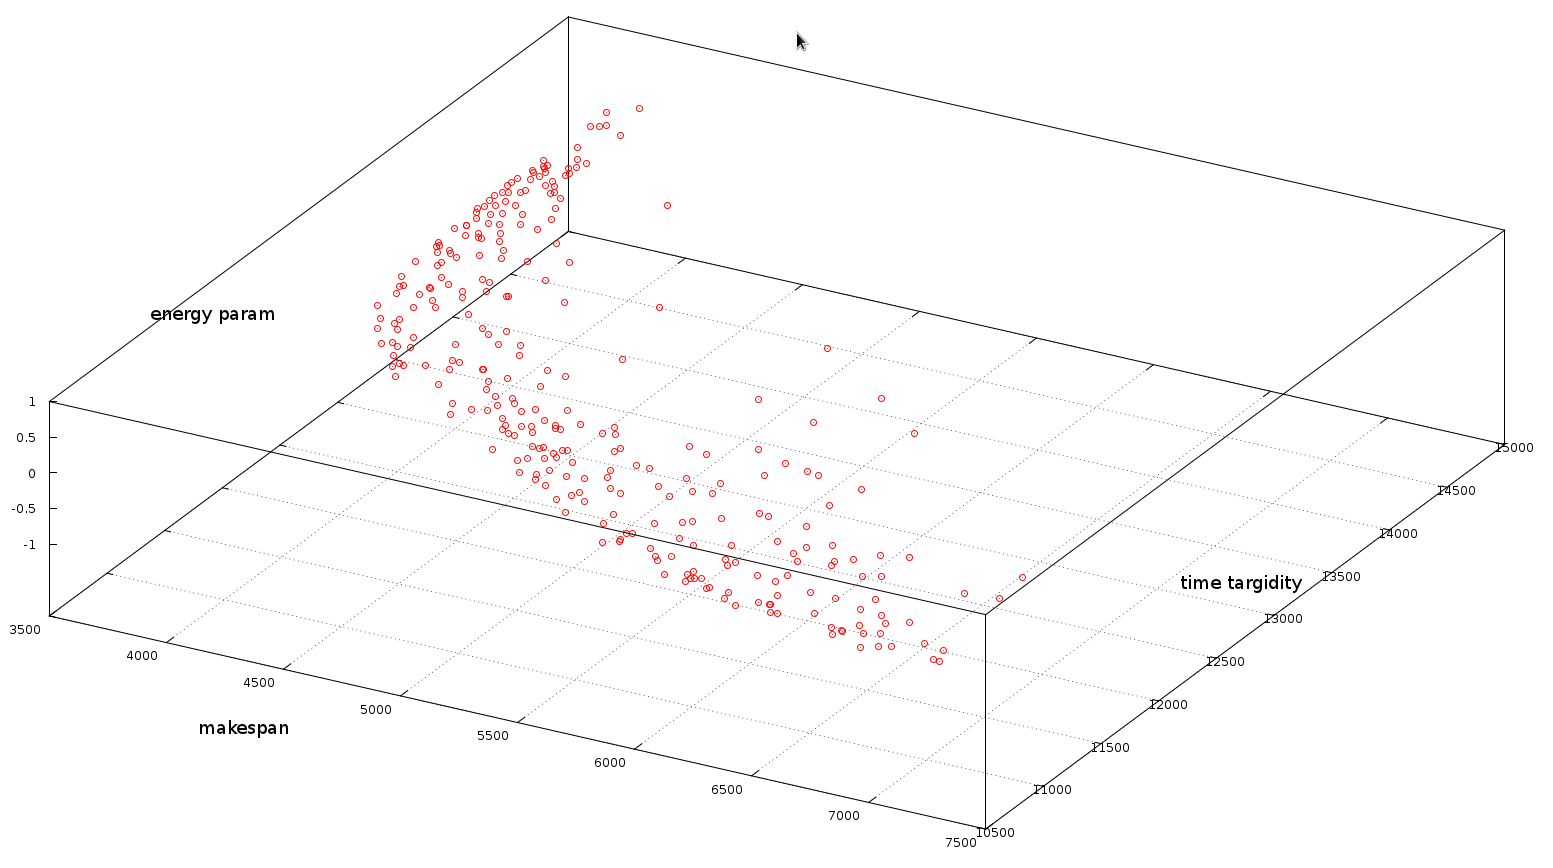
\includegraphics[width=1.0\columnwidth]{pareto2}
    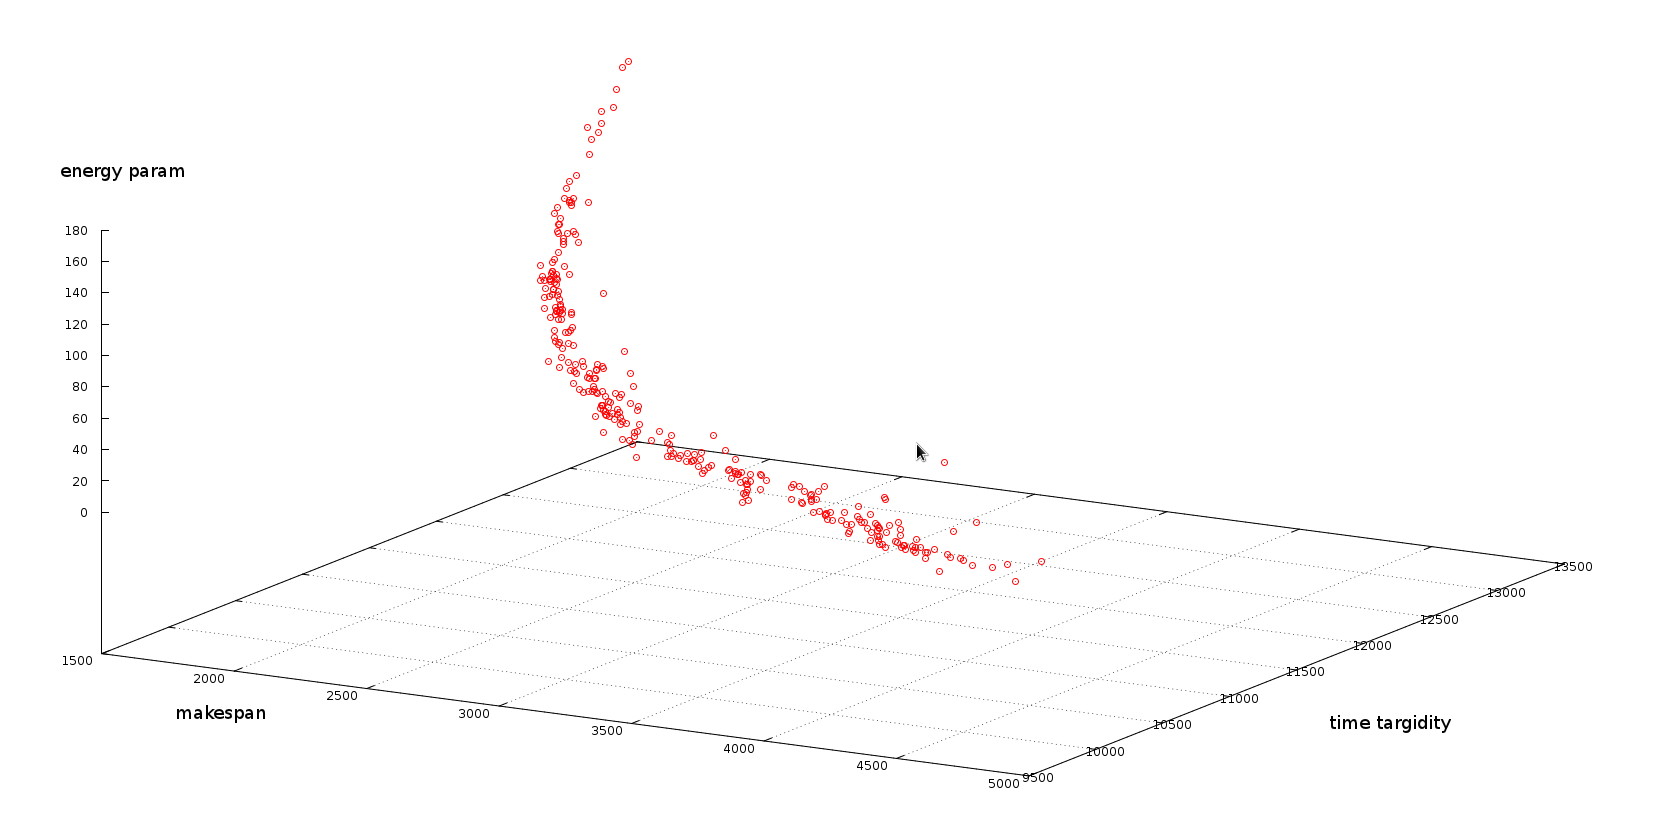
\includegraphics[width=1.0\columnwidth]{pareto}
    \caption{pareto front for makespan, time targidity and energy efficiency}
\label{pareto}
\end{figure}

\subsection{Experiment: Introducing job type constraint}
Now we introduce the job type constraint in our experimental analysis. Workload 3 and 4 referred in Table~\ref{datasets} have been used in this experiment. There are two type of jobs in the worload. On each workload we varied job percentage as 30\%-70\%, 50\%-50\%, 70\%-30\% to show the adaptiveness of our scheduler. 
A batch of 7000 jobs were taken which makes makespan of range $10^{7}$ to show the analysis in graph. Figure~\ref{jobtype1} shows uniform utilization among same type of resources inspite of the variance of job type percentage. One thing is further noticeable that analysis of section ~\ref{case2} still holds. Intel core i7 920 and Core i7-2600 performed equally well whereas Pentium 4 have disappointed again. \\
For choosing a scheduling strategy from first pareto front weighted sum technique on normalized objectives have been used. For the result shown in Figure~\ref{jobtype1} and ~\ref{jobtype2} equal weight was assigned on each objective.
\begin{figure}[h]
\centering
    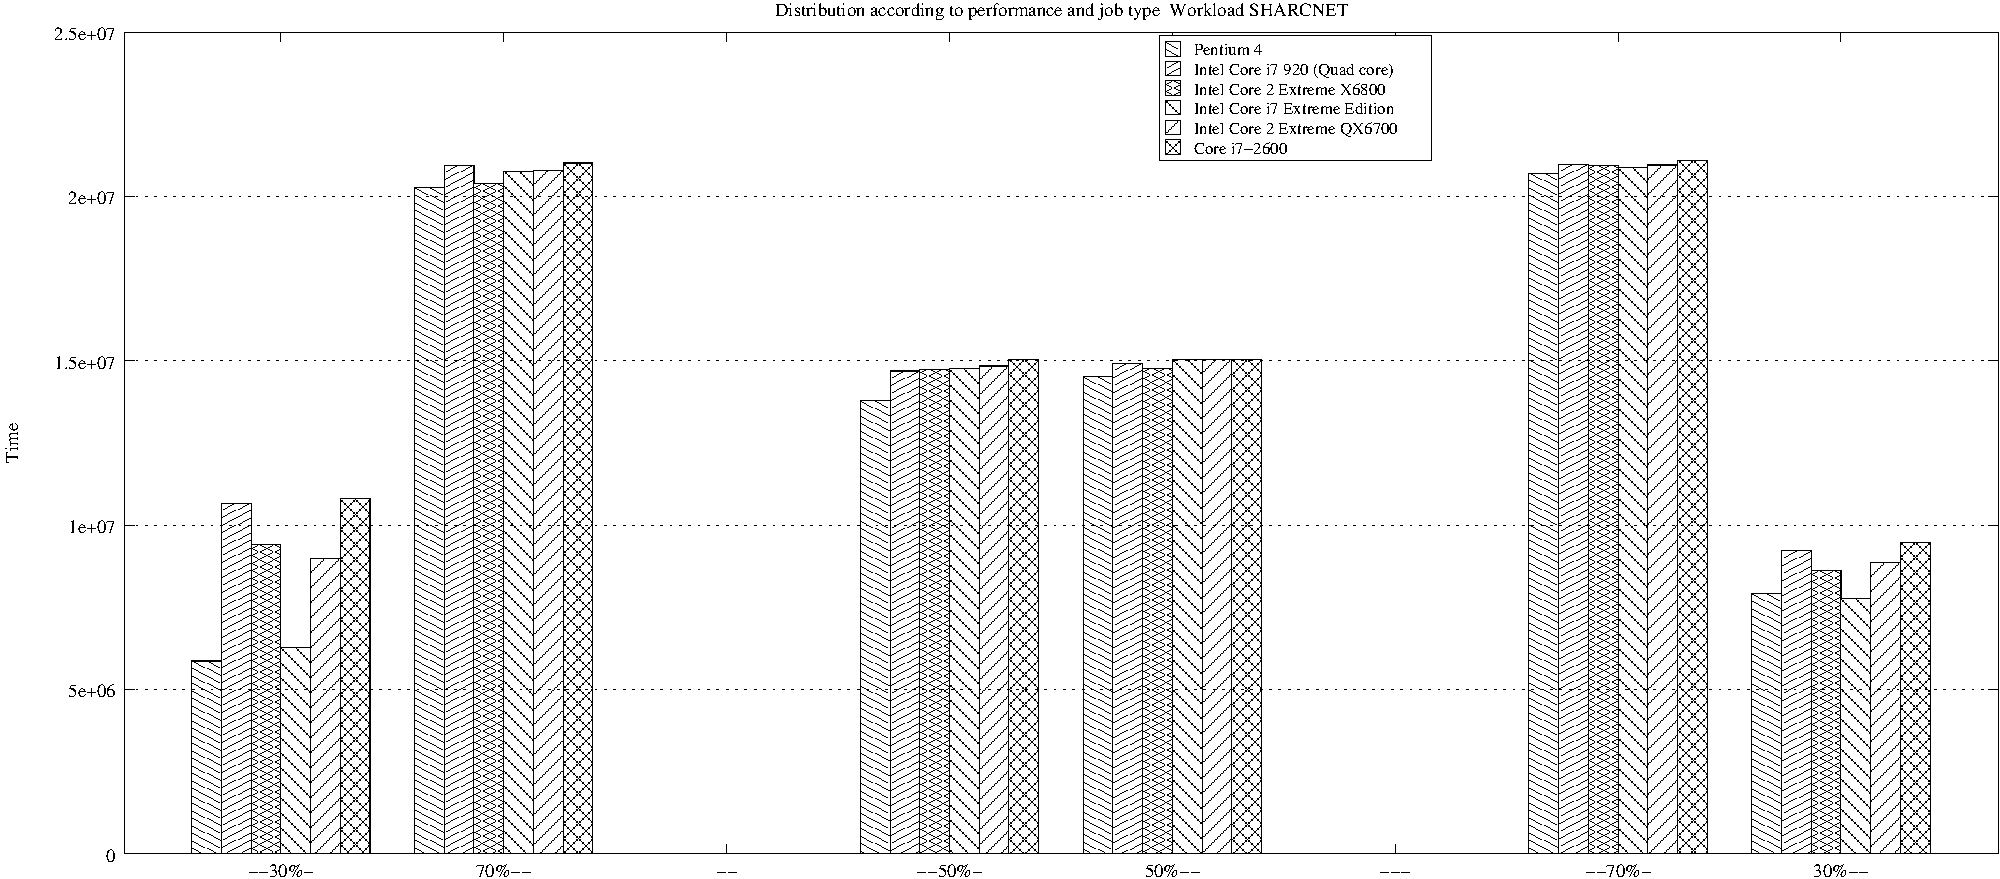
\includegraphics[width=1.0\columnwidth]{case3_SHARCNET}
    \caption{Performance under Job type constraint, SHARCNET Workload}
\label{jobtype1}
\end{figure}
\begin{figure}[h]
\centering
    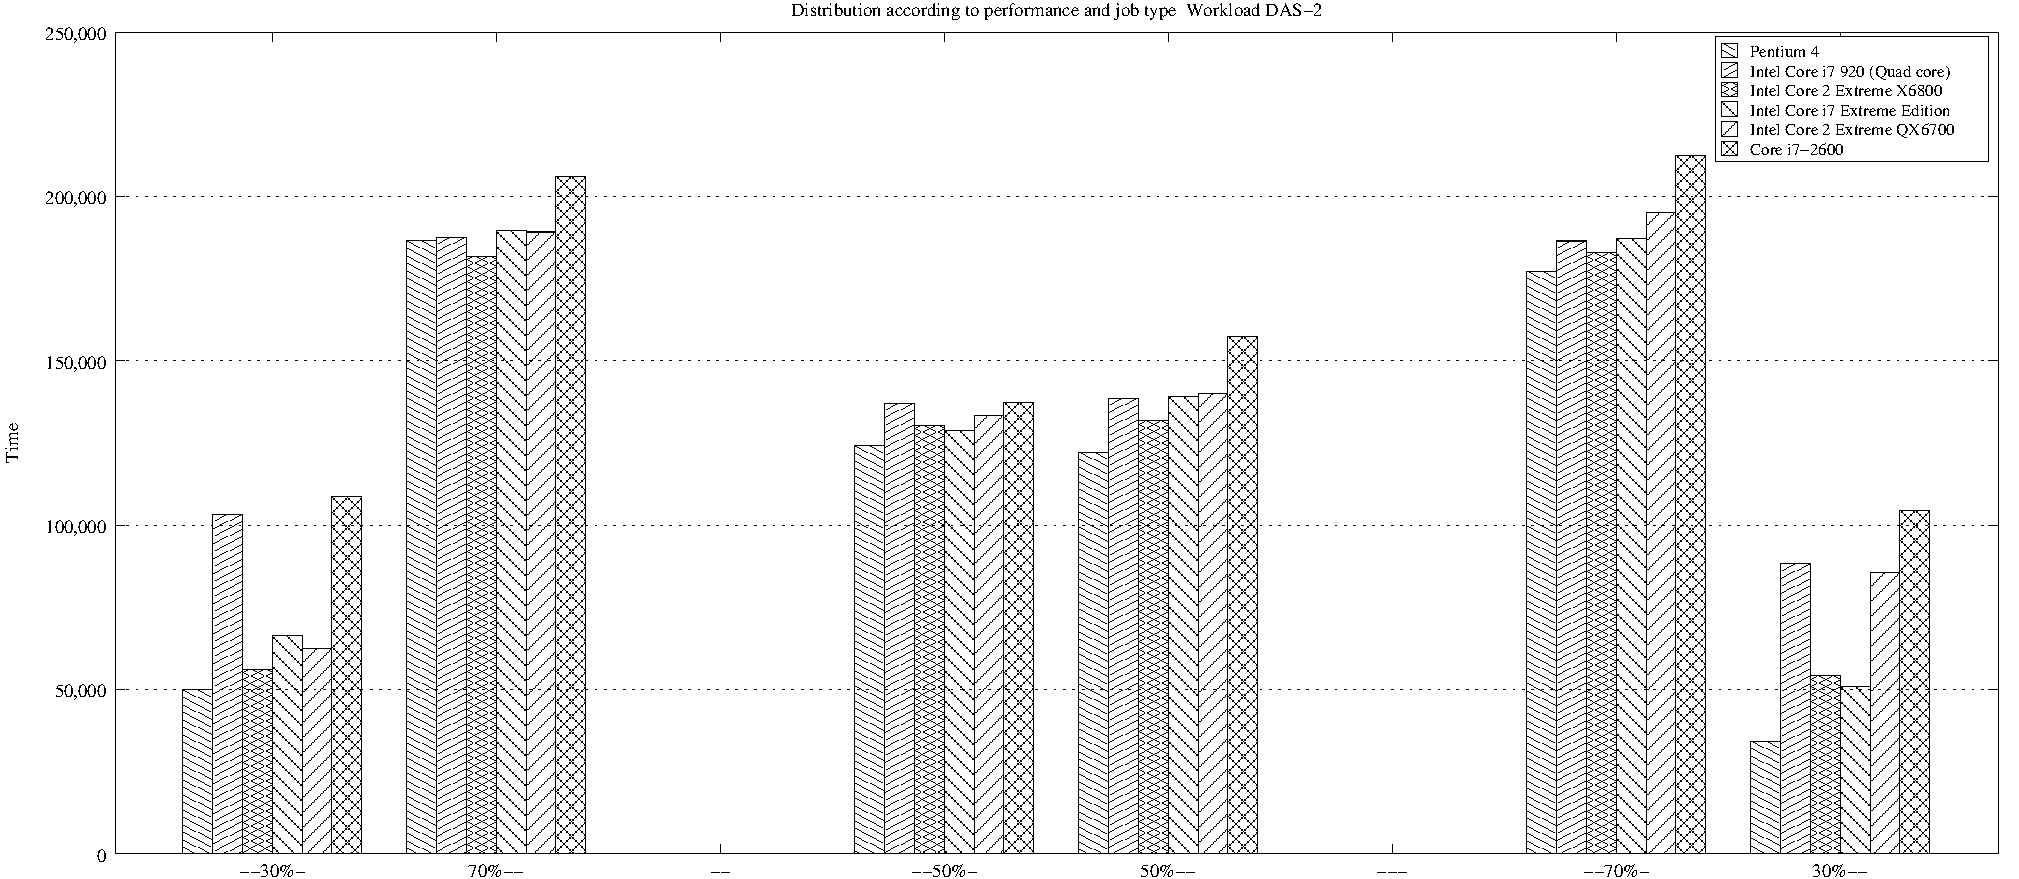
\includegraphics[width=1.0\columnwidth]{case3_DAS}
    \caption{Performance under Job type constraint, DAS-2 Workload}
\label{jobtype2}
\end{figure}

\subsection{Experiment: Introducing pricing model and precedence constraint}
\label{case4}
In this phase of experiment pricing parameter is incorporated in resource model. Experimented result shows how pricing model can change the utilization of resources. Workload 5 \&  6 have been used for this experiment having 50\% of job with predecessor dependencies referred in Table~\ref{datasets}. \\
Resources which are both low in performance and poor in energy efficiency is cheap in price, whereas high performance resource with less energy dissipation figure is preferred. Jobs having low job cost or high time limit can afford to run on these cheap resources whereas high priority jobs demanding high performance run on costly resources. Trade off among performance, time of execution and cost have allowed jobs to be scheduled on various resources uniformly. In table ~\ref{tab:sharccase4} \& ~\ref{tab:dascasse4}  it is observed that resources have adhered to the makespan and all have 98\%+ execution time. Utilization percentage shows actual uptime or running time of resources. This reveals that all resources have been utilized properly. Even resources like Pentium 4 have 95\% utilization on average.
\begin{framed}
{\small A question might arise in reader's mind ``Why resource utilization is not 100 percent?''. Jobs are having some precedence constraints; and a job scheduled on its compatible resource might take a little longer time to complete, forcing dependent jobs to wait on other idle resource. }
\end{framed}
In our experiment we have given equal weight to cost pricing, utilization of resources, time limit constraint and makespan. The grid administrator can configure the weight function to obtain required schedule strategy from first pareto front in search space like one given in figure ~\ref{pareto}.

\begin{table}[ht]
\caption{Resource Utilization after introduction of Job constraint and pricing model Workload 6 (SHARCNET)}
\scalebox{0.65}{
\begin{tabular}{|l|l|r|r|r|r|r|}
    \hline \hline
ID	&	Resource	&	Pricing model	&	Execution time	&	Makespan \%age	&	Actual utilized time	&	Utilization \%age	\\	\hline
1	&	Pentium 4	&	0.05	&	12048592.25	&	98.01	&	11813044.19	&	98.04	\\	\hline
2	&	Pentium 4	&	0.05	&	12163752.56	&	98.95	&	11300235.12	&	92.90	\\	\hline
3	&	Pentium 4	&	0.05	&	12164478.67	&	98.95	&	11686679.20	&	96.07	\\	\hline
4	&	Intel Core i7 920 (Quad core)	&	0.1	&	12046834.85	&	97.99	&	11272379.33	&	93.57	\\	\hline
5	&	Intel Core i7 920 (Quad core)	&	0.1	&	12047842.36	&	98.00	&	11749485.96	&	97.52	\\	\hline
6	&	Intel Core 2 Extreme X6800	&	0.09	&	12048727.00	&	98.01	&	11734951.47	&	97.39	\\	\hline
7	&	Intel Core 2 Extreme X6800	&	0.09	&	12160673.18	&	98.92	&	11776008.86	&	96.83	\\	\hline
8	&	Intel Core i7 Extreme Edition	&	0.15	&	12162928.27	&	98.94	&	11422999.16	&	93.91	\\	\hline
9	&	Intel Core i7 Extreme Edition	&	0.15	&	12160661.70	&	98.92	&	11777797.37	&	96.85	\\	\hline
10	&	Intel Core 2 Extreme QX6700	&	0.165	&	12160968.73	&	98.92	&	11864565.48	&	97.56	\\	\hline
11	&	Intel Core 2 Extreme QX6700	&	0.165	&	12156329.05	&	98.89	&	11976902.34	&	98.52	\\	\hline
12	&	Intel Core 2 Extreme QX6700	&	0.165	&	12160817.18	&	98.92	&	11727719.11	&	96.43	\\	\hline
13	&	Intel Core 2 Extreme QX6700	&	0.165	&	12160965.55	&	98.92	&	11931317.99	&	98.11	\\	\hline
14	&	Core i7-2600	&	0.18	&	12293364.46	&	100.00	&	11959913.00	&	97.28	\\	\hline
15	&	Core i7-2600	&	0.18	&	12161210.37	&	98.92	&	12059303.00	&	99.16	\\	\hline \hline
\end{tabular}
}
\label{tab:sharccase4}
\end{table}

\begin{table}[h]
\caption{Resource Utilization after introduction of Job constraint and pricing model Workload 5 (DAS-2)}
\centering
\scalebox{0.65}{
    \begin{tabular}{|l|l|r|r|r|r|r|}
    \hline \hline
ID	&	Resource	&	Pricing model	&	Execution time	&	Makespan \%age	&	Actual utilized time	&	Utilization \%age	\\	\hline
1	&	Pentium 4	&	0.05	&	307118.82	&	99.20	&	280545.30	&	91.34	\\	\hline
2	&	Pentium 4	&	0.05	&	301366.18	&	97.34	&	270360.92	&	89.71	\\	\hline
3	&	Pentium 4	&	0.05	&	300697.12	&	97.12	&	270477.22	&	89.95	\\	\hline
4	&	Intel Core i7 920 (Quad core)	&	0.1	&	307367.74	&	99.28	&	273357.18	&	88.93	\\	\hline
5	&	Intel Core i7 920 (Quad core)	&	0.1	&	307456.72	&	99.31	&	283748.63	&	92.28	\\	\hline
6	&	Intel Core 2 Extreme X6800	&	0.09	&	305703.06	&	98.74	&	269904.98	&	88.28	\\	\hline
7	&	Intel Core 2 Extreme X6800	&	0.09	&	305227.13	&	98.59	&	276089.83	&	90.45	\\	\hline
8	&	Intel Core i7 Extreme Edition	&	0.15	&	305428.16	&	98.65	&	288772.30	&	94.54	\\	\hline
9	&	Intel Core i7 Extreme Edition	&	0.15	&	303222.35	&	97.94	&	278433.59	&	91.82	\\	\hline
10	&	Intel Core 2 Extreme QX6700	&	0.165	&	309606.43	&	100.00	&	291890.84	&	94.27	\\	\hline
11	&	Intel Core 2 Extreme QX6700	&	0.165	&	309296.74	&	99.90	&	291225.75	&	94.15	\\	\hline
12	&	Intel Core 2 Extreme QX6700	&	0.165	&	305602.29	&	98.71	&	288181.42	&	94.29	\\	\hline
13	&	Intel Core 2 Extreme QX6700	&	0.165	&	303673.86	&	98.08	&	297436.40	&	97.94	\\	\hline
14	&	Core i7-2600	&	0.18	&	308464.86	&	99.63	&	303151.00	&	98.27	\\	\hline
15	&	Core i7-2600	&	0.18	&	308339.70	&	99.59	&	303203.00	&	98.33	\\	\hline \hline
\end{tabular}
}
\label{tab:dascasse4}
\end{table}
\subsection{Experiment with all constraints}
In this section we have incorporated all the constraints and evaluated our scheduler on workload 7 and 8 referred in Table~\ref{datasets}. Experiment is performed on 12 and 24 resources. For the sake of understanding equal number of resources for both type of jobs have been taken. \\
Results are given in Table ~\ref{case5das}, ~\ref{case5sha}, ~\ref{case5das24} and ~\ref{case5sha24}. There is no big difference with the result of Table~\ref{tab:dascasse4} and ~\ref{tab:sharccase4}. In this result, it is  observed that utilization percentage have dropped a little. Since jobs now have inter-resource type job dependencies utilization percentage drop is reasonable. Other performance parameter holds good. \\
An example of pareto front for this experiment is given in Figure~\ref{pareto3}  
\begin{figure}[h]
    \centering
    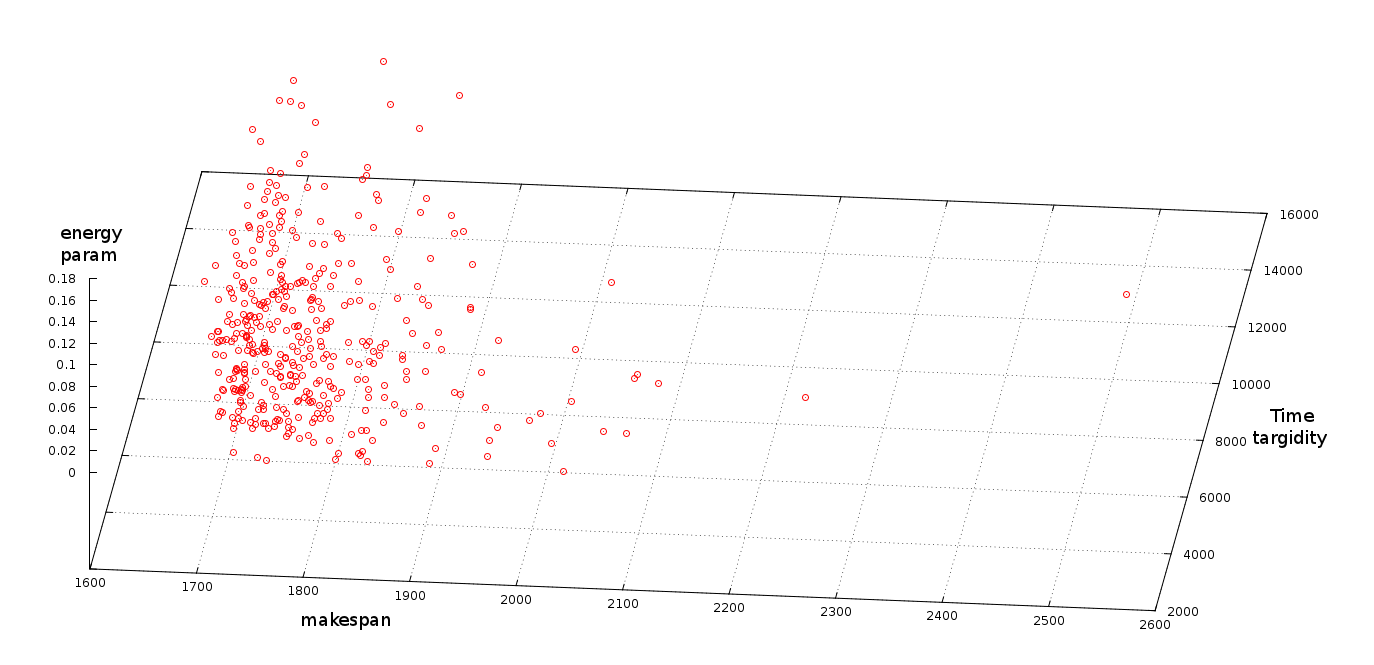
\includegraphics[width=1.0\columnwidth]{pareto3}
    \caption{Pareto front in experiment under all constraint}
    \label{pareto3}    
\end{figure}
    

\begin{table}[h]
\centering
\caption{Resource Utilization under all constraints on Workload DAS-2}
\scalebox{0.65}{
\begin{tabular}{|l|l|r|r|r|r|r|}
\hline \hline
ID	&	Resource	&	Pricing model	&	Execution time	&	Makespan \%age	&	Actual utilized time	&	Utilization \%age	\\	\hline
1	&	Pentium 4	&	0.05	&	388054.55346	&	95.31	&	337986.508894	&	87.10	\\	\hline
3	&	Intel Core i7 920 (Quad core)	&	0.1	&	390646.860537	&	95.95	&	362241.059321	&	92.72	\\	\hline
5	&	Intel Core 2 Extreme X6800	&	0.09	&	391917.860219	&	96.26	&	357671.610452	&	91.26	\\	\hline
7	&	Intel Core i7 Extreme Edition	&	0.15	&	389061.135613	&	95.56	&	367173.559685	&	94.37	\\	\hline
9	&	Intel Core 2 Extreme QX6700	&	0.165	&	389834.143125	&	95.75	&	368452.037427	&	94.51	\\	\hline
11	&	Core i7-2600	&	0.18	&	394967.616183	&	97.01	&	365376	&	92.50	\\	\hline
2	&	Pentium 4	&	0.05	&	407130.811479	&	100.00	&	362875.39219	&	89.12	\\	\hline
4	&	Intel Core i7 920 (Quad core)	&	0.1	&	406698.612175	&	99.89	&	343454.864029	&	84.44	\\	\hline
6	&	Intel Core 2 Extreme X6800	&	0.09	&	403146.303747	&	99.02	&	348012.012859	&	86.32	\\	\hline
8	&	Intel Core i7 Extreme Edition	&	0.15	&	402622.406754	&	98.89	&	378981.878416	&	94.12	\\	\hline
10	&	Intel Core 2 Extreme QX6700	&	0.165	&	405572.293961	&	99.62	&	385571.358202	&	95.06	\\	\hline
12	&	Core i7-2600	&	0.18	&	394268.616183	&	96.84	&	374894	&	95.08	\\	\hline \hline
\end{tabular}
}
\label{case5das}
\end{table}

\begin{table}[h]
\centering
\caption{Resource Utilization under all constraints on Workload SHARCNET }
\scalebox{0.65}{
    \begin{tabular}{|l|l|r|r|r|r|r|}
    \hline \hline
ID	&	Resource	&	Pricing model	&	Execution time	&	Makespan \%age	&	Actual utilized time	&	Utilization \%age	\\	\hline
1	&	Pentium 4	&	0.05	&	15856966.328786	&	99.65	&	14643863.906402	&	92.34	\\	\hline
3	&	Intel Core i7 920 (Quad core)	&	0.1	&	15777189.495383	&	99.14	&	14224208.443954	&	90.15	\\	\hline
5	&	Intel Core 2 Extreme X6800	&	0.09	&	15777954.142035	&	99.15	&	14347179.713218	&	90.93	\\	\hline
7	&	Intel Core i7 Extreme Edition	&	0.15	&	15853934.301256	&	99.63	&	14962167.332284	&	94.37	\\	\hline
9	&	Intel Core 2 Extreme QX6700	&	0.165	&	15855065.258749	&	99.63	&	14971170.083674	&	94.42	\\	\hline
11	&	Core i7-2600	&	0.18	&	15807884.835386	&	99.34	&	14039647	&	88.81	\\	\hline
2	&	Pentium 4	&	0.05	&	15855945.977623	&	99.64	&	15192585.514258	&	95.81	\\	\hline
4	&	Intel Core i7 920 (Quad core)	&	0.1	&	15856889.388767	&	99.65	&	15492772.72683	&	97.70	\\	\hline
6	&	Intel Core 2 Extreme X6800	&	0.09	&	15856577.788845	&	99.64	&	15509484.322644	&	97.81	\\	\hline
8	&	Intel Core i7 Extreme Edition	&	0.15	&	15808788.880171	&	99.34	&	15123906.518069	&	95.66	\\	\hline
10	&	Intel Core 2 Extreme QX6700	&	0.165	&	15913317.542563	&	100.00	&	15439774.23157	&	97.02	\\	\hline
12	&	Core i7-2600	&	0.18	&	15884947.971385	&	99.82	&	15685884	&	98.74	\\	\hline \hline
\end{tabular}
}
\label{case5sha}
\end{table}
\begin{table}[h]
\centering
\caption{Resource Utilization under all constraints on Workload SHARCNET }
\scalebox{0.65}{
    \begin{tabular}{|l|l|r|r|r|r|r|}
    \hline \hline
ID	&	Resource	&	Pricing model	&	Execution time	&	Makespan \%age	&	Actual utilized time	&	Utilization Percentage	\\	\hline
1	&	Pentium 4	&	0.05	&	8243698.72	&	99.49	&	7556234.165463	&	91.66	\\	\hline
2	&	Pentium 4	&	0.05	&	7275262.72	&	87.81	&	6253412.084217	&	85.95	\\	\hline
3	&	Intel Core i7 920 (Quad core)	&	0.1	&	7682671.48	&	92.72	&	6326204.11	&	82.34	\\	\hline
4	&	Intel Core i7 920 (Quad core)	&	0.1	&	8233315.82	&	99.37	&	7351339.16	&	89.28	\\	\hline
5	&	Intel Core 2 Extreme X6800	&	0.09	&	8117606.74	&	97.97	&	7269743.03	&	89.55	\\	\hline
6	&	Intel Core 2 Extreme X6800	&	0.09	&	8118002.88	&	97.98	&	7072373.18	&	87.11	\\	\hline
7	&	Intel Core i7 Extreme Edition	&	0.15	&	8117468.76	&	97.97	&	7183725.78	&	88.49	\\	\hline
8	&	Intel Core i7 Extreme Edition	&	0.15	&	8244584.64	&	99.50	&	7426916.89	&	90.08	\\	\hline
9	&	Intel Core 2 Extreme QX6700	&	0.165	&	8117904.66	&	97.98	&	7220275.87	&	88.94	\\	\hline
10	&	Intel Core 2 Extreme QX6700	&	0.165	&	8119335.22	&	97.99	&	7202661.19	&	88.70	\\	\hline
11	&	Core i7-2600	&	0.18	&	8229761.81	&	99.33	&	7763631	&	94.33	\\	\hline
12	&	Core i7-2600	&	0.18	&	8244728.91	&	99.51	&	7615311	&	92.36	\\	\hline
13	&	Pentium 4	&	0.05	&	8119374.38	&	97.99	&	7906705.979229	&	97.38	\\	\hline
14	&	Pentium 4	&	0.05	&	8231574.39	&	99.35	&	7705017.3826	&	93.60	\\	\hline
15	&	Intel Core i7 920 (Quad core)	&	0.1	&	8229150.06	&	99.32	&	7628743.04	&	92.70	\\	\hline
16	&	Intel Core i7 920 (Quad core)	&	0.1	&	8117134.83	&	97.97	&	7339766.91	&	90.42	\\	\hline
17	&	Intel Core 2 Extreme X6800	&	0.09	&	8244402.12	&	99.50	&	7126312.76	&	86.43	\\	\hline
18	&	Intel Core 2 Extreme X6800	&	0.09	&	8120187.28	&	98.00	&	7600934.79	&	93.60	\\	\hline
19	&	Intel Core i7 Extreme Edition	&	0.15	&	8285650.01	&	100.00	&	8151742.16	&	98.38	\\	\hline
20	&	Intel Core i7 Extreme Edition	&	0.15	&	8230477.53	&	99.33	&	7746832.68	&	94.12	\\	\hline
21	&	Intel Core 2 Extreme QX6700	&	0.165	&	8232608.55	&	99.36	&	7776374.29	&	94.45	\\	\hline
22	&	Intel Core 2 Extreme QX6700	&	0.165	&	8230191.41	&	99.33	&	7517359.04	&	91.33	\\	\hline
23	&	Core i7-2600	&	0.18	&	8244461.91	&	99.50	&	7950420	&	96.43	\\	\hline
24	&	Core i7-2600	&	0.18	&	8244329.91	&	99.50	&	7745014	&	93.94	\\	\hline
\end{tabular}
}
\label{case5sha24}
\end{table}

\begin{table}[!h]
\centering
\caption{Resource Utilization under all constraints on Workload DAS-2 }
\scalebox{0.65}{
    \begin{tabular}{|l|l|r|r|r|r|r|}
    \hline \hline
ID	&	Resource	&	Pricing model	&	Execution time	&	Makespan \%age	&	Actual utilized time	&	Utilization Percentage	\\	\hline
1	&	Pentium 4	&	0.05	&	219982.24	&	97.21	&	163440.56	&	74.29	\\	\hline
2	&	Pentium 4	&	0.05	&	219542.01	&	97.02	&	174237.89	&	79.36	\\	\hline
3	&	Intel Core i7 920 (Quad core)	&	0.1	&	219052.01	&	96.80	&	165654.30	&	75.62	\\	\hline
4	&	Intel Core i7 920 (Quad core)	&	0.1	&	216803.93	&	95.81	&	184625.00	&	85.15	\\	\hline
5	&	Intel Core 2 Extreme X6800	&	0.09	&	219223.62	&	96.88	&	182191.65	&	83.10	\\	\hline
6	&	Intel Core 2 Extreme X6800	&	0.09	&	219492.39	&	97.00	&	174748.10	&	79.61	\\	\hline
7	&	Intel Core i7 Extreme Edition	&	0.15	&	219025.20	&	96.79	&	181810.38	&	83.00	\\	\hline
8	&	Intel Core i7 Extreme Edition	&	0.15	&	220180.92	&	97.30	&	188177.47	&	85.46	\\	\hline
9	&	Intel Core 2 Extreme QX6700	&	0.165	&	224356.86	&	99.15	&	177056.99	&	78.91	\\	\hline
10	&	Intel Core 2 Extreme QX6700	&	0.165	&	195262.07	&	86.29	&	171776.61	&	87.97	\\	\hline
11	&	Core i7-2600	&	0.18	&	219419.10	&	96.97	&	190443	&	86.79	\\	\hline
12	&	Core i7-2600	&	0.18	&	218241.87	&	96.45	&	199849	&	91.57	\\	\hline
13	&	Pentium 4	&	0.05	&	218245.15	&	96.45	&	193682.53	&	88.74	\\	\hline
14	&	Pentium 4	&	0.05	&	221455.49	&	97.87	&	179685.28	&	81.13	\\	\hline
15	&	Intel Core i7 920 (Quad core)	&	0.1	&	220399.63	&	97.40	&	173087.60	&	78.53	\\	\hline
16	&	Intel Core i7 920 (Quad core)	&	0.1	&	223197.97	&	98.64	&	184545.05	&	82.68	\\	\hline
17	&	Intel Core 2 Extreme X6800	&	0.09	&	223858.93	&	98.93	&	187562.65	&	83.78	\\	\hline
18	&	Intel Core 2 Extreme X6800	&	0.09	&	221743.64	&	97.99	&	189665.95	&	85.53	\\	\hline
19	&	Intel Core i7 Extreme Edition	&	0.15	&	225453.79	&	99.63	&	164904.97	&	73.14	\\	\hline
20	&	Intel Core i7 Extreme Edition	&	0.15	&	226286.04	&	100.00	&	178501.31	&	78.88	\\	\hline
21	&	Intel Core 2 Extreme QX6700	&	0.165	&	224749.06	&	99.32	&	188318.89	&	83.79	\\	\hline
22	&	Intel Core 2 Extreme QX6700	&	0.165	&	225663.04	&	99.72	&	184520.37	&	81.76	\\	\hline
23	&	Core i7-2600	&	0.18	&	222377.53	&	98.27	&	196349	&	88.29	\\	\hline
24	&	Core i7-2600	&	0.18	&	223615.40	&	98.82	&	201232	&	89.99	\\	\hline
\end{tabular}
}
\label{case5das24}
\end{table}


\section{Conclusion}
The main motive of this work is to provide a flexible scheduler keeping multiple objectives into consideration. The scheduler module yields best scheduling strategies on various parameters in a pareto front. This is upto grid administrator and dynamic grid environment to choose a scheduling strategy of its choice. For experimentation purpose we have put equal weights on each objective for choosing best scheduling strategy. \\
Our results clearly shows that our scheduler produces optimized schedule on multi-objective optimization environment. The scheduler is scalable with resources and can process an infinite queue of jobs. The scheduler responded well with the change of constraints and behaviour of grid and job model. All resources have adhered to the makespan, and utilization rate is also high inspite of precedence constraint. It is difficult to display minimization of cost and time targidity parameter in graph or table. However a live demo of search space graph with schedules/chromosomes on successive iteration of genetic algorithm can verify its authenticity (Refer to User's Manual in Appendix~\ref{userman}). 
\\

        \chapter{Conclusion and Future Work}
We have addressed the grid job scheduling problem with additional dimension i.e. introduced precedence constraint with heterogeneous resources and types. Scheduling jobs while keeping multiple objectives in consideration is a challenging task on a dynamic grid environment. Beyond that, scheduling in grid being a real time operation, the scheduler should produce result within few seconds or minutes. This  makes scheduling more difficult. \\
Our resource manager simulates dynamic grid environment by adding and dropping resources.  We have formularized minimization functions, created avant-garde crossover, mutation and selection operator, merged with existing technology of pareto based optimization technique. The scheduler module outputs a set of best schedules on each run and offer grid administrator a better grip in choosing a schedule compatible according to the grid environment at that moment.
Job-grouping technique for fine-grained jobs keeping precedence constraint and resource constraint accelerates the yield of scheduler. \\
Our job scheduler have not considered some real world scenarios like transfer of jobs  or input files from one cluster to another before executing it. Resources leaving grid unexpectedly have a huge impact of resource utilization and QoS given to the jobs. If scheduler somehow obtain knowledge about the behavior of resources from grid logs, MTTF(Mean Time to Failure); it can schedule accordingly. Mining grid logs and find behaviour of the resources and jobs is important in real world scenarios.
        \appendix
        \chapter{Job Scheduler Module User's Manual}
\label{userman}
This chapter explains how to run and configure our scheduler and its other components related to it. 
\section{System Requirements}
\begin{itemize}
\item Intel processor / AMD processor 2.0 GHz or better, RAM: 4 GB, with 500 MB of free storage space.
\item Linux OS (Ubuntu 10.10 / Fedora 13 / Linux mint or better )
\item C++ library
\item SSH services on resources/computers with key based login.
\item MPICH2 library with hydra(mpiexec) \cite{mpich2}
\item GNUPLOT software
\end{itemize}

\section{Installation}
Before executing the scheduler following steps are needed to be done :
\begin{itemize}
\item Extract ``modjs.zip'' 
\subitem \$ tar -xvzf modjs.zip
\item Compile the source code
\subitem \$ make
\item Go to folder ``resource''
\subitem \$ cd resource
\subitem \$ gcc -c resource\_manager.c -o resource
\item Enter available resource information in ``initial\_resource.in'' in specified format.
\item Copy any job file from "data" folder and name it "job.in" for e.g.
\subitem \$ cp data/DAS-2/job\_no\_pred.in job.in
\item prepare hostfile.txt with ip address or domain name of all resources.
\end{itemize}

\section{Execution}
Command to run the job scheduler follows :
\begin{itemize}
 \item mpiexec  -disable-hostname-propagation -hostfile hostfile.txt ./modjsg $<$plot$>$ $<$NUM\_JOBS$>$ $<$POPULATION$>$ $<$GENERATION$>$ $<$RANDOM\_INTEGER$>$
\item $<$plot$>$  - 0 (run without GNUPLOT), 1 (without GNUPLOT)
\item $<$NUM\_JOBS$>$ - Number of jobs to be scheduled on each run of the job scheduler module. Range [100,1000] multiplier of 4.
\item $<$POPULATION$>$ - Chromosome population for genetic algorithm range, Range [200,1000]
 \item $<$GENERATION$>$ - Iteration in genetic algorithm, Range [50,300]
\item $<$RANDOM\_INTEGER$>$ - Any integer for randomize function seed.\\
e.g. \$ mpiexec  -disable-hostname-propagation -hostfile hostfile.txt ./modjsg 0 100 400 300 432421 \\
\item Command to run resource manager : 
\subitem \$ cd resource 
\subitem \$ ./resource 
\end{itemize}

To configure the selection criteria of schedule after final population of efficient schedule has been generated modify weight\_fun[] in report\_best() function in report.c file.

%	\input{Results2} 
	\backmatter
	\singlespacing
	\addcontentsline{toc}{chapter}{Bibliography}
%	\bibliographystyle{unsrt}
%       \bibliographystyle{alpha}
	\bibliographystyle{plain}
	\bibliography{references}
\end{document}